%  A simple AAU report template.
%  2015-05-08 v. 1.2.0
%  Copyright 2010-2015 by Jesper Kjær Nielsen <jkn@es.aau.dk>
%http://www.pedigreequery.com/generator/%
%  This is free software: you can redistribute it and/or modify
%  it under the terms of the GNU General Public License as published by
%  the Free Software Foundation, either version 3 of the License, or
%  (at your option) any later version.
%
%  This is distributed in the hope that it will be useful,
%  but WITHOUT ANY WARRANTY; without even the implied warranty of
%  MERCHANTABILITY or FITNESS FOR A PARTICULAR PURPOSE.  See the
%  GNU General Public License for more details.
%
%  You can find the GNU General Public License at <http://www.gnu.org/licenses/>.

% Variable for vores sprog navn
\newcommand\lang{PEAK+ }

\documentclass[12pt,twoside,a4paper,openright]{report}
%%%%%%%%%%%%%%%%%%%%%%%%%%%%%%%%%%%%%%%%%%%%%%%%
% Language, Encoding and Fonts
% http://en.wikibooks.org/wiki/LaTeX/Internationalization
%%%%%%%%%%%%%%%%%%%%%%%%%%%%%%%%%%%%%%%%%%%%%%%%
% Select encoding of your inputs. Depends on
% your operating system and its default input
% encoding. Typically, you should use
%   Linux  : utf8 (most modern Linux distributions)
%            latin1 
%   Windows: ansinew
%            latin1 (works in most cases)
%   Mac    : applemac
% Notice that you can manually change the input
% encoding of your files by selecting "save as"
% an select the desired input encoding. 
\usepackage[utf8]{inputenc}
% Make latex understand and use the typographic
%Font package
\usepackage{bbm}
% rules of the language used in the document.
\usepackage[danish,english]{babel}
% Use the palatino font
\usepackage[sc]{mathpazo}
\linespread{1.1}         % Palatino needs more leading (space between lines)
% Choose the font encoding
\usepackage[T1]{fontenc}
\usepackage{float}
%%%%%%%%%%%%%%%%%%%%%%%%%%%%%%%%%%%%%%%%%%%%%%%%
% Graphics and Tables
% http://en.wikibooks.org/wiki/LaTeX/Importing_Graphics
% http://en.wikibooks.org/wiki/LaTeX/Tables
% http://en.wikibooks.org/wiki/LaTeX/Colors
%%%%%%%%%%%%%%%%%%%%%%%%%%%%%%%%%%%%%%%%%%%%%%%%
% load a colour package
%table packages
\usepackage{graphicx}
\usepackage[table,xcdraw]{xcolor}

%Spacing package for math mode
\usepackage{amsmath}

%Additional math symbol package
\usepackage{turnstile}

\usepackage{xcolor}
\definecolor{aaublue}{RGB}{33,26,82}% dark blue
% The standard graphics inclusion package
\usepackage{graphicx}
% package for turning pages into landscape mode
\usepackage{lscape}
% Set up how figure and table captions are displayed
\usepackage{caption}
% Allows for multiple rows in tables
\usepackage{multirow}

\captionsetup{%
  font=footnotesize,% set font size to footnotesize
  labelfont=bf % bold label (e.g., Figure 3.2) font
}
% Make the standard latex tables look so much better
\usepackage{array,booktabs}
% Enable the use of frames around, e.g., theorems
% The framed package is used in the example environment
\usepackage{framed}
\definecolor{editorGray}{rgb}{0.95, 0.95, 0.95}
\definecolor{editorOcher}{rgb}{1, 0.5, 0} % #FF7F00 -> rgb(239, 169, 0)
\definecolor{editorGreen}{rgb}{0, 0.5, 0} % #007C00 -> rgb(0, 124, 0)
\definecolor{mGreen}{rgb}{0,0.6,0}
\definecolor{mGray}{rgb}{0.5,0.5,0.5}
\definecolor{mPurple}{rgb}{0.58,0,0.82}
\definecolor{backgroundColour}{rgb}{0.95,0.95,0.92}

\usepackage{upquote}
\usepackage{listings}

\lstdefinelanguage{scriptkid}{
 %morecomment = [l]{//},
 %morekeywords = {number, text, boolean, true, false, if, repeat, else, return, function},
 morekeywords={true, false, function, return, null, if,  while, do, else},
 ndkeywords={number, text, boolean, decimal},
  morecomment=[l]comment:,
  morestring=[b]",
  morestring=[b]',
  captionpos=b,
}

\lstdefinestyle{CStyle}{
    backgroundcolor=\color{backgroundColour},   
    commentstyle=\color{mGreen},
    keywordstyle=\color{magenta},
    numberstyle=\tiny\color{mGray},
    stringstyle=\color{mPurple},
    basicstyle=\footnotesize,
    breakatwhitespace=false,         
    breaklines=true,                 
    captionpos=b,                    
    keepspaces=true,                 
    numbers=left,                    
    numbersep=5pt,                  
    showspaces=false,                
    showstringspaces=false,
    showtabs=false,                  
    tabsize=2
}

\lstdefinelanguage{JavaScript}{
  morekeywords={true, false, function, return, null, if, is, while, do, else},
  morecomment=[s]{/*}{*/},
  morecomment=[l]//,
  morestring=[b]",
  morestring=[b]'
  captionpos=b,
}

\lstdefinelanguage{csharp}
{
 morecomment = [l]{//}, 
 morecomment = [l]{///},
 morecomment = [s]{/*}{*/},
 captionpos=b,
 morestring=[b]", 
 sensitive = true,
 morekeywords = {abstract,  event,  new,  struct,
   as,  explicit,  null,  switch,
   base,  extern,  object,  this,
   bool,  false,  operator,  throw,
   break,  finally,  out,  true,
   byte,  fixed,  override,  try,
   case,  float,  params,  typeof,
   catch,  for,  private,  uint,
   char,  foreach,  protected,  ulong,
   checked,  goto,  public,  unchecked,
   class,  if,  readonly,  unsafe,
   const,  implicit,  ref,  ushort,
   continue,  in,  return,  using,
   decimal,  int,  sbyte,  virtual,
   default,  interface,  sealed,  volatile,
   delegate,  internal,  short,  void,
   do,  is,  sizeof,  while,
   double,  lock,  stackalloc,   
   else,  long,  static,   
   enum,  namespace,  string}
}

\lstdefinelanguage{HTML5}{
        language=html,
        sensitive=true, 
        alsoletter={<>=-},
        otherkeywords={
        % HTML tags
        <html>, <head>, <title>, </title>, <meta, />, </head>, <body>,
        <canvas, \/canvas>, <script>, </script>, </body>, </html>, <!, html>, <style>, </style>, ><
        },  
        ndkeywords={
        % General
        =,
        % HTML attributes
        charset=, id=, width=, height=,
        % CSS properties
        border:, transform:, -moz-transform:, transition-duration:, transition-property:, transition-timing-function:
        },  
        morecomment=[s]{<!--}{-->},
        tag=[s]
}

\lstdefinelanguage{CSS}{
  otherkeywords={background, max, animation, flex-direction, gap, text-align, overflow, opacity, color,background-image:,margin,padding,font,weight,display,position,top,left,right,bottom,list,style,border,size,space,min,width, transition:, transform:, transition-property, transition-duration, transition-timing-function},	
  sensitive=true,
  morecomment=[l]{//},
  morecomment=[s]{/*}{*/},
  alsoletter={:},
  alsodigit={-},
  ndkeywords={auto, rem, fade, ms, ease-in-out, forwards, px, flex, column, center, #, hidden, none, translateX, both, solid, relative, scale, white}
}

\lstset{%
    % Basic design
    backgroundcolor=\color{editorGray},
    basicstyle={\small\ttfamily},   
    frame=l,
    % Line numbers
    xleftmargin={0.75cm},
    numbers=left,
    stepnumber=1,
    firstnumber=1,
    numberfirstline=true,
    % Code design   
    keywordstyle=\color{blue}\bfseries,
    commentstyle=\color{editorGreen}\ttfamily,
    ndkeywordstyle=\color{cyan}\bfseries,
    stringstyle=\color{editorOcher},
    % Code
    alsodigit={.:;},
    tabsize=4,
    showtabs=false,
    showspaces=false,
    showstringspaces=false,
    extendedchars=true,
    breaklines=true,        
    % Support for German umlauts
    literate=%
    {Ö}{{\"O}}1
    {Ä}{{\"A}}1
    {Ü}{{\"U}}1
    {ß}{{\ss}}1
    {ü}{{\"u}}1
    {ä}{{\"a}}1
    {ö}{{\"o}}1
}

\usepackage{wrapfig}
\usepackage{lscape}
\usepackage{longtable}
\usepackage{comment}
%%%%%%%%%%%%%%%%%%%%%%%%%%%%%%%%%%%%%%%%%%%%%%%%
% Mathematics
% http://en.wikibooks.org/wiki/LaTeX/Mathematics
%%%%%%%%%%%%%%%%%%%%%%%%%%%%%%%%%%%%%%%%%%%%%%%%
% Defines new environments such as equation,
% align and split 
\usepackage{amsmath}
% Adds new math symbols
\usepackage{amssymb}
% Use theorems in your document
% The ntheorem package is also used for the example environment
% When using thmmarks, amsmath must be an option as well. Otherwise \eqref doesn't work anymore.
\usepackage[framed,amsmath,thmmarks]{ntheorem}

%%%%%%%%%%%%%%%%%%%%%%%%%%%%%%%%%%%%%%%%%%%%%%%%
% Page Layout
% http://en.wikibooks.org/wiki/LaTeX/Page_Layout
%%%%%%%%%%%%%%%%%%%%%%%%%%%%%%%%%%%%%%%%%%%%%%%%
% Change margins, papersize, etc of the document
\usepackage[
  inner=25mm,% left margin on an odd page
  outer=25mm,% right margin on an odd page
  bottom = 2.75cm,
  ]{geometry}
% Modify how \chapter, \section, etc. look
% The titlesec package is very configureable
\usepackage{titlesec}
\titleformat{\chapter}[display]{\normalfont\huge\bfseries}{\chaptertitlename\ \thechapter}{20pt}{\Huge}
\titleformat*{\section}{\normalfont\Large\bfseries}
\titleformat*{\subsection}{\normalfont\large\bfseries}
\titleformat*{\subsubsection}{\normalfont\normalsize\bfseries}
%\titleformat*{\paragraph}{\normalfont\normalsize\bfseries}
%\titleformat*{\subparagraph}{\normalfont\normalsize\bfseries}

% Clear empty pages between chapters
\let\origdoublepage\cleardoublepage
\newcommand{\clearemptydoublepage}{%
  \clearpage
  {\pagestyle{empty}\origdoublepage}%
}
\let\cleardoublepage\clearemptydoublepage

% Change the headers and footers
\usepackage{fancyhdr}
\pagestyle{fancy}
\fancyhf{} %delete everything
\renewcommand{\headrulewidth}{0pt} %remove the horizontal line in the header
\fancyhead[RE]{\small\nouppercase\leftmark} %even page - chapter title
\fancyhead[LO]{\small\nouppercase\rightmark} %uneven page - section title
\fancyhead[LE,RO]{\thepage} %page number on all pages
% Do not stretch the content of a page. Instead,
% insert white space at the bottom of the page
\raggedbottom
% Enable arithmetics with length. Useful when
% typesetting the layout.
\usepackage{calc}

%%%%%%%%%%%%%%%%%%%%%%%%%%%%%%%%%%%%%%%%%%%%%%%%
% Bibliography
% http://en.wikibooks.org/wiki/LaTeX/Bibliography_Management
%%%%%%%%%%%%%%%%%%%%%%%%%%%%%%%%%%%%%%%%%%%%%%%%
\usepackage[backend=bibtex,
  bibencoding=utf8
  ]{biblatex}
\addbibresource{bib/mybib}

%%%%%%%%%%%%%%%%%%%%%%%%%%%%%%%%%%%%%%%%%%%%%%%%
% Misc
%%%%%%%%%%%%%%%%%%%%%%%%%%%%%%%%%%%%%%%%%%%%%%%%
% Add bibliography and index to the table of
% contents
\usepackage[nottoc]{tocbibind}
% Add the command \pageref{LastPage} which refers to the
% page number of the last page
\usepackage{lastpage}
% Add todo notes in the margin of the document
\usepackage[
%  disable, %turn off todonotes
  colorinlistoftodos, %enable a coloured square in the list of todos
  textwidth=\marginparwidth, %set the width of the todonotes
  textsize=scriptsize, %size of the text in the todonotes
  ]{todonotes}

%%%%%%%%%%%%%%%%%%%%%%%%%%%%%%%%%%%%%%%%%%%%%%%%
% Hyperlinks
% http://en.wikibooks.org/wiki/LaTeX/Hyperlinks
%%%%%%%%%%%%%%%%%%%%%%%%%%%%%%%%%%%%%%%%%%%%%%%%
% Enable hyperlinks and insert info into the pdf
% file. Hypperref should be loaded as one of the 
% last packages
\usepackage{hyperref}
\hypersetup{%
	pdfpagelabels=true,%
	plainpages=false,%
	pdfauthor={Author(s)},%
	pdftitle={Title},%
	pdfsubject={Subject},%
	bookmarksnumbered=true,%
	colorlinks=false,%
	citecolor=black,%
	filecolor=black,%
	linkcolor=black,% you should probably change this to black before printing
	urlcolor=black,%
	pdfstartview=FitH%
}

\usepackage{color}
\definecolor{red}{rgb}{0.6,0,0} 
\definecolor{blue}{rgb}{0,0,0.6}
\definecolor{green}{rgb}{0,0.8,0}
\definecolor{cyan}{rgb}{0.0,0.6,0.6}


\newcommand{\newCommandName}{text to insert}% package inclusion and set up of the document
% see, e.g., http://en.wikibooks.org/wiki/LaTeX/Formatting#Hyphenation
% for more information on word hyphenation
\hyphenation{ex-am-ple hy-phen-a-tion short}
\hyphenation{long la-tex}% 
%  A simple AAU report template.
%  2015-05-08 v. 1.2.0
%  Copyright 2010-2015 by Jesper Kjær Nielsen <jkn@es.aau.dk>
%
%  This is free software: you can redistribute it and/or modify
%  it under the terms of the GNU General Public License as published by
%  the Free Software Foundation, either version 3 of the License, or
%  (at your option) any later version.
%
%  This is distributed in the hope that it will be useful,
%  but WITHOUT ANY WARRANTY; without even the implied warranty of
%  MERCHANTABILITY or FITNESS FOR A PARTICULAR PURPOSE.  See the
%  GNU General Public License for more details.
%
%  You can find the GNU General Public License at <http://www.gnu.org/licenses/>.
%
%
%
% see, e.g., http://en.wikibooks.org/wiki/LaTeX/Customizing_LaTeX#New_commands
% for more information on how to create macros

%%%%%%%%%%%%%%%%%%%%%%%%%%%%%%%%%%%%%%%%%%%%%%%%
% Macros for the titlepage
%%%%%%%%%%%%%%%%%%%%%%%%%%%%%%%%%%%%%%%%%%%%%%%%
%Creates the aau titlepage
\newcommand{\aautitlepage}[3]{%
  {
    %set up various length
    \ifx\titlepageleftcolumnwidth\undefined
      \newlength{\titlepageleftcolumnwidth}
      \newlength{\titlepagerightcolumnwidth}
    \fi
    \setlength{\titlepageleftcolumnwidth}{0.5\textwidth-\tabcolsep}
    \setlength{\titlepagerightcolumnwidth}{\textwidth-2\tabcolsep-\titlepageleftcolumnwidth}
    %create title page
    \thispagestyle{empty}
    \noindent%
    \begin{tabular}{@{}ll@{}}
      \parbox{\titlepageleftcolumnwidth}{
        \iflanguage{danish}{%
          \includegraphics[width=\titlepageleftcolumnwidth]{Files/figures/aau_logo_da}
        }{%
          \includegraphics[width=0.4\textwidth]{Files/figures/aau_logo_en}
        }
      } &
      \parbox{\titlepagerightcolumnwidth}{\raggedleft\sf\small
        #2
      }\bigskip\\
       #1 &
      \parbox[t]{\titlepagerightcolumnwidth}{%
      \textbf{Abstract:}\bigskip\par
        \fbox{\parbox{\titlepagerightcolumnwidth-2\fboxsep-2\fboxrule}{%
          #3
        }}
      }\\
    \end{tabular}
    \vfill
    \iflanguage{danish}{%
      \noindent{\footnotesize\emph{Rapportens indhold er frit tilgængeligt, men offentliggørelse (med kildeangivelse) må kun ske efter aftale med forfatterne.}}
    }{%
      \noindent{\footnotesize\emph{The content of this report is freely available, but publication (with reference) may only be pursued due to agreement with the author.}}
    }
    \clearpage
  }
}

%Create english project info
\newcommand{\englishprojectinfo}[8]{%
  \parbox[t]{\titlepageleftcolumnwidth}{
    \textbf{Title:}\\ #1\bigskip\par
    \textbf{Theme:}\\ #2\bigskip\par
    \textbf{Project Period:}\\ #3\bigskip\par
    \textbf{Project Group:}\\ #4\bigskip\par
    \textbf{Participant(s):}\\ #5\bigskip\par
    \textbf{Supervisor(s):}\\ #6\bigskip\par
    \textbf{Copies:} #7\bigskip\par
    \textbf{Page Numbers:} \pageref{LastPage}\bigskip\par
    \textbf{Date of Completion:}\\ #8
  }
}

%Create danish project info
\newcommand{\danishprojectinfo}[8]{%
  \parbox[t]{\titlepageleftcolumnwidth}{
    \textbf{Titel:}\\ #1\bigskip\par
    \textbf{Tema:}\\ #2\bigskip\par
    \textbf{Projektperiode:}\\ #3\bigskip\par
    \textbf{Projektgruppe:}\\ #4\bigskip\par
    \textbf{Deltager(e):}\\ #5\bigskip\par
    \textbf{Vejleder(e):}\\ #6\bigskip\par
    \textbf{Oplagstal:} #7\bigskip\par
    \textbf{Sidetal:} \pageref{LastPage}\bigskip\par
    \textbf{Afleveringsdato:}\\ #8
  }
}


%%%%%%%%%%%%%%%%%%%%%%%%%%%%%%%%%%%%%%%%%%%%%%%%
% An example environment
%%%%%%%%%%%%%%%%%%%%%%%%%%%%%%%%%%%%%%%%%%%%%%%%
\theoremheaderfont{\normalfont\bfseries}
\theorembodyfont{\normalfont}
\theoremstyle{break}
\def\theoremframecommand{{\color{gray!50}\vrule width 5pt \hspace{5pt}}}
\newshadedtheorem{exa}{Example}[chapter]
\newenvironment{example}[1]{%
		\begin{exa}[#1]
}{%
		\end{exa}
}% my new macros
\usepackage{enumitem}

\begin{document}
%frontmatter
\pagestyle{empty} %disable headers and footers
\pagenumbering{roman} %use roman page numbering in the frontmatter
%  A simple AAU report template.
%  2015-05-08 v. 1.2.0
%  Copyright 2010-2015 by Jesper Kjær Nielsen <jkn@es.aau.dk>
%
%  This is free software: you can redistribute it and/or modify
%  it under the terms of the GNU General Public License as published by
%  the Free Software Foundation, either version 3 of the License, or
%  (at your option) any later version.
%
%  This is distributed in the hope that it will be useful,
%  but WITHOUT ANY WARRANTY; without even the implied warranty of
%  MERCHANTABILITY or FITNESS FOR A PARTICULAR PURPOSE.  See the
%  GNU General Public License for more details.
%
%  You can find the GNU General Public License at <http://www.gnu.org/licenses/>.
%
\pdfbookmark[0]{Front page}{label:frontpage}%
\begin{titlepage}
  \addtolength{\hoffset}{0.5\evensidemargin-0.5\oddsidemargin} %set equal margins on the frontpage - remove this line if you want default margins
  \noindent%
  \begin{tabular}{@{}p{\textwidth}@{}}
    \toprule[2pt]
    \midrule
    \vspace{0.2cm}
    \begin{center}
    \Huge{\textbf{
    \lang \\
    (Programming Education And Knowledge+) % insert your title here
    }}
    \end{center}
    \begin{center}
      \Large{
        - P4 -% insert your subtitle here
      }
    \end{center}
    \vspace{0.2cm}\\
    \midrule
    \toprule[2pt]
  \end{tabular}
  \vspace{3 cm}
\begin{figure}[H]

\includegraphics[width=0.35\textwidth]{Files/logo.png}
\centering
\end{figure}
  \begin{center}
    {\large
      Project Report%Insert document type (e.g., Project Report)
    }\\
    \vspace{0.2cm}
    {\Large
      SW4-01%Insert your group name or real names here
    }
  \end{center}
  \vfill
  \begin{center}
  Aalborg University\\
  Department of Computer Science
  \end{center}
\end{titlepage}
\clearpage
\thispagestyle{empty}
{\small
\strut\vfill % push the content to the bottom of the page
\noindent Copyright \copyright{} Aalborg University 2023\par
\vspace{0.2cm}
\noindent Overleaf, Discord, Jira, Outlook.com, GitHub, Microsoft Teams, ChatGPT, Tablesgenerator.
}
\clearpage
\pdfbookmark[0]{English title page}{label:titlepage_en}
\aautitlepage{%
  \englishprojectinfo{
     PEAK+ - Programming Education and Knowledge+%title
  }{%
     Design, definition and implementation of programming languages %theme
  }{%
    Spring Semester 2023 %project period
  }{%
    SW4-01 % project group
  }{%
    %list of group members
    Charlotte Sundahl Elleby\\ 
    Christian Povlsen\\
    Nichlas Seerup Hjorth\\
    Rasmus Bartholomay Vikøren Borup\\
    Thomas Bjeldbak Madsen\\
    Thomas Ilum Andersen
  }{%
    %list of supervisors
    Lone Leth Thomsen 
  }{%
    1 % number of printed copies
  }{%
    \today % date of completion
  }%
}{%department and address
  \textbf{Department of Computer Science}\\
  Aalborg University\\
  \href{http://www.aau.dk}{http://www.aau.dk}
}{% the abstract
The learning curve of a new programming language for beginners who have experience with block-based languages is equally difficult for beginners, with the same amount of experience, but with text-based languages. This provides a need for a language that introduces beginners to the textual industry-standard programming languages. This report details the development and creation of \lang, a programming language that aims to fulfil this aforementioned need. The necessary syntax for \lang was developed through an analysis of existing programming languages, including Scratch, Quorum, C, and Python. The languages were analyzed with Sebesta's language criteria. Through this analysis, the syntax and semantics of \lang were designed. A functional compiler was built, by going through 3 essential phases: syntax analysis, contextual analysis, and code generation. ANTLR was used as a parser generator tool, and a visitor pattern, developed in C\# was used to traverse the compiler. The compiler was tested through unit, integration, and acceptance testing. The language was concluded to have theoretically solved the need for a language between block-based and text-based programming languages, however, to fully conclude a successful solution, proper user testing must be completed. 
}

\begin{comment}
\cleardoublepage
{\selectlanguage{danish}
\pdfbookmark[0]{Danish title page}{label:titlepage_da}
\aautitlepage{%
  \danishprojectinfo{
    Rapportens titel %title
  }{%
    Semestertema %theme
  }{%
    Efterårssemestret 2010 %project period
  }{%
    XXX % project group
  }{%
    %list of group members
    Forfatter 1\\ 
    Forfatter 2\\
    Forfatter 3
  }{%
    %list of supervisors
    Vejleder 1\\
    Vejleder 2
  }{%
    1 % number of printed copies
  }{%
    \today % date of completion
  }%
}{%department and address
  \textbf{Elektronik og IT}\\
  Aalborg Universitet\\
  \href{http://www.aau.dk}{http://www.aau.dk}
}{% the abstract
  Her er resuméet
}}
\end{comment}
\cleardoublepage
\pdfbookmark[0]{Contents}{label:contents}
\pagestyle{fancy} %enable headers and footers again
\chapter*{Preface\markboth{Preface}{Preface}}\label{ch:preface}
\addcontentsline{toc}{chapter}{Preface}

This report was written by CS-23-SW4-01, a group of students in the fourth semester of studying Software at Aalborg University. 

\subsubsection{Code snippets}
The report contains code snippets. In some snippets, parts of the code that are less relevant to the points being made have been omitted. This is indicated with [. . .] as seen in listing \ref{list:CodeSnippetExample}.

\begin{lstlisting}[language = csharp, firstnumber=1, label={list:CodeSnippetExample},caption=Example of the structure of a code snippet. Lines 2-4 indicate omitted code]
//First part of code snippet
.
.
.
//Continuation of the code snippet
\end{lstlisting}

\subsubsection{Target audience}
The target audience for this project is computer science students at the beginning of their fourth semester. The target group for the product is high school students who are learning programming for the first time. 

\subsubsection{Application of theory}
The report is structured in a way so that the necessary theory for a section or subsection is presented to the reader at the start of the section. Subsequently, the theory will be applied in a way that assumes the reader understands it.   

\subsubsection{Acknowledgements}
We would like to express our gratitude to our supervisor Lone Leth Thomsen for her guidance and support throughout the project. Furthermore, we would like to thank Morten Konggaard Schou for assisting us with the semantic definitions for \lang.  


\newpage

\vspace{\baselineskip}\hfill Aalborg University, \today
\vfill\noindent
\begin{minipage}[b]{0.45\textwidth}
 \centering
 \rule{\textwidth}{0.5pt}\\
  Charlotte Sundahl Elleby\\
 {\footnotesize <celleb21@student.aau.dk>}
\end{minipage}
\hfill
\begin{minipage}[b]{0.45\textwidth}
 \centering
 \rule{\textwidth}{0.5pt}\\
  Christian Povlsen\\
 {\footnotesize <cpovls21@student.aau.dk>}
\end{minipage}
\vspace{3\baselineskip}
\hfill
\vfill\noindent
\begin{minipage}[b]{0.45\textwidth}
 \centering
 \rule{\textwidth}{0.5pt}\\
  Nichlas Seerup Hjorth\\
 {\footnotesize <nhjor21@student.aau.dk>}
\end{minipage}
\hfill
\begin{minipage}[b]{0.45\textwidth}
 \centering
 \rule{\textwidth}{0.5pt}\\
  Rasmus Bartholomay Vikøren Borup\\
 {\footnotesize <rborup21@student.aau.dk>}
\end{minipage}
\vspace{3\baselineskip}
\hfill
\vfill\noindent
\begin{minipage}[b]{0.45\textwidth}
 \centering
 \rule{\textwidth}{0.5pt}\\
  Thomas Bjeldbak Madsen\\
 {\footnotesize <tbma21@student.aau.dk>}
\end{minipage}
\hfill
\begin{minipage}[b]{0.45\textwidth}
 \centering
 \rule{\textwidth}{0.5pt}\\
  Thomas Ilum Andersen\\
 {\footnotesize <tian21@student.aau.dk>}
\end{minipage}
\vspace{3\baselineskip}
\hfill



\tableofcontents
\cleardoublepage
%mainmatter
\pagenumbering{arabic} %use arabic page numbering in the mainmatter
\chapter{Introduction}\label{ch:introduction}
In today's world, programming has become an important skill \cite{ProgrammingImportant}. However, for beginner programmers, the process of getting started with programming can be daunting due to the steep learning curve. Existing programming languages can be complex, requiring significant prior knowledge, and making it challenging for beginner programmers to pursue programming as a career or hobby \cite{LearningCodeIsHard}.\\
This problem produces an increasing demand for the creation of new programming languages that are specifically designed for beginners\cite{demandforlanguages}. These languages should be user-friendly, easy to learn, and provide an immersive experience that encourages learners to hone their skills.\\

\noindent As an introduction to programming, block-based languages are very commonly used \cite{FromBlockToText}, but as these languages are limited to the block structure, the beginner programmer at some point has to switch to a text-based language. Even though learning block-based languages develops computational thinking \cite{FromBlockToText}, transitioning to text-based programming is difficult. It requires persistence to remember the syntax and semantics of the language and programming courses tend to have a high failure rate
\cite{FactorsDifficultiesInProgramming}.\\

\noindent The aim of this report is to document the development of a new programming language \lang, targeted towards beginner programmers in high school. This includes examining the rationale behind developing a new programming language for beginners and the essential features of such a language.
The specification needed for a beginner-friendly programming language will be discovered by analyzing and comparing four programming languages: Scratch, C, Python, and Quorum.

\noindent This report takes the reader through the different phases of creating a compiler for this new language: \lang.
\chapter{Problem analysis}\label{ch:ch2label}
%In today's world, programming has become an important skill \cite{ProgrammingImportant}. However, for beginners, the process of getting started with programming can be daunting due to the steep learning curve. Existing programming languages can be complex, requiring significant prior knowledge, and making it challenging for new learners to pursue programming as a career or hobby \cite{LearningCodeIsHard}.

%This problem produces an increasing demand for the creation of new programming languages that are specifically designed for beginners\cite{demandforlanguages}. These languages should be user-friendly, easy to learn, and provide an immersive experience that encourages learners to hone their skills. 

This chapter will analyze the difficulty of learning programming as a beginner programmer. It will cover some basic analysis of different programming languages with the aim of eventually comparing them, from the perspective of beginner programmers, to finally arrive at a concrete problem statement. The chapter will include facts from studies but also our own experience as beginner programmers.

\section{Learning programming }
As programming is an important skill worldwide \cite{ProgrammingImportant}, it is widely incorporated into the study curriculum of high schools and colleges. Learning text-based programming requires the student to learn, understand and remember the syntax and semantics of the language. Furthermore, the students have to evolve their computational thinking in order to solve programming problems. To learn these skills students have to be persistent in the effort of studying programming, and programming courses tend to have a high failure rate \cite{FactorsDifficultiesInProgramming}. Comparing these facts with our own experiences when being new programmers, it matches quite well. The learning curve required persistent activity and focus on the new content. \\

As an introduction to programming, block-based programming is an option. Block-based programming is mainly used to introduce children to programming, but it is also widely used in high school curricula \cite{FromBlockToText}.\\
Instead of writing lines of code and having to remember all the syntax, block-based programming is based on drag-and-drop blocks. Each block represents some function or action that the program should handle. This visual approach provides the user with an intuitive and accessible way to learn to program. The user can easily understand what they are doing and how to continue developing. Furthermore, it is quick to get easy tasks done and the user gets a visual response on what they have created \cite{FunTechBlockBased}.\\

Block-based programming has a positive impact on the motivation to learn programming and studies show that it evolves the student's computational thinking and learning of algorithmic skills \cite{FromBlockToText}. However, to continue developing as a developer, the student will reach a point where they have to switch to text-based programming.

\section{Transitioning from block-based to text-based programming} 
The use of block-based programming, in computer science educational purposes, is meant to be a preparation for the student to later transition into text-based programming languages. However, a study from 2019 states that the difficulty in learning a text-based language is not eased by first learning a block-based approach \cite{FromBlockToText}. The study investigated the learning of a text-based language in two different high school classrooms. Both classrooms followed the same curriculum but in an introductory course to programming over five weeks, they used two different versions of the same programming environment: block-based and text-based. In figure \ref{PA:pencilccFig} the two different approach is displayed. 

\begin{figure}[H] 
    \begin{center}
        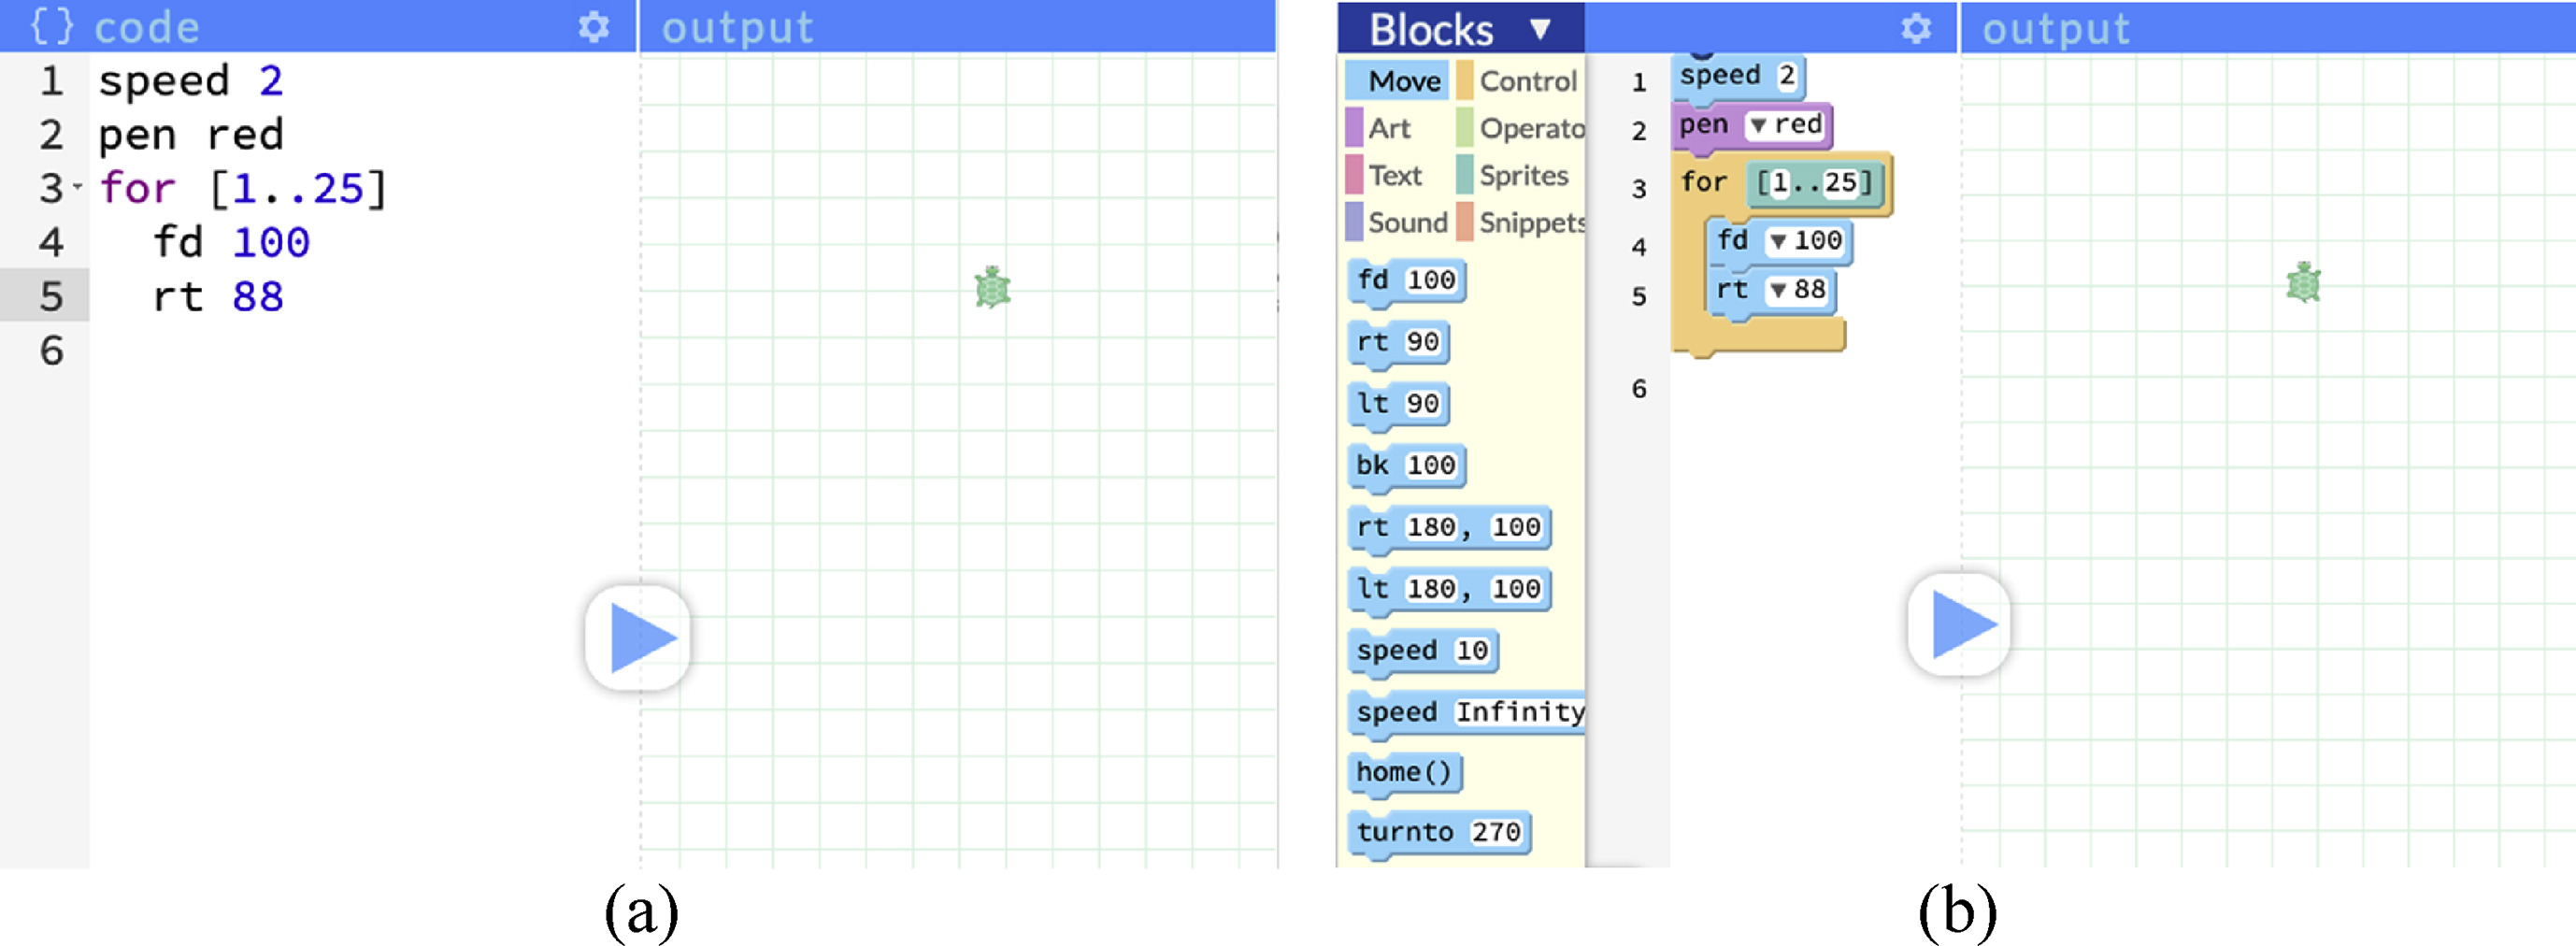
\includegraphics[width=0.9\textwidth]{Files/Billeder: Analyse/Pencilcc.jpg}
    \end{center}
    \caption{The two different approaches of the language of pencil.cc with the text-based in the left and block-based in the right \cite{FromBlockToText}.}
    \label{PA:pencilccFig}
\end{figure}

After five weeks both classes switched to learning the same text-based programming language Java. During the process, three tests were conducted, one before and after the introduction course and one after 10 weeks of learning Java. The outcome of the study is displayed in table \ref{tab:PB_A:LearningTest}. 

\begin{table}[H]
\resizebox{\textwidth}{!}{%
\begin{tabular}{|l|l|l|}
\hline
\textbf{} & \textbf{Block-based class} & \textbf{Text-based class} \\ \hline
\textbf{Test score before the learning course} & 54.3\% & 51.7\% \\ \hline
\textbf{Test score before starting the learning course} & 66.6\% & 58.8\% \\ \hline
\textbf{Test score learning Java} & 64.9\% & 65.7\% \\ \hline
\end{tabular}%
}
\caption{Overview of the average test result for the two different high school classes \cite{FromBlockToText}.}
\label{tab:PB_A:LearningTest}
\end{table}

\noindent
Table \ref{tab:PB_A:LearningTest} displays the result, it shows that the two classes were very similar in their prior programming knowledge. After the five-week introduction course, the class that followed the block-based version did significantly better. However, even though they gained a better understanding at first and scored higher on the mid-term test, the result of the last test was considered equal between the two classes. Besides the three tests that were conducted, data on their compilations were collected and reviewed. Like the test result, there was not any particular difference to find between the two classes \cite{FromBlockToText}. \\

Based on the result of the study \cite{FromBlockToText} and personal experiences of transitioning from block-based to text-based programming, using a block-based approach as an introduction to programming is simple and more intuitive for a new programmer, compared to the text-based approach. However, when switching from block-based to text-based programming, the same sense of difficulty and the same mistakes appear as for those that were introduced to programming through a text-based approach \cite{FromBlockToText}.\\

In view of the demand for new beginner programming languages, it is interesting to analyze and evaluate the differences between block-based and text-based programming. The analysis should illuminate the positive and negative aspects of text-based and block-based languages with beginner programmers as the target group.

\section{Analysis of Related Programming Languages} \label{subsection2.3}
To gain an insight into the difference between block-based and text-based languages, these will be evaluated using Sebesta's criterion, which is relevant when examining features in programming languages.\\ 

The analysis begins with the block language scratch in section \ref{section:AnalysisBlockBasesLanguages}. Furthermore, analysis and evaluation of text-based programming languages, including C, Python, and Quorum, in section \ref{text-basedlanguages}. The reasoning behind those specific languages being analyzed will be further elaborated in the following sections. \\

The languages are examined in terms of how they perform across Sebesta's criteria based on their readability, writability, and reliability. Furthermore, to identify their advantages and disadvantages for new programmers. Each criterion is further subdivided into several factors that contribute to the overall evaluation of a programming language as displayed in figure \ref{sebesta_criteria_table}. All the information upon Sebesta's criteria in this report is based on the book "Concepts of Programming languages" \cite{conceptsofproglang}. \\

\begin{figure}[H] 
    \begin{center}
        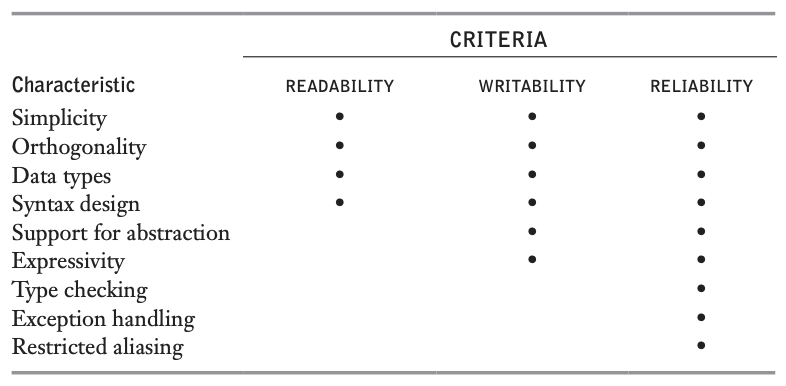
\includegraphics[width=0.9\textwidth]{Files/Billeder: Analyse/SebestaCriteria.png}
    \end{center}
    \caption{Language Evaluation Criteria and the Characteristics that affect them \cite{conceptsofproglang}.}
    \label{sebesta_criteria_table}
\end{figure}

%Figure \ref{sebesta_criteria_table} displays the three criterion: readability, writability, and reliability, and how they are effected by different factors. In the left side, the factors are listed.

\subsubsection{Readability}
Readability refers to how easy it is to read and understand code written in a particular programming language. A language that is highly readable will be easy to understand, debug, and maintain. Factors that affect readability include syntax clarity, ease of comprehension, and consistency of style \cite{conceptsofproglang}.

\subsubsection{Writability}
Writability refers to how easy it is to write code in a particular programming language. A language that is highly writable will be efficient for programmers to use, reducing development time and effort. Factors that affect writability include syntax simplicity, ease of expressing algorithms, and flexibility of control structures \cite{conceptsofproglang}.

\subsubsection{Reliability}
Reliability refers to how likely a program written in a particular programming language is to function correctly and consistently under different circumstances. A language that is highly reliable will produce fewer errors and bugs, resulting in more robust and stable programs. Factors that affect reliability include type checking, error handling, and exception handling \cite{conceptsofproglang}.

\subsection{Analysis of Scratch} \label{section:AnalysisBlockBasesLanguages}
Scratch is a Block-based programming language, which is a type of programming language that uses graphical blocks instead of traditional text-based code. These blocks represent programming concepts such as loops, conditional statements, and functions, and are typically arranged on the screen by dragging and dropping them into place. Some other popular block-based programming languages include Blockly and Code.org's App Lab \cite{popularblockbased}. Scratch is chosen because it is very popular and widely used in education, as it was developed to help children learn and express themselves through writing code. Scratch had 82 million users in December 2021, over 638 million projects created, and is the world's largest coding community for kids \cite{Scratchpopular}.\\

Scratch is a coding language with a simple visual interface \cite{scratchabout}. Scratch creates a visual environment for programmers which relies on the drag-and-drop method of programming. The different applicable components are structured in blocks with color coordination similar to LEGO blocks, as seen in figure \ref{fig:scratchexample}.\\

\begin{figure}[H] 
    \begin{center}
        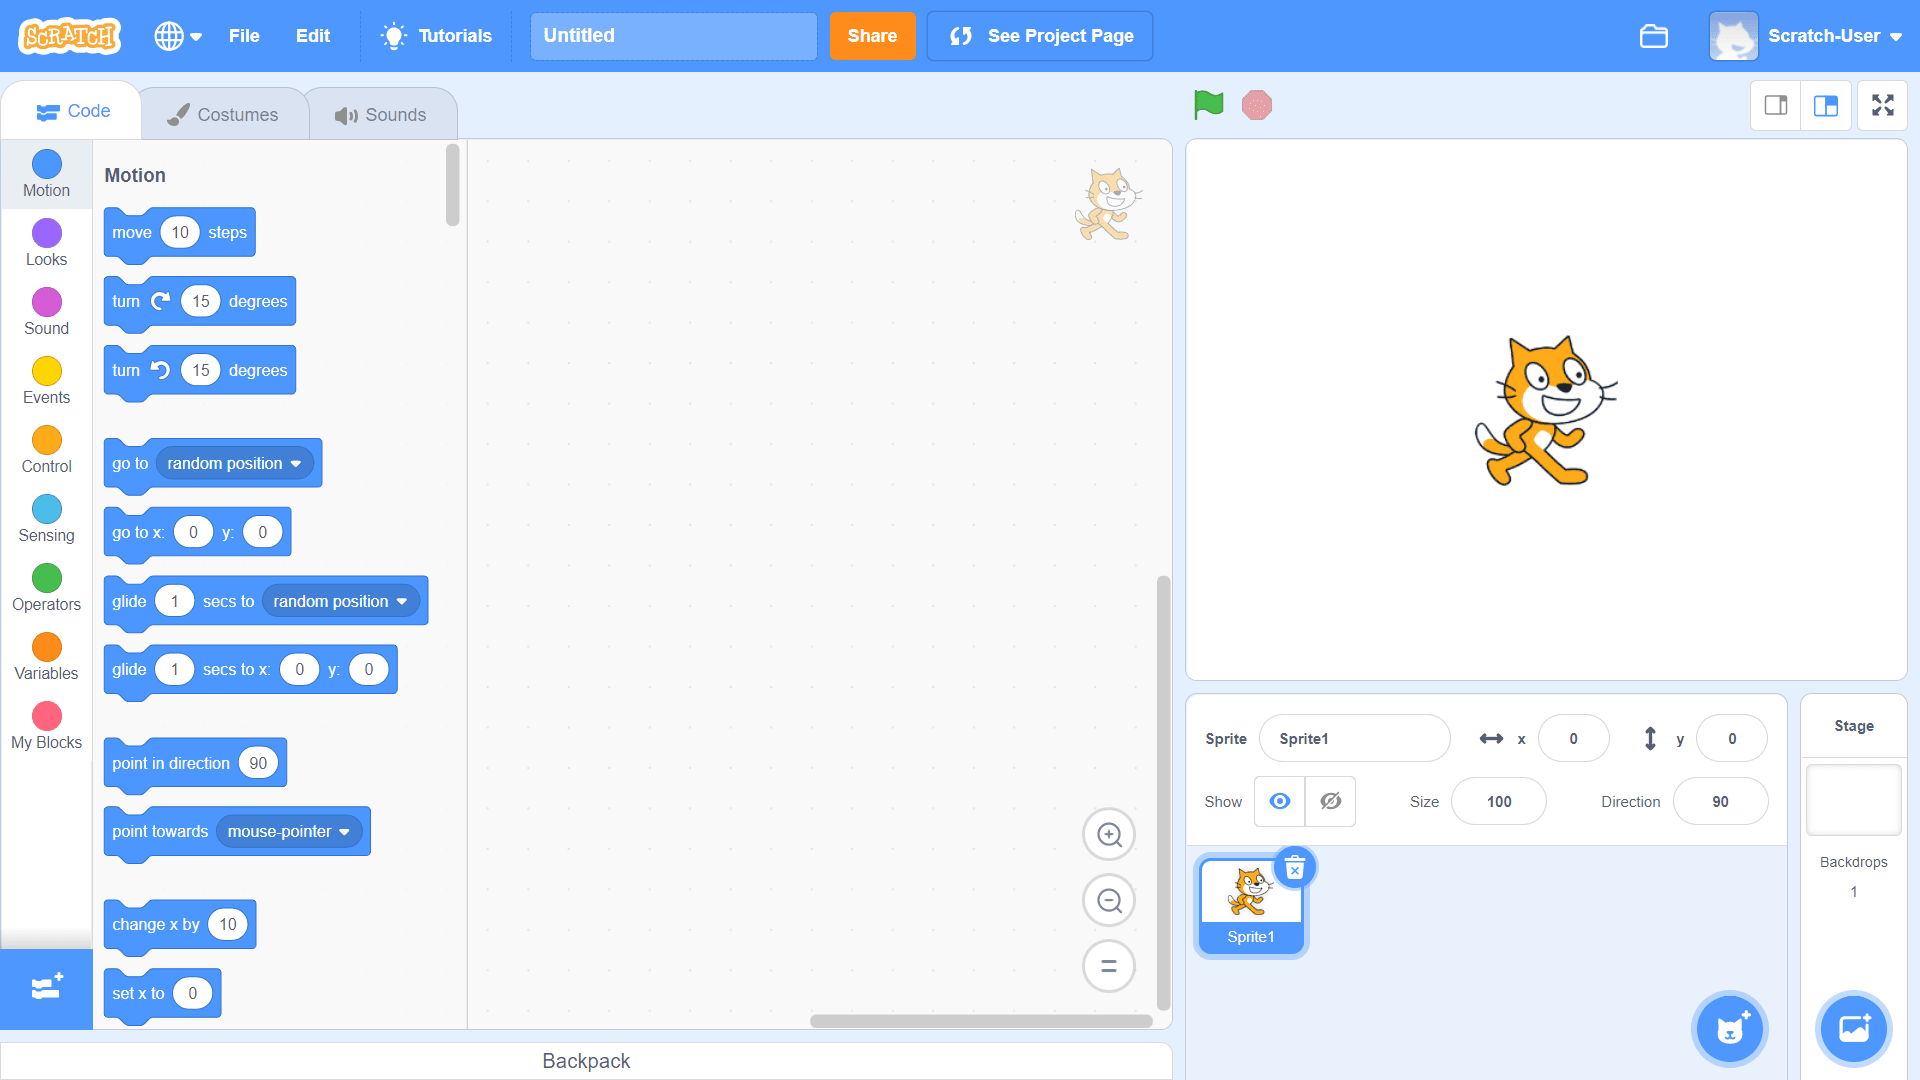
\includegraphics[width=0.9\textwidth]{Files/Billeder: Analyse/Scratch_3.0_Program.png}
    \end{center}
    \caption{Scratch Example \cite{ScratchEksempelBillede}.}
    \label{fig:scratchexample}
\end{figure}

%Blockly and code.org's App lab are similar to Scratch as they also provide a visual output of the programs as they are being developed through drag-and-drop block-based coding. They were chosen in this analysis as they are also a popular representation of the block-based programming languages \cite{popularblockbased}.

Scratch and other block-based languages, however, also have limitations in regard to their complexity. It cuts down on a lot of essential features that many of the popular text-based programming languages provide. This leads to a limited syntax, which makes it difficult to produce complex applications. The limited portability and scalability of block-based languages underline their purpose and target audience. It is clear from this that block-based languages are not intended to be widely used in the industry, but rather as a form of introduction to programming. \\

\noindent
If we take a look at Scratch in relation to Sebesta's Criteria in table \ref{sebesta_criteria_table}, the following analysis can be derived.\\

\noindent\textbf{Simplicity \& Orthogonality}\\
\noindent A language like Scratch is designed with learning in mind. Simplicity and orthogonality are very relevant when discussing block-based languages. Although Scratch is more focused on new programmers, it also has capabilities that an advanced programmer would use, including mutations of blocks or using component collections.\\

Simplicity \& Orthogonality have a special relation to mutation. A block with mutation(s) can be used in two ways. Beginner programmers can use blocks without mutations easily, while advanced users benefit from the optional parameters of the block.\\

In regards to abstract programming, component collection can be used when you want to set the width property of every button in a screen, instead of setting the property for the buttons one by one. This leads to a higher abstraction level of planning and development.\\

\noindent\textbf{Data types}\\
\noindent Scratch is very simple, and therefore only provides the basic data types such as string, number, and boolean. This also means that there are no subtypes in Scratch, such as integers or chars. This design consideration certainly simplifies the beginning phases of learning programming, since there are not multiple different ways to store a number. Still, the developer receives a core understanding of what data types are and will benefit from it if they pursue a lower-level language later on.\\

\noindent\textbf{Syntax Design}\\
\noindent The block groups have different colors and it is possible to play with the shapes of the blocks related to their different stacking and embedding types. This means that each block can contain different kinds of function block shapes e.g. a number that is a rectangle with rounded corners fits inside a "change x by *shape*" command block. These methods are very helpful for beginners in developing programs since they are given clues as to how to stack the blocks on top of each other. This usually benefits syntax considerations and avoids irritating "syntax error" messages.\\

\noindent\textbf{Support for abstraction}\\
Scratch has limited support for abstraction in the form of function definition. The programmer is able to create their own blocks and manipulate them to an extent. However, generalization of data types is not possible and it can be argued that the functions which can be created are restricted in their complexity. \\
% Most block-based languages are intended to support process abstraction, but it is also possible to find some data abstraction support, e.g. colors. Process abstraction is very important in block languages and the development method depends on the level of abstraction.\\


%What this means is that a higher level of process abstraction is a help for the beginner. As is the language, which is simple up to a specific level, since too many abstract processes could be confusing for a beginner.\\

\noindent\textbf{Expressivity}\\
\noindent Expressivity in Scratch is enhanced by the presence of powerful blocks that make it possible to accomplish a lot with a few blocks. This does mean that the programmer does not have full freedom in using these blocks, however, they do accelerate the learning process for beginners as they move towards the intermediate level. Apart from this, Scratch provides limited expressivity, as there in most cases are not multiple ways of accomplishing the same task. This is due to the blocks being specialized for specific purposes, taking away some freedom from the programmer while simplifying their use.\\

\noindent\textbf{Type checking}\\
\noindent 
Scratch performs type-checking to ensure that the blocks used in a script are compatible. In Scratch, the blocks are geometrically shaped to indicate their types, like in figure \ref{fig:scratchblocks}. For example, a boolean is shaped like a hexagon, and a rounded rectangle is for numbers or strings. By using these shapes, you are able to look at command blocks and the shapes they accept, to determine which kind of types you should make use of. This version of type-checking allows beginners to understand that there exist different types, which are not all interchangeable \cite{Scratchblocks}.

\begin{figure}[H]
    \begin{center}
        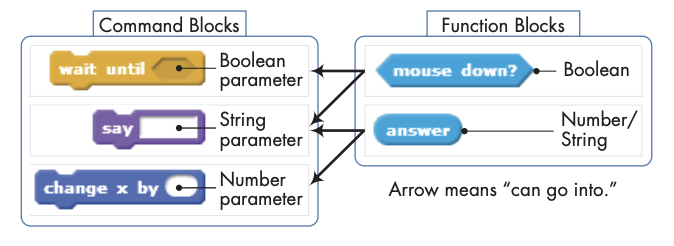
\includegraphics[width=0.75\textwidth]{Files/Billeder: Analyse/Scratchblocks.png}
    \end{center}
    \caption{Scratch blocks \& types \cite{Scratchblocks}.}
    \label{fig:scratchblocks}
\end{figure}

\noindent\textbf{Exception handling}\\
\noindent Exception handling is not usually an accessible feature of Block-based languages. There are no known statements on why exception handling is not an implemented feature within most block-based languages. However, it is fair to say Exception handling can be a complex concept for beginner programmers \cite{exceptionhandling}, and could therefore be the reason why it is not implemented. This means Scratch programs simply have to be error-free in order to run without crashing.\\

\newpage
\noindent\textbf{Restricted aliasing}\\
\noindent Since you are not able to have two or more distinct names in a block-based language that can access the same memory cell, as well as the lack of pointer implementation or a form of reference, Scratch does not have aliasing, and strict aliasing is not a relevant problem.\\

\noindent\textbf{Summary}\\
\noindent Block-based programming languages rely on graphical blocks instead of traditional text-based code, with Scratch being one of the most popular, with 82 million users and over 638 million projects created. Other popular block-based programming languages include Blockly and Code.org's App Lab. The simplicity and orthogonality of Scratch make it an excellent language for new programmers to learn. However, this simplicity also means Scratch is limited in terms of complexity, making it difficult to produce complex applications. The text also provides an analysis of Scratch in relation to Sebesta's Evaluation Criteria, discussing its simplicity, data types, syntax design, support for abstraction, and expressivity. Overall, Scratch is an excellent language for teaching basic coding concepts to children and beginners, but may not be suitable for developing more advanced applications.

\subsection{Analysis of relevant text-based programming languages} \label{text-basedlanguages}
%Widely used in the industry
%Beginner friendly (Often used by beginners)
%A "hard", widely used language, in order to compare the differences between easy and hard
%Quorum has been chosen because it is evidence based, and also focuses on teaching programming.

%A relevant language, in this case, is defined as a language often used by beginners as their introductory language, or a language widely used in the industry. 

In section \ref{SelectionLang}, three text-based programming languages are analyzed. In order to select more relevant languages to analyze, considering programming paradigms is appropriate.

\subsubsection{Programming Paradigms}
Programming paradigms help categorize different styles of programming and can be used to describe a programming language. Some of the most commonly used programming paradigms include 'imperative' and 'declarative'. The imperative programming paradigm is a way of programming where the instructions given are used to change between states. Each instruction given, like changing the contents of a variable, represents a state change \cite{WikiProgrammingParadigms}. Examples of this are C, Java, and C\#. \\
In the declarative programming paradigm, no instructions regarding how to compute anything are given, rather the properties of the needed result are given and the underlying required computations are made based on this result \cite{WikiProgrammingParadigms}. Examples of this are most database query languages like SQL. Because many paradigms are similar and/or derive from other paradigms, most programming languages are considered to be multi-paradigms.\\ 

\newpage \noindent
\textbf{Procedural programming:} Within the imperative- and declarative programming paradigm are subcategories. Both 'procedural' and 'object-oriented' are subcategories of imperative programming. The procedural paradigm is about changing states using procedures/subroutines. Procedures are functions with the purpose of changing the value of their arguments and they do not return an output. Most procedural languages are also imperative but the main difference is that the procedural paradigm depends on scopes and therefore most languages containing control structures like \textit{for}, \textit{while} and \textit{if} are procedural \cite{WikiProgrammingParadigms}. A language without scopes that instead use for example 'goto' would be considered imperative but not procedural. C, Java, and C\# are also considered procedural programming languages. \\
%https://en.wikipedia.org/wiki/Procedural_programming

\noindent
\textbf{Object-oriented programming:} Instead of changing states through procedures, the object-oriented paradigm changes states through its objects which themselves can contain procedures and functions. In this way, they are similar to the procedural paradigm, and usually, an object-oriented programming language is also considered procedural as it supports procedures and sequences of instructions \cite{WikiProgrammingParadigms}. Examples include Java and C\#. \\
%https://en.wikipedia.org/wiki/Procedural_programming

\noindent
\textbf{Functional programming:} The most notable subcategory within declarative programming is functional programming. In functional programming, the result wanted by the user is defined using a series of functions \cite{FunctionalProgrammingParadigm}. In the functional paradigm, a function cannot contain side effects, meaning that any input is mapped directly to an output. There do not exist popular purely functional programming languages, though some languages like C\# include features from the functional paradigm with their use of LINQ and lambda expressions \cite{FunctionalProgrammingParadigm}. \\
%https://en.wikipedia.org/wiki/Functional_programming

\subsection{Selecting the languages} \label{SelectionLang}
The languages will be from the imperative programming paradigm, including the paradigms: procedural and Object-oriented, as languages in these paradigms, are easy to learn and read, compared to languages from the declarative paradigm \cite{ProgrammingParadigme}.\\

When considering the selection of languages to analyze within the imperative paradigm, Python, Quorum, and C is chosen based on the following arguments:

Python is chosen because it has a simple syntax \cite{PythonLanguageReference}, is widely used in the industry \cite{TopProgrammingLanguages2022}, and is a common starting language for new programmers \cite{PythonBeginnerProgrammingLanguage}. \\

Quorum is interesting to analyze because it is used as an introductory language, e.g. in high schools. It has a simple and readable language design \cite{QuorumVid}. Furthermore, Quorum is an evidence-based language meaning that it was developed based on the results of scientific research in order to improve its language design \cite{QuorumProgLang}.\\

C is selected because it is widely used in the industry \cite{5ReasonsForC}, and because it is the predecessor for many other widely used languages such as Python, Java, and C\#. This can be seen in figure \ref{Prog_Lang_Tree}. C and Python are circled to indicate their presence in the tree, and the red lines indicate the connection between C and the other mentioned languages. However, C is viewed as a less beginner-friendly language, as it has constructs such as pointers, dynamic memory allocation, etc, which can be hard to grasp for new programmers \cite{5ReasonsForC}. 

\begin{figure}[H] 
    \begin{center}
        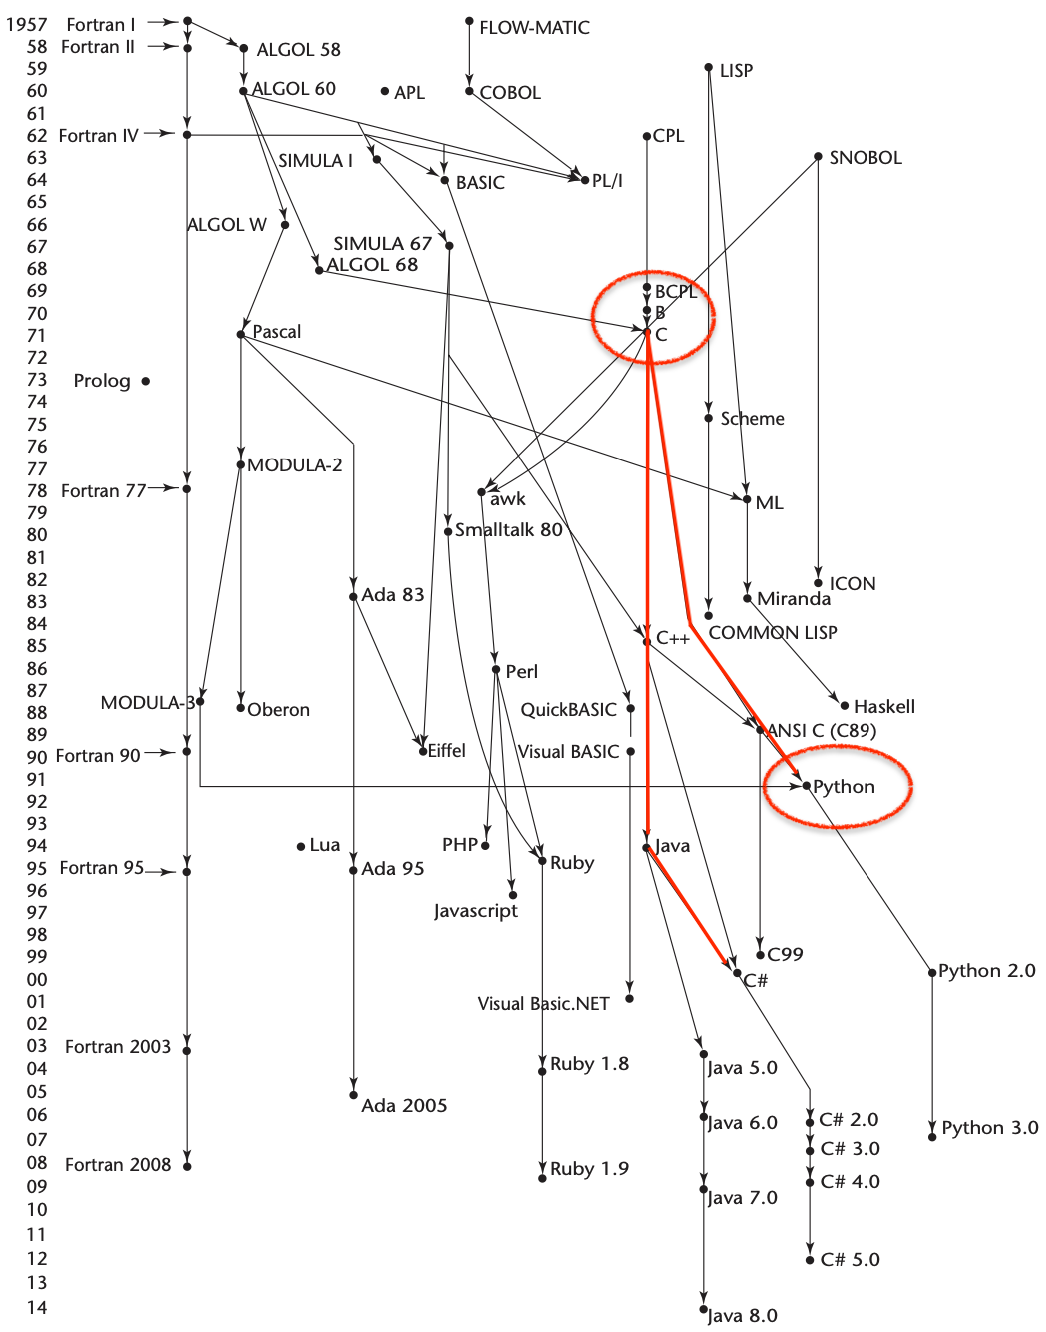
\includegraphics[width=0.9\textwidth]{Files/Billeder: Analyse/ProgTree.png}
    \end{center}
    \caption{A programming language evolution tree. \cite{conceptsofproglang}.}
    \label{Prog_Lang_Tree}
\end{figure}

\newpage
\subsubsection{Python Language}
Python is an object-oriented programming language with a simple syntax. Python supports multiple programming paradigms such as procedural and functional programming \cite{PythonLanguageReference}. The Python programming language is considered a high-level text-based programming language. With an easy and English-like syntax, Python is considered a beginner-friendly language \cite{PythonGoodForBegin}. An example of a small Python program can be seen in figure \ref{codeEx:Python}\\

\begin{figure}[H] 
    \begin{center}
        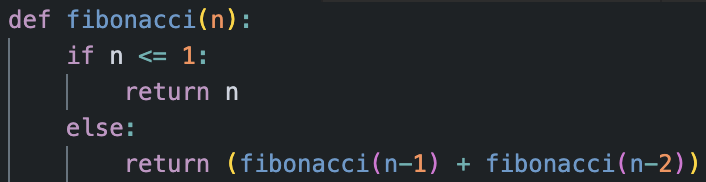
\includegraphics[width=0.9\textwidth]{Files/Billeder: Analyse/PythonFiboExample.png}
    \end{center}
    \caption{Python Fibonacci Example.}
    \label{codeEx:Python}
\end{figure}

\noindent\textbf{Simplicity}\\
\noindent In Python few lines can amount to larger functionalities. Due to this, some concepts can be easy to learn and read while others can seem cryptic. Python's short syntax makes it easier to write code, improving writability overall.\\

\noindent\textbf{Orthogonality}\\
\noindent Python has a high degree of orthogonality. This means that the constructs in the language can be combined in multiple ways which initially makes Python easier to read and write \cite{progEvalArticle}. However, having very high orthogonality might be a disadvantage, as it then allows very complex constructs due to combinatorial freedom.
\\

\noindent\textbf{Data types}\\
\noindent Python has multiple built-in data types, such as integers, strings, and floats, but it also supports more complex data types such as lists, etc. With many built-in data types, expressivity is improved. However, there are some downsides to having a lot of built-in data types, one of which is making the language more complex and harder to learn.\\

\noindent\textbf{Syntax design}\\
\noindent Pythons syntax is short and readable \cite{PyntaxSyntax}, which helps improve readability and writability. Python syntax uses indentation instead of curly brackets as scopes, which for some users makes the code more readable, whereas it can cause confusion for others who are used to curly brackets.\\

\noindent\textbf{Support for abstraction}\\
\noindent Python includes support for abstraction by letting the programmers define their own functions and classes and such. By having support for abstraction, writability is increased as it allows some functionality to be reused later on.\\

\noindent\textbf{Expressivity}\\
\noindent Python has high expressivity. This is due to the fact that Python allows its programmers to express ideas in multiple different ways, each with their own advantages. Expressivity can improve readability and writability. However, high expressivity may also make the language harder to read for some, as too many ways of expressing the same functionality may cause confusion. The programmer has to keep track of a larger collection of constructs in order to fully utilize the functionality of the language.\\

\noindent\textbf{Type checking}\\
\noindent Python is a dynamically typed language, which means that the interpreter assigns variables a type at runtime based on the variable's value at the time \cite{Dynamic_Typing}. By being a dynamically typed language Python becomes more flexible. It can also lead to some type-related errors which may be difficult to catch during development. However, Python is at the same time strongly typed, meaning that variables have a type and that it matters when performing operations on the variable.\\

\noindent\textbf{Exception handling}\\
\noindent Python has support for exception handling. This makes it easier to develop code that can handle errors, which can help improve reliability by handling errors, which are expected to occur.\\

\noindent\textbf{Restricted aliasing}\\
\noindent Python does not have restricted aliasing. This slightly lowers the reliability of the language compared to languages that support it.

% Python has restricted aliasing. This improves reliability by having some unexpected changes due to changes to some of the shared data that can happen with aliasing.\\


\noindent\subsubsection{Quorum Language}
\noindent Quorum is a high-level programming language, which is intended mainly for students but is broad enough to also be used commercially \cite{QuorumProgLang}. One of the main focuses of the language is for its syntax to be simple and accessible because it is meant to be easy to learn for all types of learners. Furthermore, it aims to improve language design overall \cite{QuorumVid}. An example of a small Quorum program can be seen in figure \ref{codeEx:Quorum}\\

\begin{figure}[H] 
    \begin{center}
        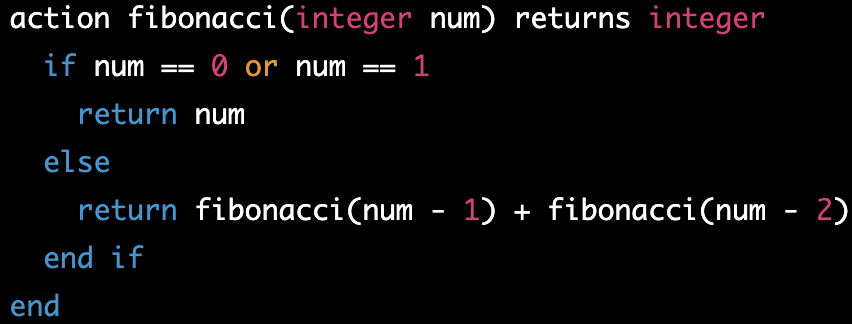
\includegraphics[width=0.9\textwidth]{Files/Billeder: Analyse/QuorumFiboExample.png}
    \end{center}
    \caption{Quorum Fibonacci Example.}
    \label{codeEx:Quorum}
\end{figure}

\noindent\textbf{Simplicity}\\
\noindent Since quorum is designed to be simple and easy to learn, its syntax is straightforward and easy to read, which enhances its readability. Its simplicity also enhances the language's writability. Finally, Quorum's simple design helps to reduce the potential for errors, which enhances its reliability.\\

\noindent\textbf{Orthogonality}\\
\noindent Quorum supports a relatively small set of primitive constructs that can be combined in a variety of ways to build control and data structures. This orthogonality helps to make the language easy to learn and use, which enhances readability and writability. Additionally, orthogonality increases the reliability of code written in the language.\\

\noindent\textbf{Data types}\\
\noindent The data types supported by Quorum include integers, booleans, strings, and arrays. The use of clear and consistent data types enhances Quorum's readability and writability, as it is easy to understand the purpose and behavior of different data types. Furthermore, the use of strong typing and type-checking mechanisms helps to improve the reliability of code written in the language.\\

\noindent\textbf{Syntax design}\\
\noindent Quorum's syntax is designed to be simple and clear, which enhances its readability. The use of consistent and intuitive syntax design also helps to improve the language's writability, as developers can easily understand how to use different language constructs. However, writability is not as high as it could be, since the syntax in many cases, forces the developer to write the full name of a construct, e.g. "boolean", instead of "bool", as booleans are called in some programming languages. Having to write the full-length construct names instead of an abbreviation, increases readability, but reduces writability, as the programmer would be able to write a program faster using abbreviations for the constructs. Finally, the use of a clear syntax design improves the reliability of code written in the language.\\

\noindent\textbf{Support for abstraction}\\
\noindent Quorum includes support for abstraction, in the form of object-oriented features such as inheritance and encapsulation. This helps improve writability and reliability, as the developer is able to write reusable code that is easy to modify and maintain.\\

\noindent\textbf{Expressivity}\\
\noindent Quorum low expressivity as it does not have many ways of expressing the same computations. For example, the count++ notation from C and other languages does not exist in Quorum, where the only way of counting up a variable is "count = count + 1". An example where Quorum contains constructs that can specify the same computation is with its loops. Quorum has three types of loops: Repeat x times, repeat until, and repeat while. Repeating x times makes it easy to repeat the same action a specific amount of times. However, repeat until and repeat while can also be used for the same purpose, but are more powerful, as they both run based on a boolean condition. By itself, the quorum language does not have very high expressivity, however, this changes with its different libraries, which simplify many different actions. Expressivity enhances the language's readability and writability, and developers can use language constructs that are intuitive and easy to understand.\\

\noindent\textbf{Type checking}\\
\noindent Quorum is statically typed and includes strong type-checking mechanisms, which help to improve the reliability of code written in it. Type checking helps to ensure that code is correct and free from errors related to data types.\\ 


\noindent\textbf{Exception handling}\\
\noindent Quorum includes support for exception handling by the programmer, which helps to improve the reliability of code written in the language. The error handling in Quorum allows the use of a Try-Catch-Finally statement, however, the syntax is different, as Quorum uses a check-detect-always syntax instead. \\


\noindent \textbf{Restricted aliasing}\\
\noindent Quorum does not include support for restricted aliasing, which slightly lowers the reliability of the language compared to languages that support it.
% Quorum includes support for restricted aliasing, which helps to prevent errors related to data aliasing. This enhances the language's reliability, as it helps to prevent errors that can be difficult to detect. \\


\subsubsection{C Language}
C is an imperative text-based programming language that is considered low-level compared to other more popular languages like Python or C\#\cite{WikiCLang}. It is widely used due to its lower level, making it an efficient language for writing code closely linked to machine instructions. One way that C is considered low level is for example its inclusion of pointers, which can point to an address in memory, similarly to machine instructions in assembly\cite{WikiCLang}. An example of a small C program can be seen in figure \ref{codeEx:C}
%https://en.wikipedia.org/wiki/C_(programming_language)

\begin{figure}[H] 
    \begin{center}
        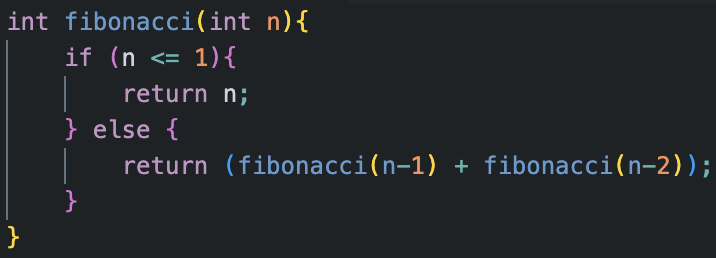
\includegraphics[width=0.75\textwidth]{Files/Billeder: Analyse/CFiboExample.png}
    \end{center}
    \caption{C Fibonacci Example.}
    \label{codeEx:C}
\end{figure}


\noindent\textbf{Simplicity}\\
\noindent C has a limited amount of data types and keywords making it simple, however, some instructions, which in other languages require one line, may require multiple lines in C. An example of this is C's lack of built-in properties like arrays ".length" property which exists in most languages. An arrays length can be accessed any time through the array in C\# and Python, while in c you would have to initialize the array and calculate the length of the array on separate lines. The language also requires some knowledge of low-level programming because of its inclusion of concepts like pointers and dynamic memory allocation. \\

\noindent\textbf{Orthogonality}\\
\noindent C does not include higher-level components such as lists, but combining the components that are included can create more advanced structures. In C, certain operators cannot be used on some data types which are otherwise possible in some higher-level languages like C\#. For example in C strings cannot be concatenated using "+".\\

\noindent\textbf{Data types}\\
\noindent In C there are a limited amount of data types. Today most languages include data types like "bool" and "string". In C, "true" is represented by any integer value that is not 0, and to make a string, an array of characters is needed. \\

\noindent\textbf{Syntax Design}\\
\noindent Some of the syntax in C can be considered hard to learn for beginners such as pointers and indirect component selection of struct fields. Many words are reserved and have special meanings in C. The only keyword which violates this is the keyword "static" which can be used to declare global variables within a scope, or used to define that an array parameter needs a specific length.\\

\noindent\textbf{Support for Abstraction}\\
\noindent In C, the programmer is able to create abstraction by using functions and structs. These abstractions can be considered low compared to higher-level languages which include classes, inheritance, and dynamic objects.\\

\noindent\textbf{Expressivity}\\
\noindent In higher-level languages the programmer is able to have more functionality on fewer lines than in C. Despite this, code can be written concisely in C though it may be hard to read.\\

\noindent\textbf{Type Checking}\\
\noindent C contains limited methods of type checking. C allows implicit typing, making detecting errors difficult\\

\noindent\textbf{Exception Handling}\\
\noindent C does not have built-in exception handling like other higher-level languages. For example, Quorum and Python have a try-catch structure and the ability to throw an error, like previously mentioned in their analysis. "Try-catch" and throwing an error is not possible in C\\

\noindent\textbf{Restricted aliasing}\\
\noindent C has "restricted pointers" which helps express anti-aliasing in C but besides this, C's heavy need for pointers when making functionality, makes aliasing occur often in the language. The restrict keyword on a pointer is a way of telling the compiler that the specific pointer is the only way of accessing the object pointed by it \\

\subsection{Comparing languages} \label{ComparingLanguages}
In this section, a comparison between the languages previously analyzed in section \ref{subsection2.3} is conducted. These languages will be compared based on their overall readability, writability, and reliability in order to understand the difference and deduct how a language aimed at beginners, compares to these languages. Each language is put on a scale ranging from low to high on readability, writability, and reliability. These scales represent how these language rank compared to each other based on the analysis.

\newpage
\subsubsection{Comparing readability}
First up is comparing readability. The languages are ranked on the scale,  displayed in figure \ref{PA:readability_scale}. 

\begin{figure}[H] 
    \begin{center}
        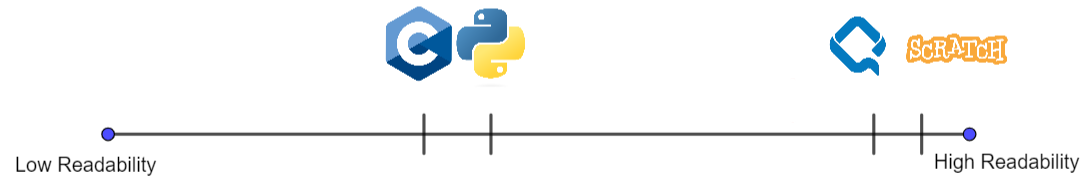
\includegraphics[width=0.9\textwidth]{Files/Billeder: Analyse/Readability.png}
    \end{center}
    \caption{The programming languages C, Python, Quorum, and Scratch placed on a scale showing readability.}
    \label{PA:readability_scale}
\end{figure}

C has the lowest readability of the languages that have been analyzed in figure \ref{PA:readability_scale}. This is due to the fact that it is a low-level programming language, in which a line of code often closely resembles machine instructions. The main reason for not placing C lower on the readability scale is due to the fact that languages such as Assembly have notably lower readability. \\

Next on the scale in figure \ref{PA:readability_scale} is Python which has better readability. The reason is that Python focuses a lot more on writability which will be elaborated on in figure \ref{PA:writability_scale}. In Python, the programmer is able to write readable code for intermediate programmers while also having the ability to write a lot of functionality within a few lines which may be confusing for beginner programmers.\\

The next language on the scale in figure \ref{PA:readability_scale} is Quorum. Quorum has been placed high on the readability scale. This is due to the fact that Quorum has a simple syntax, which focuses on readability over writability. Compared to a language like Python where the programmer is able to write flexible code with a focus on writability and less readability, there is less room for complex code in Quorum as it focuses on simplicity.\\

Scratch has high simplicity which makes it more beginner friendly and readable. Every block is labeled in order to remove ambiguity in the language (see figure \ref{fig:scratchexample}). Coding larger functionalities in Scratch could be considered confusing for beginners, due to the large amount of blocks which can be combined, but despite this, the blocks still help define the functionalities.\\

\subsubsection{Comparing writability}
Next, is comparing the writability. The languages is ranked on the scale,  displayed in figure \ref{PA:readability_scale}. 

\begin{figure}[H] 
    \begin{center}
        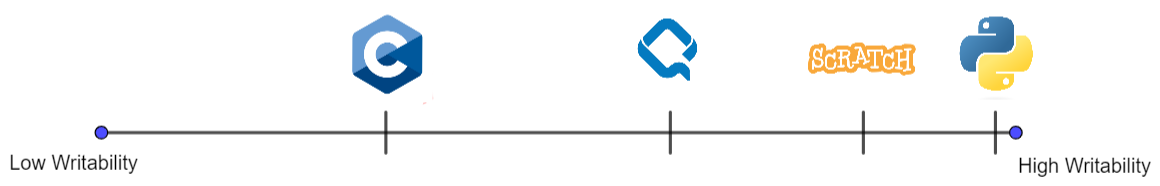
\includegraphics[width=0.9\textwidth]{Files/Billeder: Analyse/Writability.png}
    \end{center}
    \caption{The programming languages C, Python, Quorum, and Scratch placed on a scale showing writability.}
    \label{PA:writability_scale}
\end{figure}

The language with the lowest writability on the scale in figure \ref{PA:writability_scale} is C. One of the reasons for this is due to C being a low-level language and therefore has low expressivity. C does not contain many ways in which you can express complex concepts in a few lines. Compared to higher-level languages, C also has less support for abstraction like previously mentioned in the analysis. In general, C is very bare-bones and limited compared to other languages.\\

Quorum is placed in the on figure \ref{PA:writability_scale} regarding writability. Compared to C, it is more expressive and has more support for abstraction, for example in the form of its object-oriented features. Quorum is placed lower compared to Python and Scratch because of its need to be readable. For example, the data type "int" in C, is an abbreviation for "integer", which is the name used in Quorum.\\

In Scratch, each "block of code" has to be dragged in. This makes it simple to create code since all available code blocks can be seen in a sidebar. Scratch is placed lower on figure \ref{PA:writability_scale} than Python because despite how easy this is, Scratch has limited expressivity compared to Python where it may be faster to write code than looking for and dragging in multiple blocks.\\

Especially because of Python's high level of expressivity, a lot of functionality can be written in a few lines. Python is therefore placed highest on the scale in figure \ref{PA:writability_scale}. Python also has a lot of support for abstraction and orthogonality compared to C, Quorum, and Scratch.\\

\newpage
\subsubsection{Comparing reliability}
The last criterion that is compared is reliability. The languages are ranked and displayed in figure \ref{PA:reliability_scale}.

\begin{figure}[H] 
    \begin{center}
        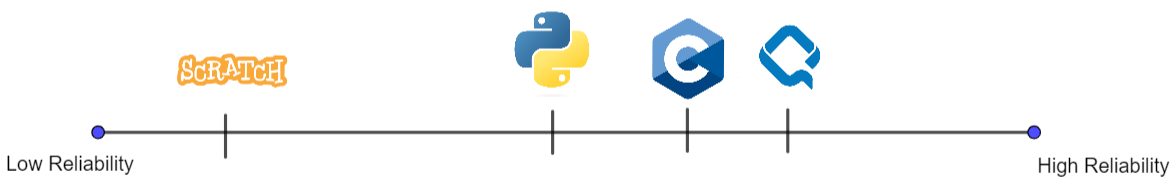
\includegraphics[width=0.9\textwidth]{Files/Billeder: Analyse/Reliability.png}
    \end{center}
    \caption{The programming languages C, Python, Quorum, and Scratch placed on a scale showing reliability.}
    \label{PA:reliability_scale}
\end{figure}

Scratch does not have exception handling and is dynamically typed. If the programmer decides to set the value of a variable equal to two strings added together, no error is displayed, and instead, the value becomes 0. This makes Scratch less reliable and Scratch is therefore placed lowest on the scale in figure \ref{PA:reliability_scale}, as the programmer is not warned about unwanted behavior. Scratch does have restricted aliasing making it slightly more reliable.\\

Python is dynamically and strongly typed and is able to for example interpret strings to numbers and vice versa, however, the programmer can get unwanted behavior when letting Python do automatic type conversion. Python still allows for explicit type conversion though. This gives Python lower reliability, ranked lower than C and Quorum on the scale in figure \ref{PA:reliability_scale}, but higher reliability than Scratch.\\

In C the programmer does not have access to exception handling, but C is statically typed making it more reliable than Python and Scratch in figure \ref{PA:reliability_scale}. C has limited support for restricted aliasing, but with its focus on using pointers, it does have aliasing.\\

Quorum provides exception handling for the programmer and is statically typed. This makes Quorum more reliable than the other languages analyzed. 

\begin{comment}
\subsection{Comparing languages}
In this section, a comparison between the languages previously analyzed in section \ref{subsection2.3} is made. These languages will be compared based on their overall readability, writability, and reliability in order to understand the difference and deduct where a language aimed at beginners, lies on the scales compared to other languages. The goal for the language is to be readable and understandable for beginners while also making the transition to other industry standards easier. Therefore the goal is to prioritize readability higher than writability while also making sure that it is somewhat reliable.

\subsubsection{Comparing readability}
The first language on the scale is C. C has the lowest readability of all the languages which have been analyzed. This is due to the fact that it is a low-level programming language, in which a line of code often closely resembles machine instructions. \\

Next on the scale is Python which has better readability. The reason is that Python focuses a lot better on writability which will be elaborated on in figure \ref{writability}. In Python, the programmer is able to write readable code while also having the ability to write a lot of functionality within a few lines which may be considered unreadable.\\

The next language on the scale is Quorum. Quorum has been placed high on the readability scale. This is due to the fact that Quorum has a simple syntax, which focuses on readability over writability. Compared to a language like Python where the programmer is able to write flexible code with a focus on writability and less readability, there is less room for complex code in Quorum as it focuses on simplicity.\\

Scratch has high simplicity which makes them more beginner friendly and readable. Every block is labeled in order to remove ambiguity in the language. Coding larger functionalities in Scratch could be considered confusing due to the large combination of blocks, but despite this, the blocks still help define the scopes clearly and concisely.\\

After analyzing these languages, and making some considerations about where on the scale, the language \lang should be placed, it has been decided that \lang should be very readable in order to help beginners. However, at the same time, it should also help new programmers with transitioning to some common industry standards. Because of this, \lang has been placed between Python and Quorum, but closer to Quorum. This is due to the focus on readability, as people who have not programmed before, should be able to recognize the constructs of \lang. This would help beginners learn the language quicker as well. Figure \ref{readability} visualizes a comparison of the language's readability on a simple scale. To simplify, block-based languages are represented by the Scratch programming language

\begin{figure}[H] 
    \begin{center}
        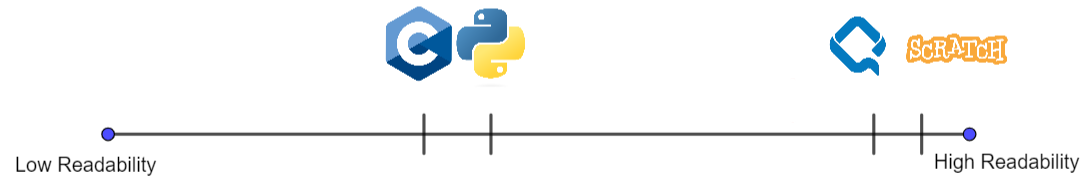
\includegraphics[width=0.9\textwidth]{Files/Billeder: Analyse/Readability.png}
    \end{center}
    \caption{The programming languages C, Python, Quorum, and Scratch placed on a scale showing readability. The red arrow indicates an assumption of where \lang lies on the scale}
    \label{readability}
\end{figure}

\subsubsection{Comparing writability}
The language with the lowest writability on the scale is C. One of the reasons for this is due to C being a low-level language and therefore has low expressivity. C does not contain many ways in which you can express complex concepts in a few lines. Compared to higher-level languages, C also has less support for abstraction. In general, C is very bare-bones and limited compared to other languages.\\

Quorum is placed in the middle regarding writability. Compared to C, it is more expressive and has more support for abstraction, for example in the form of its object-oriented features. Quorum is placed lower compared to Python and Scratch because of its need to be readable. For example, the data type "int" in C, is an abbreviation for "integer", which is the name used in Quorum.\\

In Scratch, each "block of code" has to be dragged in. This makes it simple to create code since all available code blocks can be seen in a sidebar. Scratch is placed lower than Python because despite how easy this is, Scratch has limited expressivity compared to Python where it may be faster to write code than looking for and dragging in multiple blocks.\\

Especially because of Python's high level of expressivity, a lot of functionality can be written in a few lines. Python also has a lot of support for abstraction and orthogonality compared to C, Quorum, and \lang.\\

\lang has been placed between C and Quorum, but closer to C. This is due to the fact that the language will have low expressivity, limited support for abstraction (no object-oriented constructs), and a limited amount of data types. Like Quorum, the goal of this language is to focus more on readability in preference to writability. Also like Quorum, the focus will be for beginners to be able to quickly recognize and understand the language, and therefore most reserved keywords will not be abbreviations like in many languages.

\begin{figure}[H] 
    \begin{center}
        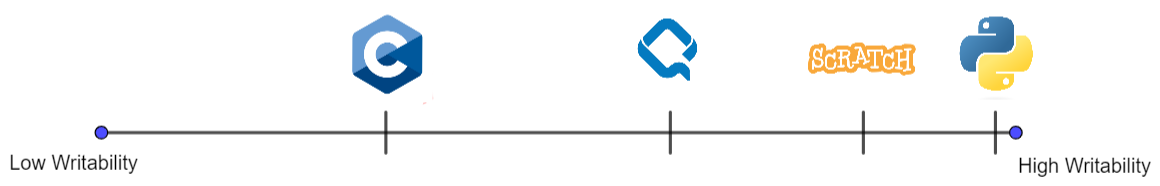
\includegraphics[width=0.9\textwidth]{Files/Billeder: Analyse/Writability.png}
    \end{center}
    \caption{The programming languages C, Python, Quorum, and Scratch placed on a scale showing writability. The red arrow indicates an assumption of where \lang lies on the scale}
    \label{writability}
\end{figure}

\subsubsection{Comparing reliability}
Scratch does not have exception handling and is dynamically typed. If the programmer decides to set the value of a variable equal to two strings added together, no error is displayed, and instead, the value becomes 0. This makes Scratch less reliable, as the programmer is not warned about unwanted behavior. Scratch does have restricted aliasing making it slightly more reliable.\\

Python is dynamically and strongly typed, and is able to for example interpret strings to numbers and vice versa, however, the programmer can get unwanted behavior when letting Python do automatic type conversion. Python still allows for explicit type conversion though. This gives Python lower reliability than other languages on the list, but higher reliability than Scratch.\\

In C the programmer does not have access to exception handling, but C is statically typed making it more reliable than Python and Scratch. C has limited support for restricted aliasing, but with its focus on using pointers, it does have aliasing.\\

Quorum provides exception handling for the programmer and is statically typed. This makes Quorum more reliable. Quorum is also placed more left than C because despite it having aliasing like C, C focuses a lot on pointers which is not included in Quorum. \\

\lang is being placed between C and Quorum on this scale. This is because the language will not include exception handling, as this is not a necessary tool for beginners in programming. To avoid type conversion errors, the language will be statically typed and have type-checking in order to avoid confusion for new programmers. The language will have limited or restricted aliasing, as references are a more advanced concept.

\begin{figure}[H] 
    \begin{center}
        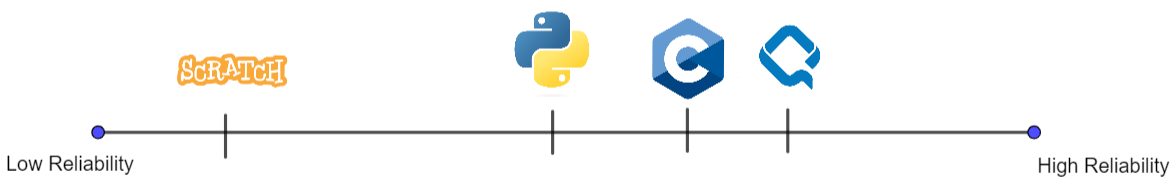
\includegraphics[width=0.9\textwidth]{Files/Billeder: Analyse/Reliability.png}
    \end{center}
    \caption{The programming languages C, Python, Quorum, and Scratch placed on a scale showing reliability. The red arrow indicates an assumption of where \lang lies on the scale}
    \label{reliability}
\end{figure}
\end{comment}

\section{Summary}

To summarize, The languages above are compared based on their ability to be understood by beginners, written in a straightforward way, and produce the desired output without errors. The analysis shows that C has the lowest readability and writability, while Python has high expressivity, which makes it easier to write code. Quorum focuses on readability over writability, making it more beginner-friendly. Scratch is also beginner-friendly but has limited expressivity. In terms of reliability, C is statically typed, which makes it more reliable than Python and Scratch. Quorum provides exception handling and is also statically typed, making it more reliable than C. C lacks exception handling, making it less reliable than Quorum.

\section{Problem statement} \label{problemstatement}
%From the analysis, a gap between the current existing languages can be seen. Based on the fact that many beginner programmers find it difficult to transition from any block-based language to some of the industry standard languages, a need for a language that can be used to handle this transition is needed. \\

%\noindent From this the following problem statement can be derived. \\ \\
%\noindent \textit{Explain and display a text-based programming language, which is aimed towards transitioning beginner programmers into using industry standard programming languages.}

From the analysis, a vacancy between the existing languages can be seen. As a beginner programmer, there are several ways to learn to program. Learning to program in a block-based language is widely used and tends to be a positive way to evolve computational thinking and be introduced to programming. But despite this, beginner programmers find it difficult to transition from a block-based language to some of the industry standard languages. The introduction to a text-based programming language is challenging and requires persistence. \\
Based on the analysis and comparison of the four different languages there are different pros and cons seen from a beginner's perspective. By the conclusion of the analysis, the goal of our language is a beginner-friendly text-based language that is developed to introduce beginner programmers to the basic and important concepts in programming is needed. \\

From this, the following problem statement can be derived.

\begin{center}
    \textit{How can a text-based programming language be developed for beginner programmers, using readable concepts from block-based languages, while focusing on facilitating the transition to programming languages used in the industry?}
\end{center}

A list of requirements has been made in order to successfully be able to say, that the problem statement has been solved. The list has been made in chronological order, and the details, importance, and use will be presented throughout the report.

% \begin{itemize}
% %  \item Analyze beginner programmers.
%   \item Define language criteria for \lang.
% %  \item Explain the programming paradigm of \lang.
% %  \item Create a MoSCoW requirement table.
%   \item Create and explain the Context-Free Grammar (CFG) for \lang.
%   \item The creation of a lexer and parser.
%   \item Define semantics for \lang.
%   \item Abstract Syntax Tree (AST) design for \lang.
%   \item Definition of scope rules.
%   \item Successful type checking and symbol table creation
%   \item Successful code generation
%   \item Evaluate the extent to which the language criteria were implemented.
% %  \item Show how the Syntax analysis, the Contextual analysis, and the code generation have been implemented.
%   \item Testing of \lang, including unit testing, integration testing, and acceptance testing.
% %  \item Evidence in the form of tests, to support the claim that our language helps provide the beginner programmer with a better transition from our language to an industry-standard language.
%   \item A discussion to reflect on the process.
%  % \item Sørge for at nævne alle at vil opfylde alle punkter i studieordningen.
% \end{itemize}

\begin{itemize}
%  \item Analyze beginner programmers.
  \item Define language criteria.
%  \item Explain the programming paradigm of \lang.
%  \item Create a MoSCoW requirement table.
  \item Create a Context-Free Grammar (CFG).
  \item Define semantics.
  \item Define the scope rules.
  \item Design Abstract Syntax Tree (AST).
  \item Create a lexer and parser.
  \item Build symbol table and handle type checking.
  \item Successful code generation
%  \item Show how the Syntax analysis, the Contextual analysis, and the code generation have been implemented.
  \item Testing of \lang, including unit testing, integration testing, and acceptance testing.
%  \item Evidence in the form of tests, to support the claim that our language helps provide the beginner programmer with a better transition from our language to an industry-standard language.
\end{itemize}
\section{Configuration Management}
This section will cover how this project is managed, including the use of agile techniques, how the use of version control is conducted, and the tools used to manage the project. This section can be skipped, if there is no interest in the configuration management of this project. 

\subsection{Agile Project Management} \label{agileprojectmanagement}
Jira is a proprietary issue-tracking product that enables you to work more Scrum-like, compared to traditional project management approaches, like going over tasks in the waterfall method. It provides the opportunity to have Kanban boards and a road map, as well as a backlog. The backlog gives us the opportunity to write down tasks, also called issues in Jira. From the backlog, you are able to create sprints. The concept of sprints is well-known in the world of agile project management and consists of a dedicated period of time in which a set of tasks will need to be completed on a project \cite{AdobeProjectSprints}. These issues are then able to be assigned to specific sprints and which are then displayed on the Kanban board. So we have the ability to only display certain issues that are needed for these specific sprints. An example of how we used this was in the last month of the project when we wrote all of the issues that have to be handled before we submit the project. We then created sprints for every week until the submission date to make sure that we had sharp deadlines. In 3rd semester we worked on a Trello board and created cards to move around from "To Do" to "Review 1" and so on. Even though it did the job, it did not quite manage to solve our needs. It was a bit confusing having everything displayed at once on the to-do list. In this semester's project, we decided to use Jira instead \cite{jira}.

%This is a perfect solution for this group and is definitely a concept that we will continue to use, if we were to. 

\subsection{Version Control}
Just like the agile project management in section \ref{agileprojectmanagement}, we have a lot of experience with version control through GitHub \& Overleaf. Version control, also known as source control, is the practice of tracking and managing changes to software code \cite{whatisversioncontrol}. This worked well throughout the project and gave us the opportunity to have the project code neatly organized, as opposed to having different code projects locally on each of our computers. Version control through GitHub enables us to get a better understanding of the code others wrote. GitHub gives us the opportunity to put rules on branches. We put a rule on the main branch, that said you cannot merge from a branch into the main branch without having two additional group members to approve of the code. Since the project would end up with multiple group members working on it at the same time, it could quickly become entangled and complicated. Therefore we used GitHub, and create branches for each increment in the backlog, thus keeping the main branch protected. Furthermore, if anything goes wrong on the main branch, it is easily undone by rolling back to an older commit. All code that is displayed in this report, is placed inside a GitHub repository \cite{p4-project-rep}.\\

Another kind of version control we use is Overleaf. Overleaf is a collaborative cloud-based \LaTeX\ editor used for writing, editing, and publishing scientific documents \cite{overleafwikipedia}. We used \LaTeX\ \& Overleaf throughout their studies and it was therefore natural for us to write our report in Overleaf. Overleaf essentially does version control by itself. Every 5 minutes it makes a git commit with every file, and we are able to review changes since the beginning of the project.

\subsection{Supervisor meetings}
The supervisor meetings are weekly meetings that are either physical in the group room or online. Throughout the week between the meetings, we write everything down that we have questions for, and what we would like feedback on in the report by giving a reading guide, then 48 hours before the meeting an agenda, and these questions and the reading guide, and the report are sent to the supervisor.\\
At the supervisor meetings, one group member takes notes and another goes over the agenda to always have a structure. These roles switch every supervisor meeting so everyone gets to talk.

\subsection{Additional tools}
Some additional tools that we use are Discord, Outlook.com, and ChatGPT. 
\begin{itemize}
    \item All internal communication goes through a Discord server. This provides us with the ability to divide different sections into smaller chat channels to create a better overview.
    \item All external communication is handled through outlook.com, which includes supervisor emails, and study secretary.
    \item We used AI assistance in the development of the compiler, at no point is ChatGPT a co-writer in the report. We agreed on how the use of ChatGPT should be, and that it should only be to get some advice on specific questions and guidance.
\end{itemize}

\begin{comment}
   
\begin{itemize}
    \item Discord is a VoIP and instant messaging social platform. Users have the ability to communicate with voice calls, video calls, text messaging, media, and files in private chats or as part of communities called "servers" \cite{discordwikipedia}. All internal communication goes through the group's Discord server. This provides us with the ability to divide different sections into smaller chat channels to create a better overview. This is also used when the group works at home, as you are able to talk with each other through voice channels, just like e.g. Microsoft Teams.
    \item Outlook.com is a free webmail version of Microsoft Outlook, using a similar user interface \cite{outlookwikipedia}. 
    \item ChatGPT is an artificial intelligence (AI) chatbot developed by OpenAI and released in November 2022. The "Chat" in the name is a reference to it being a chatbot, and the "GPT" stands for generative pre-trained transformer—a type of large language model (LLM) \cite{chatgptwikipedia}. 
\end{itemize}
 
\end{comment}
\chapter{Language Design of \lang} \label{ch:language_design}
% Forklar hvordan vi løser problemet fra problemstillingen ovenover, og hvordan vores program generelt skal designes.

This chapter aims to explore the theoretical foundations and practical considerations involved in designing the \lang programming language. This chapter will provide a comprehensive analysis of the various aspects of language design. It will include the language criteria that guide the design process, the requirements that must be considered, and the syntax design, which includes Context-Free Grammars (CFGs) and Extended Backus-Naur Form (EBNF). Additionally, we will examine the static semantics of programming languages, including Abstract Syntax Trees (ASTs), scope rules, type rules and operational semantics. \\


\section{Language Criteria}\label{languageCriteriaForLang}
To begin, we will discuss the language criteria for \lang that serve as the guiding principles for designing a programming language. These criteria include readability, writability, and reliability. Each of these criteria will be explored in detail. Benefits and trade-offs associated with each will be discussed in relation to \lang.

\subsection{Readability} \label{Lang Readability}
Based on the analysis of existing programming languages in section \ref{ComparingLanguages}, high readability is important when designing a language aimed towards beginner programmers. This readability can be achieved by constructing a syntax that relates to concepts and terminology that beginner programmers are already familiar with from their education. Based on our own experiences, having a readable syntax that relates to known concepts, makes the language syntax more memorable, making the programming concepts easier to grasp and relate to.\\  

As stated in the analysis in section \ref{ComparingLanguages}, both Scratch and Quorum have high simplicity and use concepts and terminology related to the English language. Quorum focuses on readability over writability whereas Python does not. As \lang should help beginner programmers with transitioning to some common industry standards, \lang has been placed between Python and Quorum, but closer to Quorum on the scale in figure \ref{LD:readability_scale}. This is due to the focus on readability, as people who have not programmed before, should be able to better recognize the constructs of \lang. But since \lang should be related to common industry languages, constructs such as statement terminators, and scope declaration should be equivalent to these languages.\\  

\begin{figure}[H] 
    \begin{center}
        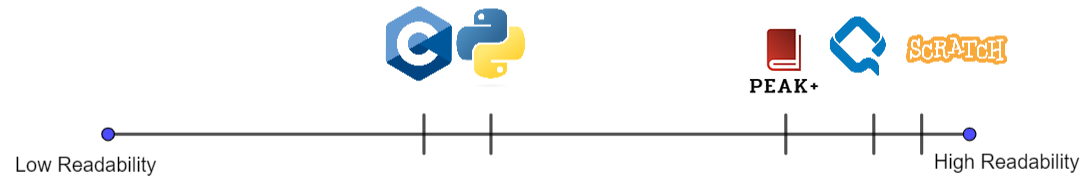
\includegraphics[width=0.9\textwidth]{Files/Billeder: Design/ReadabilityOwn.png}
    \end{center}
    \caption{The programming languages C, Python, Quorum, and Scratch placed on a scale showing readability, including \lang.}
    \label{LD:readability_scale}
\end{figure}


\subsection{Writability}
The writability of \lang is lower since the language should relate to concepts and terminology from high school education. Therefore the language syntax should resemble the English language and math learned in high school. The purpose of \lang is to enable an easy learning curve of the fundamental concepts and implementations used by many of the common industry programming languages.  Furthermore, as \lang is intended to be an introductory language, a focus of the language will not be creating large and optimized applications. \\

That being said, one goal of \lang is to introduce beginner programmers to the use of methods and procedures, which supports a level of abstraction within the language. Because methods are a core principle within programming, they will be implemented, in a manner that supports readability.\\

On the scale displayed in figure \ref{LD:Writability_Scale}, \lang has been placed between C and Quorum, but closer to C. This is due to the fact that the language will have low expressivity, limited support for abstraction (no object-oriented constructs), and a limited amount of data types. Like Quorum, the focus of this language is more on readability in preference to writability. Like Quorum, the goal will be for beginners to be able to quickly recognize and understand the language, and therefore most reserved keywords will not be abbreviations like in many languages.


\begin{figure}[H] 
    \begin{center}
        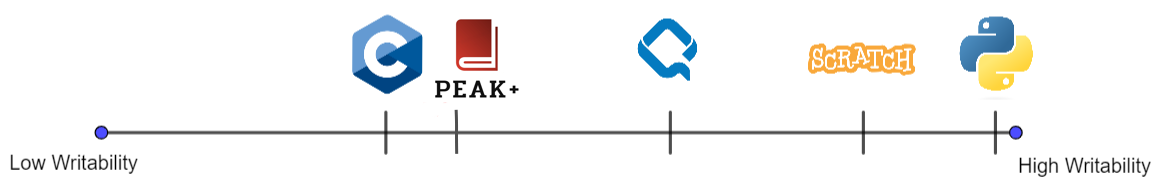
\includegraphics[width=0.9\textwidth]{Files/Billeder: Design/WritabilityOwn.png}
    \end{center}
    \caption{The programming languages C, Python, Quorum, and Scratch placed on a scale showing writability, including \lang.}
    \label{LD:Writability_Scale}
\end{figure}

\subsection{Reliability} \label{LanguageDesign:Realiability}
The importance of reliability is to ensure that the language does what the programmer specifies it to do, within the boundaries of the language. In \lang, there are certain standards that need to be upheld within reliability, in order to cater to a beginner programmer. \\

The language will use static type checking, which should increase the reliability compared to dynamic type checking since the programmer will have to make sure types are appropriately used. On top of this to further simplify the language and improve reliability, aliasing will be restricted by not allowing pointers in the language. From our personal experience, pointers are a tricky programming construct to understand and use, and it is therefore inappropriate to allow aliasing in a language made for beginner programmers. As \lang will have limited or restricted aliasing and no exception handling, it is placed between C and Quorum on the reliability scale in figure \ref{LD:reliability_scale}.

\begin{figure}[H] 
    \begin{center}
        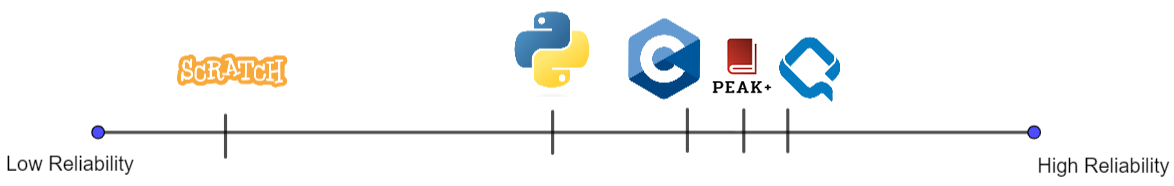
\includegraphics[width=0.9\textwidth]{Files/Billeder: Design/ReliabilityOwn.png}
    \end{center}
    \caption{The programming languages C, Python, Quorum, and Scratch placed on a scale showing reliability, including \lang.}
    \label{LD:reliability_scale}
\end{figure}


\section{The Paradigm of \lang}
Because the goal is to make a beginner-friendly programming language, which aims to make it easier for its users to transition to industry standard languages, the chosen paradigm for \lang is an imperative and procedural paradigm. They have been chosen because, in our own experience, it is important to learn basic programming concepts first like defining basic programming instructions and scopes. An object-oriented approach is deemed too advanced and unnecessary, as we only want to include basic concepts such as functions, control structures, and some basic data types. The same reasons apply to why the functional paradigm has not been chosen. The paradigms mentioned here have been previously explained in section \ref{text-basedlanguages}

\section{Requirements} \label{requirements}
In order to develop a programming language for beginner programmers, requirements must be set. The requirements for \lang are displayed in table \ref{tab:requirements}. 

\begin{table}[H]
\resizebox{\textwidth}{!}{%
\begin{tabular}{|l|ll}
\hline
\textbf{Priority} & \multicolumn{1}{l|}{\textbf{ID}} & \multicolumn{1}{l|}{\textbf{Requirements}} \\ \hline
\multirow{6}{*}{Must Have} & \multicolumn{1}{l|}{M1} & \multicolumn{1}{l|}{\begin{tabular}[c]{@{}l@{}}Declaration and assignment of number, decimal, text, \\ and boolean variables.\end{tabular}} \\ \cline{2-3} 
 & \multicolumn{1}{l|}{M2} & \multicolumn{1}{l|}{Display output and take keyboard input in the console.} \\ \cline{2-3} 
 & \multicolumn{1}{l|}{M3} & \multicolumn{1}{l|}{Basic iterative and selective control structures} \\ \cline{2-3} 
 & \multicolumn{1}{l|}{M4} & \multicolumn{1}{l|}{Basic arithmetic \& logical operations.} \\ \cline{2-3} 
 & \multicolumn{1}{l|}{M5} & \multicolumn{1}{l|}{\begin{tabular}[c]{@{}l@{}}Syntax which resembles concepts and terminology used in \\ high school education.\end{tabular}} \\ \cline{2-3} 
 & \multicolumn{1}{l|}{M6} & \multicolumn{1}{l|}{Error messages at compile time.} \\ \hline
\multirow{4}{*}{Should Have} & \multicolumn{1}{l|}{S1} & \multicolumn{1}{l|}{A foreach loop.} \\ \cline{2-3} 
 & \multicolumn{1}{l|}{S2} & \multicolumn{1}{l|}{String concatenation.} \\ \cline{2-3} 
 & \multicolumn{1}{l|}{S3} & \multicolumn{1}{l|}{Declaration and assignment of lists.} \\ \cline{2-3} 
 & \multicolumn{1}{l|}{S4} & \multicolumn{1}{l|}{List helper functions like add and remove from the list.} \\ \hline
Could Have & \multicolumn{1}{l|}{C1} & \multicolumn{1}{l|}{Support for abstraction in the form of methods} \\ \hline
Won't Have & \multicolumn{1}{l|}{W1} & \multicolumn{1}{l|}{Exception Handling} \\ \hline
\end{tabular}%
}
\caption{MoSCoW requirement table.}
\label{tab:requirements}
\end{table}


The requirements are designed in the light of the target group, beginner programmers. By looking at several different programming tasks given in different beginner programming courses, more features necessary for a beginner language have been settled, leading to the requirements for \lang. The tasks that are examined, are from the imperative programming course in the first semester of our own education\cite{C-CourseExercises}, Python practice exercises from python.org\cite{PythonBasicsExercise} and general code challenges from codecademy.com \cite{CodeAcademyExercises}. Besides examining programming tasks, the requirements are also defined with the language criteria in section \ref{languageCriteriaForLang} in mind.\\

The language has to implement fundamentals for a programming language, including declarations and assignments of variables (M1) and the ability to generate an output to the console and read keyboard inputs (M2). Another fundamental requirement is the use of different types of control structures, both selective and iterative. Examples of beginner tasks include repeating some code $x$ times or as long as a condition is satisfied. In relation to the decision stated in section \ref{Lang Readability} about \lang prioritizing readability, the control structures in \lang have to be concrete and easy for the beginner programmer to understand. In (M3) the definition of basic control structures includes the implementation of if-else condition blocks, a counting loop and a conditional loop. \\ 

To ensure the readability of \lang, the syntax has to resemble concepts and terminology used in high school, e.g. the use of fully spelled words and basic math symbols, leading to requirements M4 and M5. In addition to this, requirement S2 about string concatenation is implemented, as context to compound words. \\

Since \lang is a beginner language, it is important that there are error messages at compile time. This relates to requirement M6.
\\

Different ways of storing related variables are also common in the tasks. For example, saving several variables in a list, deleting an entry in a list, and getting a variable from an entry in the list, leading to requirements S3 and S4. 
\\

Scopes and Functions are also relevant topics. This entails functions which have the possibility of receiving an input and returning an output. This relates to requirement C1. 
\\

\lang will not have exception handling. This feature is deemed as nice to have, but the aforementioned features have been deemed more important due to having a higher impact on the simplicity of \lang.   


\section{Syntax Design} \label{sec:SyntaxDesign}
To create the language specification for \lang, the first step is defining the syntax. Syntax describes the grammar and structure of valid programs in a language. The syntax design is followed up by operational semantics and type rules in section \ref{operational_Semantics}.
This section will cover theoretical sections about context free grammar and Backus-Naur Form, followed up by the context free grammar for \lang.

% Certain precautions should be noted with the decision of having number and decimal. In order to increase simplicity, the first intuition was to only implement one type \textit{number}, encapsulating both integer numbers and decimal numbers. Generalizing all instances of a number into one type would need to be dynamically handled by the compiler. Furthermore, it could lead to less readability in the language control structures, (ref til section), since counting loops should not work with decimals. In order to deal with this issue, all integer numbers will internally be \textit{number} and all decimal numbers have to be \textit{decimal} 


\subsection{Context-Free Grammars} \label{LD: CFG}
A context free grammar (CFG) is a way to formally represent the syntax of a language using symbols and rules. They describe all possible programs that are syntactically correct in the language. A CFG is specified as having a finite set of terminal and non-terminal symbols as well as a start symbol and a finite set of production rules \cite{SPO_Topic_5}. An example of a CFG is displayed in listing \ref{list:CFGExample}.

\begin{lstlisting}[language=scriptkid, label={list:CFGExample},caption=An example of a CFG. The language accepts strings of zero or more A's followed by a 'b' ]
Start -> A B $
A -> A a | epsilon
B -> b
\end{lstlisting}

A terminal symbol is a symbol from the language's alphabet\cite{SPO_Topic_5}. These are always written in lowercase letters. The non-terminal symbols are placeholders for terminal symbols or patterns of terminal symbols. These are written with the first character in uppercase. Non-terminal symbols are derived into other terminals and/or non-terminals until they become exclusively terminal symbols. This is done using production rules \cite{SPO_Topic_5}. Reviewing the CFG in listing \ref{list:CFGExample}, it can consists of several production rules. A production rule describes a possible way, in which a non-terminal can expand. The LHS (left-hand-side) of the arrow in each production rule consists of a non-terminal, that is to be derived. The rules to derive the nonterminal are given by the RHS (right-hand-side). There can be several different ways a non-terminal can be rewritten. The different production rules for a non-terminal are separated by a line '|' and can contain combinations of terminals and non-terminals as well as having the possibility of being epsilon ($\epsilon$), meaning an empty string. Furthermore, the first non-terminal in the LHS of the CFG is the start symbol \cite{SPO_Topic_5}. \\
The terminals in the example in listing \ref{list:CFGExample} are \textit{a}, \textit{b}, and \textit{\$}. The start symbol is 'Start' which can be derived into \textit{A B} followed by the \textit{\$}, end of input stream symbol. The process continues until no non-terminal remains in the derived string. In listing \ref{list:CFGExample}, \textit{A} is either derived to epsilon at the beginning or recursively derived into \textit{A a} until the nonterminal \textit{A} derives into epsilon. Furthermore, \textit{b} is derived from the nonterminal \textit{B}. \\

A CFG can be represented using BNF (Backus-Naur Form) or EBNF (Extended Backus-Naur Form). The set of strings that a CFG can define is called its language. A string that belongs to the language of the CFG, can be considered a valid string for the CFG \cite{SPO_Topic_5}. The notation of a CFG can vary, but in this report, productions for non-terminals are shown using an arrow '->'.

\subsection{Backus-Naur Form}
BNF (Backus-Naur Form) and EBNF (Extended Backus-Naur Form) are two ways to represent a CFG\cite{SPO_Topic_5}. In \lang, BNF has been used to represent the CFG. An advantage of using BNF over EBNF is that BNF is simpler in the way that it only uses a small set of metacharacters\cite{IBM} and rules which are easy to learn and understand. A disadvantage of using BNF instead of EBNF is that BNF uses a larger amount of productions to describe the same grammar as EBNF. This can make the grammar more difficult to read than EBNF which can especially be a problem when creating complex grammar.\\ 
EBNF extends BNF by using elements similar to regular expressions, such as "[]" to indicate an optional element or "\{\}" to indicate repetition zero or more times\cite{SPO_Topic_5}.\\
Overall, the advantages of using BNF are that it is simpler to learn and understand, as it has fewer metacharacters. Furthermore, most CFG tools do not recognize EBNF. For these reasons, we will write the CFG of \lang using BNF.

\subsection{Context-Free Grammar for \lang} \label{CFGForLang}
The \lang programming language focuses on being simple in its syntax and data structures, while also implementing common principles from the programming industry for an easier transition from a beginner language to a language such as C or C\#.\\

In order to make the language easier to understand for new programmers, only 5 data types will be implemented. Three of these data types are primitive, being \textit{number}, \textit{decimal} \& \textit{boolean}. The other two are non-primitive data types being \textit{text} \& \textit{list}. The data type \textit{number} is an integer, and \textit{decimal} is a floating point number. To increase readability, the \textit{boolean} is a boolean value, having either the value \textit{true} or \textit{false}. Conditional operators taught in high school mathematics are included, such as '\textit{<}' and '\textit{<=}'. The logical \textit{or} and the logical \textit{and} are written in text as these operators are not introduced in the high school curriculum. \textit{text} is a string, which is a collection of characters, and \textit{list} is a collection of any of the previous types. \\
% and a feature that is aimed to be implemented is string concatenation via the "+" operator. This allows for better readability of strings. 

%Any instance of the \textit{text} variable will be seen by the compiler as a collection of chars. In regards to string manipulation. Another feature that is aimed to be implemented is string concatenation via the "+" operator. This allows for better readability of strings. \lang will also implement \textit{Lists} as a type, which aims to generalize any collection of a single type into one data type. \\ This highlights simplicity and orthogonality within \lang. 

\textbf{Overall program structure:} The overall structure of the \lang programming language can be seen in listing \ref{list:CFGOverallStructure}. A program in \lang consists of a list of commands, which can be further broken down into either a statement or a declaration. A declaration consists of a type, an id, and an optional assignment, whereas a statement can be broken further into multiple different productions. Like in many other languages, a semicolon ';' is used as a statement terminator, making it clear when a statement ends. Using semicolons as a statement terminator instead of, for example, a newline, also allows the programmer to span a long statement across multiple lines, making it more readable. This makes it so anyone reading the code is able to read a long statement without having to scroll left and right in their editor. It also allows for multiple statements on a single line.\\

\begin{lstlisting}[language=scriptkid, label={list:CFGOverallStructure},caption=Overall structure of \lang CFG]
Program        -> Cmds 
Cmds           -> Cmd Cmds | EPSILON 
Cmd            -> Stmt | Dcl 
Dcl            -> Type Id Ass ; 
Ass            -> = Expr | EPSILON 
Stmt           -> Id = Expr ; | CtrlStrct | ListStmt ; | FuncDef | FuncCall ;
\end{lstlisting}

\noindent\textbf{Control structures: } The control structures of \lang can be seen in listing \ref{list:CFGCtrlStrct}. A control structure in \lang can be either a selective control structure (if statement), or an iterative control structure (loop). This can be seen from the Non-terminal \textit{CtrlStrct} in listing \ref{list:CFGCtrlStrct}, which can derive from the productions \textit{IfStmt} or \textit{Loop}. \\ 
When deciding on control structures, the standard if-else blocks are used to support readability. However, in regards to loops, it has been decided to generalize all loops by using the reserved word \textit{repeat}, instead of the standard \textit{for} and \textit{while}. This is based on the analysis of the Quorum programming language, which simplifies the standard loop structures. 
\\

\begin{lstlisting}[language=scriptkid, label={list:CFGCtrlStrct},caption=Control structure of \lang CFG]
CtrlStrct -> IfStmt | Loop   
IfStmt -> if ( Expr ) Block ElseIfStmt   
ElseIfStmt -> else if ( Expr ) Block ElseIfStmt | Else | EPSILON   
Else -> else Block   
Loop -> repeat Loops   
Loops -> LoopStmt | WhileStmt | ForeachStmt   
LoopStmt -> ( Expr ) times Block 
WhileStmt -> while ( Expr ) Block   
ForeachStmt -> for each ( Type Id in Id ) Block   

\end{lstlisting}

\noindent \textbf{If statement: } An if statement in \lang starts with the terminal keyword \textit{if}, followed by an \textit{Expr} nonterminal encapsulated by parentheses, a \textit{Block} and an optional \textit{ElseIfStmt} (See line 2 in listing \ref{list:CFGCtrlStrct}). An \textit{ElseIfStmt} production has the same structure as an \textit{IfStmt}, but with the terminals \textit{else if} instead of just \textit{if}. Furthermore, it derives to the nonterminal \textit{Else} and \textit{EPSILON}, making the \textit{ElseIfStmt} optional as it has a production that derives to nothing. An advantage of this structure is that it allows for checking multiple expressions and even nesting if statements, which makes writing complex conditional logic easier. However, this can also turn into a disadvantage, as deeply nested code may confuse the programmer as it will be harder to read and understand.\\

%An advantage of this structure having a \textit{Block} in an if statement, and a block being able to derive back to an if statement, is that it allows for nested conditional statements. Howe\\\

\textbf{Loops: } A loop in \lang will always derive to the \textit{repeat Loops} production as can be seen on line 5 in listing \ref{list:CFGCtrlStrct}. This means that any loop will consist of the terminal keyword \textit{repeat}, followed by one of the different loop types defined in listing \ref{list:CFGCtrlStrct}. Having the structure consist of the terminal \textit{repeat} followed by a loop type, provides a consistent way to define and identify loops in \lang. A disadvantage of this is that it adds an extra word to the language every time a loop is created, which gives the language slightly less writability. However, as previously mentioned in section \ref{Lang Readability}, readability is prioritized above writability in \lang.\\

\lang has three kinds of loops being a counting loop, a while loop, and a for each loop. The counting loop has the following syntax: "repeat (x) times{}". This is a simple loop, which is intended for beginners to get familiar with loops in their simple form. The loop requires an integer number or variable of the type \textit{number} to determine how many times the loop should run. The while loop functions as in any other programming language, where it runs as long as a condition is fulfilled. The while loop is deemed necessary for the language, as it is able to achieve more than other loop constructs. Finally, the \textit{for each} loop has been selected for the \lang language in order to provide a simple way of looping through each element in a collection. This is simpler than a normal \textit{for} loop as a \textit{for each} loop only requires an initializer expression and the collection to loop through. In comparison, a for loop requires both an initializer expression(s), a continue expression, and an update expression(s). A for-loop syntax may be difficult for beginner programmers to remember, so, therefore, a for-loop control structure will not be included in the language. \\

\textbf{Functions: } The function definition of \lang can be seen in listing \ref{list:CFGCtrlStrct}. A function definition in \lang starts with the terminal \textit{function} followed by an \textit{Id}, a list of parameters, the function return type, and finally the function body. 

\begin{lstlisting}[language=scriptkid, label={list:CFGFunction},caption=Function call \& declaration of \lang CFG]
FuncCall -> call Id ( ArgList ) | call output ( ArgList ) | call Type input ( ArgList ) 
FuncDef -> function Id ( ParamList ) FuncReturn Block   
FuncReturn -> return FuncReturnType   
FuncReturnType -> Type | nothing   
ParamList -> Param ParamTail | EPSILON   
ParamTail -> , Param ParamTail | EPSILON   
Param -> Type Id   
ArgList -> Expr ArgTail | EPSILON   
ArgTail -> , Expr ArgTail | EPSILON   

\end{lstlisting}

The \textit{function} terminal is used in order to clearly define that a function is being defined, increasing readability. The return type is placed after the parameter list. This choice is made in order to obtain readability by separating the return type from the start of the declaration. Explicitly having to use the return keyword along with the function keyword in a function definition provides less writability, but more readability. 
The \textit{FuncReturnType} nonterminal derives to either a \textit{Type}, or \textit{nothing}. The \textit{nothing} return type is equivalent to the void return type in other languages. The \textit{nothing} keyword is used instead, due to the fact that returning \textit{nothing} seems more intuitive than \textit{void} for beginner programmers. 

The \textit{FuncCall} nonterminal has one production, starting with the terminal \textit{call}, followed by an \textit{Id} and an \textit{ArgList} enclosed by parentheses. The \textit{call} keyword is used to once again increase readability, as it helps clearly define when a function is called. \\

\textbf{Input \& output: } The definition of input and output for \lang can be seen in listing \ref{list:CFGInputoutput}. The \textit{output} terminal is used as a way to write / print something to the console. Whereas the \textit{input} terminal is a way to read input from the user. 
\begin{lstlisting}[language=scriptkid, label={list:CFGInputoutput},caption=Input \& output of \lang CFG]
FuncCall -> call Id ( ArgList ) | call output ( ArgList ) | call Type input ( ArgList )
.
.
.
ArgList -> Expr ArgTail | EPSILON   
ArgTail -> , Expr ArgTail | EPSILON 
\end{lstlisting}
The input and output definition starts with the non-terminal \textit{FuncCall} which can derive to either \textit{call output} or the \textit{call Type input}. As can be seen in listing \ref{list:CFGInputoutput}, both the terminal \textit{input} and the terminal \textit{output} takes the non-terminal \textit{ArgList} as a parameter. The non-terminal \textit{ArgList} derives into an expression followed by the next non-terminal \textit{ArgTail}. In the CFG, the input may contain multiple expressions. However, in the compiler, the \textit{ArgList} for the input function should only be able to contain a single expression, being a variable of the type defined after the \textit{call} terminal. The reason for using \textit{ArgTail} instead of \textit{Id} in the input even though the input is essentially an id, is to keep consistency among functions, following the general function definition structure. 
\\

\textbf{Lists:} A list in \lang starts from the non-terminal \textit{Stmt} which then derives to the non-terminal \textit{ListStmt} production as can be seen in listing \ref{list:CFGList}.
\begin{lstlisting}[language=scriptkid, label={list:CFGList},caption=Lists in \lang CFG]
Program -> Cmds   
Cmds -> Cmd Cmds | EPSILON   
Dcl   
Dcl -> Type Id Ass ;   
Ass -> = Expr | EPSILON   
Stmt -> Id = Expr ; | CtrlStrct | ListStmt ; | FuncDef | FuncCall ; | CommentStmt ; | return Type ; 
.
.
.
ListStmt -> ListOpr | ListOprExpr 
ListOpr -> Id : Add ( ArgList ) | Id : Replace ( ArgList ) 
ListOprExpr -> Id : IndexOf ( Expr ) | Id : ValueOf ( ArgList ) 
\end{lstlisting}
The non-terminal \textit{ListStmt} can derive either the non-terminal \textit{ListOpr} or the non-terminal \textit{ListOprExpr}. A \textit{ListStmt} will always start with the terminal \textit{Id}, which refers to the Id of the list being operated on. If going from the non-terminal \textit{ListOpr} it is possible to derive to the terminal \textit{Add}, to add an element to the list, or derive to the terminal \textit{Replace} in order to replace an element in the list.\\
The non-terminal \textit{ListStmt} can also derive from the non-terminal \textit{ListOprExpr}. The \textit{ListOprExpr} can derive into the terminal \textit{IndexOf} to get the index of a position in the list, or the terminal \textit{ValueOf} to get the value stored in a specific position in the list.


\subsection{Operator Precedence} \label{OrderPrec}
Operator precedence defines the order in which operators are evaluated in an expression. The operator precedence for \lang follows the basic mathematics rules, this can be seen in table \ref{tab:OperatorPrecedence}. The highest precedence in \lang follows the mathematical PEMDAS operators which are: parenthesis, exponent, multiplication, division, addition \& subtraction\cite{mathnasium}. The exponent operator is not included in the language, as it is achievable through multiplication, and therefore is not strictly necessary. Following the PEMDAS operators come the relational operators, such as "\textit{greater than}" and Logical operators such as "\textit{and}". These have the lowest precedence in \lang. This is because the logical operators are typically used in conjunction with operators with higher precedence to combine or negate a result.


\begin{table}[H]
\centering
\begin{tabular}{|l|l|l|}
\hline
\multicolumn{1}{|c|}{Precedence} & Operator & Description \\ \hline
1 & (  ) & Parenthesis \\ \hline
2 & \begin{tabular}[c]{@{}l@{}}x * y\\ x / y\end{tabular} & \begin{tabular}[c]{@{}l@{}}Multiplication\\ Division\end{tabular} \\ \hline
3 & \begin{tabular}[c]{@{}l@{}}x + y\\ x - y\end{tabular} & \begin{tabular}[c]{@{}l@{}}Addition\\ Subtraction\end{tabular} \\ \hline
4 & \begin{tabular}[c]{@{}l@{}}x \textgreater  y\\ x \textgreater{}= y\\ x \textless y\\ x \textless{}= y\end{tabular} & \begin{tabular}[c]{@{}l@{}}Greater than\\ Greater than or equal to\\ Less than\\ Less than or equal to\end{tabular} \\ \hline
5 & \begin{tabular}[c]{@{}l@{}}x is y\\ x is not y\end{tabular} & \begin{tabular}[c]{@{}l@{}}Is equal to\\ Is not equal to\end{tabular} \\ \hline
6 & x and y & Logical and operator \\ \hline
7 & x or y & Logical or operator \\ \hline
\end{tabular}
\caption{Operator Precedence for \lang}
\label{tab:OperatorPrecedence}
\end{table}

\subsection{Scope Rules} \label{sec:scope_rules}
Scope rules regulate the visibility of identifiers in a programming language. They relate every applied occurrence of an identifier to a binding occurrence. The binding occurrence is defined as the instance where an identifier is declared initially, and the applied occurrence is any point at which the identifier is used as part of an expression \cite{craftingcompiler}. Both of these occurrences can be seen in listing \ref{list:binding}. Different scope rules give rise to different interpretations of the same piece of code \cite{transtrees}. 

\begin{lstlisting}[language = scriptkid, label={list:binding},caption=Example of a binding occurence and an applied occurence of the identifier \textit{x} in \lang]
number x = 1; // Binding Occurence

number r = x + 1; // Applied Occurence
\end{lstlisting}

\noindent
There are two kinds of scope rules: Dynamic and static. Dynamic scope rules employ the bindings known when the procedure is called and are based on the program's runtime. Static scope rules employ the bindings known when the procedure is declared and are based on the structure of the program\cite{transtrees}. \lang will use static scope rules. The main reason for this choice is to strengthen the readability of \lang. \lang uses the nested block structure. A nested block structure means, that a program can be subdivided into several disjoint blocks with an infinite amount of blocks inside each block. A block is an area of text in the program that corresponds to some kind of boundary for the visibility of identifiers. The essence is that several local definitions of a single identifier may occur in different blocks (but not in the same block) \cite{craftingcompiler}.
The reason for this is to enable flexibility for the beginner programmer. A nested block structure is also a common industry standard, which prepares the programmer for those languages. The scope rules for \lang are:

\begin{itemize}
  \item A \textit{block} in \lang can be a \textit{function} or control structure, like \textit{if}-statements. \lang also contains special characters like \textit{repeat} and \textit{repeat for each} that iterate over a block a defined amount of times.
  \item All blocks are defined by using the prefix for one of the above and encapsulating the content between two curly brackets, this can be seen in listing \ref{list:block}.
  \item A local variable declared inside a block can only be applied within that block and any nested blocks within it. Variables declared globally can be used anywhere.
  \item Variable shadowing is allowed within nested blocks.
  \item  
  Functions have to be declared in the global scope, and cannot be redeclared in any scope. 
\end{itemize}

\begin{lstlisting}[language=scriptkid, label={list:block},caption=Example of a Block]
function Sum(number x, number y) return number 
{ 
    return = x + y; 
} 
\end{lstlisting}

\newpage
\section{Semantics}
To settle the behavior of the language, the next step in the language specification for \lang is defining the semantics. This section covers abstract syntax, type rules, and operational semantics. The subsections will be structured with theoretical knowledge, followed up by the constructs from \lang. \\

The source of the knowledge described in this section is from the course Syntax and Semantics and will be cited in the paragraph when appropriate. Definitions that are directly from the course material, will also have standard citations, without quotation marks.

\subsection{Abstract Syntax} \label{AST}
%Within most compilers, there exists a phase in which the parse tree derived from the program, is transformed into an abstract syntax tree (AST). The AST simplifies the program, making it easier to handle when further decorating the tree and eventually in the code generation phase. This is further explained in \ref{ASTDesign}.\\

Abstract syntax defines the structure of valid programs in the language but in a more abstract and simplified form. It is for example not concerned with parsing and ambiguity problems and it does not have to comply with the standard formats for parsing algorithms\cite{SS_lecture_8}. The abstract syntax is defined from a combination of a set of syntactic categories, which are seen in table \ref{tab:SyntacticCategories}. A set of formation rules is defined for these syntactic categories, which can be seen in table \ref{tab:formationrules} \cite{SS_lecture_8}. \\

\begin{table}[H]
\begin{tabular}{llll}
\textit{n}   & 	\in & \textbf{Num}     & Natural Numbers       \\
\textit{d}   & \in  & \textbf{Dec}     & Rational Numbers      \\
\textit{txt} & 	\in & \textbf{Text}    & Strings               \\
$\mathbb{T, F}$  & \in & \textbf{Bool}   & Boolean values        \\
\textit{x}   & 	\in & \textbf{Var}     & Variable names        \\
\textit{L}   &  \in & \textbf{List}    & Lists                  \\
\textit{f}   & 	\in & \textbf{Func}    & Function names        \\
\textit{B}   & 	\in & \textbf{BTypes}  & Base Types            \\
\textit{T}   & \in & \textbf{Types}      & All Types             \\
\textit{e}   & 	\in & \textbf{Exp}     & Expressions           \\
\textit{S}   & 	\in & \textbf{Stm}     & Statements            \\
$D_V$           & \in & \textbf{DecVar}  & Variable declarations \\
$D_F$           & \in & \textbf{DecFunc} & Function declarations
\end{tabular}
\caption{Syntactic categories of \lang}
\label{tab:SyntacticCategories}
\end{table}

\noindent The syntactic categories in table \ref{tab:SyntacticCategories} represent all elements in \lang. To represent an element of the syntactic categories we use meta-variables, which are the characters in the first column in the table. E.g the syntactic category \textbf{Num} in the first row, represents any natural number in \lang and the meta variable \textit{n} is used in the abstract syntax to represent an arbitrary number. Lists are defined using $L$ and contain any amount of expressions in an ordered format.\\ 

%Besides numbers, the goal is to implement a decimal value as well, in order to handle certain divsions and general arithmetic's with decimal numbers. The problem with generalizing every \textbf{Num} instance into a floating point number, is that non-integer numbers are generally not compatible with indexing lists.The \textbf{Text} variables are handled as a sequence of characters. \textbf{Lists} are stored in the heap, in order to dynamically declare them, the reason for this is to increase flexibility of the language, in order to cater towards beginner programmers. 

\begin{table}[H]
\resizebox{\columnwidth}{!}{%
\begin{tabular}{lll}
\textit{B}  & ::= & number | decimal | text | boolean  \\ \\
\textit{T}  & ::= & \textit{B} | list(\textit{B}) \\ \\
\textit{e}  & ::= &
  \begin{tabular}[c]{@{}l@{}} 
  $n$ | $txt$ | $\mathbb{T}$ | $\mathbb{F}$ | $d$ | $x$ | $e_1$ + $e_2$ | $e_1$ - $e_2$ | $e_1$ * $e_2$ | $e_1$ / $e_2$ | $e_1$ is $e_2$ | $e_1$ is not $e_2$ |\\ $e_1$ > $e_2$ | $e_1$ >= $e_2$ | $e_1$ < $e_2$ | $e_1$ <= $e_2$ | $e_1$ and $e_2$ | $e_1$ or $e_2$ | ($e_1$) | $x$:valueOf($n$) | $x$:indexOf($e$)
  \end{tabular} \\ \\
\textit{S} &
  ::= &
  \begin{tabular}[c]{@{}l@{}} $S_1$ ; $S_2$ | $D_V$ | $D_F$ | $x$ = $e$ | $x$:add($e_1$ , ... , $e_k$) | $x$:insert($e$ , $n$) | \\ if($e$) \{ $S$ \} | If($e$) \{ $S_1$ \} Else \{ $S_2$ \} | repeat ($n$) times \{ $S$ \} | repeat while ($e$) \{ $S$ \} | \\ repeat for each ($B$ $x$ in $x$) | call $f$($e_1$, ... , $e_k$) | x = call $f$($e_1$, ... , $e_k$) | $\epsilon$\end{tabular}\\ \\
$D_V$ & ::= & $T x = e$ ; $S$ | $T x$ ; S | $\epsilon$                   \\ \\
$D_F$ & ::= & function $f$($T_1\ x_1$ , ... , $T_k\ x_k$) return $T$ \{ S_1 ; \ $return$ \ e \} ; \ S_2\ |\ $\epsilon$ \\ \\
\end{tabular}%
}
\caption{Abstract Syntax formation rules}
\label{tab:formationrules}
\end{table}

\noindent The formation rules define the structure of the syntactic categories and are written in the same format as production rules in BNF, explained in section \ref{LD: CFG} \cite{SS_lecture_8}. In the first column in table \ref{tab:formationrules}, it is denoted that an expression \textit{e} in \lang can be one of the related right-hand side formation rules. \\

The syntactic categories \textbf{Num}, \textbf{Dec}, \textbf{Text}, \textbf{Bool}, \textbf{Var} and \textbf{Func} do not have formation rules as they are trivial. For example, \textbf{Text} is a string of characters, as explained in section \ref{LD: CFG}. 

\subsection{Type Rules} \label{sec:TypeRules}
To prevent a program to execute with errors, a type system is important. When compiling a program, the type systems' purpose is to catch type errors before the program executes. When a program executes without type errors it is called \textit{well-typed}. To know when a program is well-typed, we define type rules. The type rules of a language define how the different types in the language are allowed to be used correctly. \\

%Henceforth, type checking will be done at compile time. Additionally, \lang will use dynamic binding, meaning all variable declarations can be reassigned, and re-declared within a nested scope. Functions can be declared once within a specific scope. 

In the type system, values of variables are kept in an environment. As variables get declared or reassigned, they are updated in the environment \cite{SS_lecture_10}. A type environment keeps track of the types of variables. A type environment is a partial function that maps variables to types, \textit{E} : \textbf{Var} $\cup$ \textbf{Func} $\rightharpoonup$ \textbf{Types} \cite{SS_lecture_10}. When the state is changed in the environment it can be denoted as $E[x \mapsto T]$. The formal definition of an update to the environment is the following function:

\begin{equation}
    (E[x\mapsto T])(y) = \begin{cases}E(y) &  y \neq x\\T & y = x\end{cases}
\end{equation}

\noindent To define a type system, the first step is to describe a collection of formal statements called \textit{judgments} \cite{SS_lecture_10}. The two types of judgments that are used in the type system, are seen in definition \ref{judgments}\cite{SS_lecture_10}. 
\begin{equation} \label{judgments}
    \begin{split}
        E \vdash e:T \\ E \vdash S:ok
    \end{split}
\end{equation}

\noindent
In definition \ref{judgments} it can be read as, within the environment \textit{E} some assertion of a syntactic category is made. In the first judgment, we assert that an expression \textit{e} has a certain type, and in the second judgment, we assert that a statement \textit{S} is well-formed in accordance with the formation rules. The judgment will be derived from the type rules defined in the type system. Such derivations can be used to describe this system. Definition \ref{derivation_example} is the template for how the derivations will be presented\cite{SS_lecture_10}.

\begin{equation} \label{derivation_example}
    \frac{E_1 \vdash \alpha_1 , ..., E_n \vdash \alpha_n}{E \vdash \alpha}
\end{equation} 

\noindent The $\alpha$ represents a syntactic category implementation and can be any of the two mentioned judgments in definition \ref{judgments}. Based on the explained rules, the type system of \lang can be formally described. \\

The standard derivation for a variable can be performed when a variable reaches its final possible derivation. In definition \ref{Varts} the derivation checks if a variable's type matches what is in the environment.

\begin{equation} \label{Varts}
    (VAR_{TS})\frac{E(x) \ = \ T}{E \ \vdash x \ : \ T}
\end{equation} \\

\noindent As mentioned in section \ref{sec:scope_rules}, \lang allows 
variable shadowing, meaning a variable can be redeclared in an inner scope. Furthermore, type errors can occur when expressions are made with types that are not compatible. 
Firstly, the type rules for expressions can be seen in definitions \ref{expression_rules}, \ref{Dec*_ts}, \ref{TXTts}, and \ref{Bool*_ts}.

\begin{equation} \label{expression_rules}
  (NUM*_{TS})\frac{E \ \vdash \ e_1 : \ number \ E \ \vdash \ e_2 : \ number \ }{E \ \vdash e_1 \star \ e_2 \ : \ number} \ \ \ \
  where \ \star \in \{ +, *, - \}  
\end{equation}
    
\begin{equation} \label{Dec*_ts}
    (DEC*_{TS})\frac{E \ \vdash \ e_1 : \ decimal \ E \ \vdash \ e_2 : \ decimal \ }{E \ \vdash e_1 \star \ e_2 \ : \ decimal} \ \ \ \
    where \ \star \in \{ +, *, - , /\},\ and\ e_2 \neq 0
\end{equation}
    
\begin{equation} \label{TXTts}
        (TXT_{TS})\frac{E \ \vdash \ e_1 : \ text \ E \ \vdash \ e_2 : \ text \ }{E \ \vdash e_1 + \ e_2 \ : \ text} 
\end{equation}

\begin{equation} \label{Bool*_ts}
    (BOOL*_{TS})\frac{E \ \vdash \ e_1 : \ number \ E \ \vdash \ e_2 : \ number \ }{E \ \vdash e_1 \star \ e_2 \ : \ boolean} \ \ \ \
    where \ \star \in \{ >, <, \geq, \leq, is, is \ not \}
\end{equation}

\noindent Addition can occur both in an arithmetic sense between \textbf{Num} and \textbf{Dec}, and in the form of string concatenation. However, string concatenation can only occur between two \textbf{Text} variables.  \textbf{Num} \& \textbf{Dec} is mainly split up to avoid conflicts when using a floating-point value as a list index. In definition \ref{expression_rules} the star cannot be a division symbol. If two numbers are divided, the type will convert to a decimal. It is also not allowed to divide by zero. The rest of the type rules for expressions in \lang are found in appendix \ref{Appendix:TypeSystem} \\

The next syntactic category to define type rules for is variable declarations (meta variable $D_V$ in table \ref{tab:formationrules}). These formation rules allow the declaration and assignment of variables with type \textbf{T}. The derivations in definitions \ref{TYPERULE:Dcl} and \ref{TYPERULE:Ass}, describe the type rules. In $(DEC_{TS})$ the $x \ \notin \ dom(E)$ defines that the variable $x$ is not previously in the domain of the environment $E$. This is necessary because a variable declaration creates an instance of a new variable, and there cannot be any existing variables with the same name in the same scope. 

\begin{equation} \label{TYPERULE:Dcl}
    (DEC_{TS})\frac{x \ \notin dom(E) \ \ E \ \vdash \ e : \ T }{E \ \vdash T \ x \ = \ e  \ : \ ok}
\end{equation}

\begin{equation}\label{TYPERULE:Ass}
    (ASS_{TS})\frac{E(x) = T \ \ E \ \vdash \ e : \ T \ }{E \ \vdash x \ = \ e \ : \ ok}
\end{equation}

\noindent The formation rule of $\epsilon$ is shown in definition \ref{epsilonTS}, since it can appear in multiple formation rules. $\epsilon$ simply derives to a well-formed derivation.

\begin{equation} \label{epsilonTS}
    (EMPTYSTM_{TS})\frac{}{\ E \ \vdash \epsilon \ : \ ok}
\end{equation}

\noindent
The last syntactic category which will be shown here is the function declaration. In definition \ref{funcDec1_TS} the function has a return type T. A function declaration is well-formed when the functions block and return value is well-formed in the environment where the variables $x_1,..,x_k$ have the type $T_1,..T_k$. Furthermore, the statement $S_2$ which is executed after the function call is well-formed in the updated environment. \\

Definition \ref{funcDec2_TS} is almost identical to definition \ref{funcDec1_TS}. The change here is, that for a function without a return type, we do not handle the return type in the premises. \\

\begin{equation} \label{funcDec1_TS}
% Type rules for function declaration
(FUNCDEC1_{TS})\frac{\begin{array}{c}
\\ E' \ \vdash \ S_1 : \ ok \ \ \ E' \ \vdash \ e\ : \ T \ \\
E[f \ \mapsto \ 
(x_1 \ : \ T_1 \ , ... , \ x_k \ : 
\ T_k \  \rightarrow \ T)] \ \vdash S_2 \ : \ ok\end{array}  }
{E \ \vdash function \ f(T_1\ x_1 , ... , T_k\ x_k) 
\ return \ T \ \{ \ S_1; \ return \ e \ \}\ ; \ S_2 \ : \ ok}
\end{equation}
\begin{center}
    $where\ E' =\ E[x_1 \ : \ T_1 \ , ... , \ x_k \ : 
\ T_k ]$ 
\end{center}

\begin{equation} \label{funcDec2_TS}
 % Type rules for function call
(FUNCDEC2_{TS})\frac{\begin{array}{c} E[x_1 \ : \ T_1 \ , ... , \ x_k \ : \ T_k \ ] \ \vdash \ S_1 : \ ok \ \\
E[f \ \mapsto \ 
(x_1 \ : \ T_1 \ , ... , \ x_k \ : 
\ T_k \ )] \ \vdash S_2 \ : \ ok\end{array}  }
{E \ \vdash function \ f(T_1\ x_1 , ... , T_k\ x_k) 
\ return \ nothing \ \{ S_1 ; \ return \}\ ;\ S_2 \ : \ ok}
\end{equation}

\noindent There are two ways to handle a function call. As displayed in the formation rules in table \ref{tab:formationrules}, it can either be $call \ f()$ or $x = call \ f()$. In definition \ref{funcCall1_TS}, the left-most derivation checks if there exists a function with the name $f$ which associates to the formal parameters and return type listed. Thereafter each argument given is crosschecked with the appropriate type to make sure they match. If so the derivation is successful. In definition \ref{funcCall2_TS} one more premise is added to the derivation, where we check that the variable $x$ in the environment has type $T$. The rest of the type system can be found in Appendix \ref{Appendix:TypeSystem}.

\begin{equation} \label{funcCall1_TS}
      (FUNCCALL1_{TS})\frac{E(f)\ =\ (x_1: T_1 ,...x_k\ :\ T_k\ \rightarrow\ T) \ \ E \ \vdash \ e_i \ : \ T_i \ }
{E \ \vdash call \ f(e_1,...,e_k) \ : \ ok} \ \ where \ i = 1...k
\end{equation}

\begin{equation}\label{funcCall2_TS}
     (FUNCCALL2_{TS})\frac{E(f)\ =\ (x_1: T_1 ,..., x_k : T_k\ \rightarrow\ T) \ \ E(x)\ = \  T \ \ \ E \ \vdash \ e_i \ : \ T_i \\ }{E \ \vdash x \ = \ call\ f(e_1,...,e_k) \ : \ ok} \ \ where \ i = 1...k
\end{equation}

\subsection{Operational Semantics} \label{operational_Semantics}
Before, the structural operational semantics for \lang can be defined, there is some theory that needs to be explained. Firstly, several forms of semantics exist. Semantics that this report will not cover includes denotational semantics, which focuses on the effect of executing programs by assigning a denotation to them, and axiomatic semantics, which focus on the correctness property of programs \cite{SS_lecture_8}. The semantics that are important to look at in this context are operational semantics. Operational semantics are descriptions of the meaning of a program, precisely telling you how it should execute. To define the operational semantics, we use Transition Systems.

\subsubsection{Transition Systems}
A Transition System is a directed graph and can be defined as a 3-tuple. The formal definition can be seen in definition \ref{transitionSystemTuple} \cite{SS_lecture_8}. 

\begin{equation} \label{transitionSystemTuple}
    S = (\Gamma, \rightarrow, T)
\end{equation}

\noindent The first symbol ($\Gamma$) represents the set of configurations. Each configuration is a vertex of the graph and they represent the current state of the program. An example of this is to think of each vertex containing the known variables which have been declared at that point throughout execution. The arrow symbol ($\rightarrow$) is the transition relation, formally written $\rightarrow \subseteq (\Gamma \backslash T) \times \Gamma$.
%which can be read as a subset of the cross-product between all configurations not including the terminal configurations, to all configurations 
Transitions are the edges of the graph, which act as a bridge between the configurations. From each configuration, you can take the possible transitions to get to another configuration. Each transition is written as a pair ($a$, $b$) where $a$ can transition to $b$. The last symbol ($T$) is the set of terminal configurations. A terminal configuration is a configuration that you cannot transition away from and it is a subset of $\Gamma$, written $T \subseteq \Gamma$. \cite{SS_lecture_8} \\

We took a structural approach to the operational semantics a.k.a (SOS) because it allows us to define the operational semantics based on a few rules. Having SOS means that the transition system has to comply with the following three rules.

\begin{itemize}
    \item Determine the format of the transition (all transitions must comply with the chosen format)\cite{SS_lecture_8}. 
    \item The configurations that are the source of a transition should be terms generated from the abstract syntax in table \ref{tab:formationrules} \cite{SS_lecture_8}.
    \item Define the transition relation by means of structural                 derivation rules\cite{SS_lecture_8}.
\end{itemize} \\

\noindent The format for each syntactical group will be defined later in subsection \ref{TSytstem:Lang} where the transition system for \lang is explained.

%Now that the general concept of the transition system is defined, we can use it to set some \textit{derivation rules} which are "rules that define how the program state changes based on the language construct in focus" \cite{STEP}. The derivation rules will be explained in the following sections using the Big-Step Semantics. 


\subsubsection{Big-Step and Small-Step Semantics} \label{big-step_Chapter}
When deciding to define the operational semantics for a language, two methods can be used. \textbf{Big-Step} semantics and \textbf{Small-Step} semantics. Both of these semantic types can be expressed as the transition system defined in definition \ref{transitionSystemTuple}.

\begin{itemize}
    \item \textbf{Big-Step} semantics (BS) express an entire computation of a given configuration's transition ($\gamma \in \Gamma$) to its terminal configuration ($t \in T$) \cite{SS_lecture_8}. 
    \item "\textbf{Small-Step} semantics (SS) express each transition as a
    single step of a larger computation. Terminal configurations
    characterize when the computation stops" \cite{SS_lecture_8}.
\end{itemize}

\noindent
Small-step semantics are often used when more detail about a derivation is required to understand what is happening. Often it is used in concurrency, where multiple executions in a program are happening at the same time\cite{SS_lecture_12}. For the sake of simplicity as well as the fact that \lang does not have concurrency capabilities, the semantics will be described using Big-Step semantics. \\

To show the basic concept of Big-step semantics, an example of the arithmetic summation of two numbers is shown in definition \ref{bigStep-example}. Here the format of the transition is $a \ \rightarrow _{\textbf{Exp}} v$ where $a \in \textbf{Exp}$ and $v \in \mathbb{Z}$. The transition symbol $\rightarrow _{\textbf{Exp}}$ can be read as "evaluates to an instance of the expression category" \cite{SS_lecture_8}.

\begin{equation} \label{bigStep-example}
    (PLUS_{BS})\frac{a_1 \ \rightarrow _{\textbf{Exp}} \ v_1 \ \ a_2 \ \rightarrow _{\textbf{Exp}} \ v_2}
    {a_1  +  a_2 \rightarrow _{\textbf{Exp}} \ v_1  +  v_2}
\end{equation}

\subsubsection{Environment-Store Model}
Choosing to write the semantics of a programming language in the format shown in definition \ref{bigStep-example} is not extensive enough for \lang. It is unable to handle the scope rules set out for \lang in section \ref{sec:scope_rules} since it assumes a monolithic-block structure. To handle this we use a concept known as the \textit{Environment-Store Model}. This model acts as an addition to the semantics, where it describes how variables are actually bound during execution. Each variable is bound to the location of a storage cell, which holds the value of the variable as its content \cite{SS_lecture_12}.

\begin{figure}[H]
    \centering
    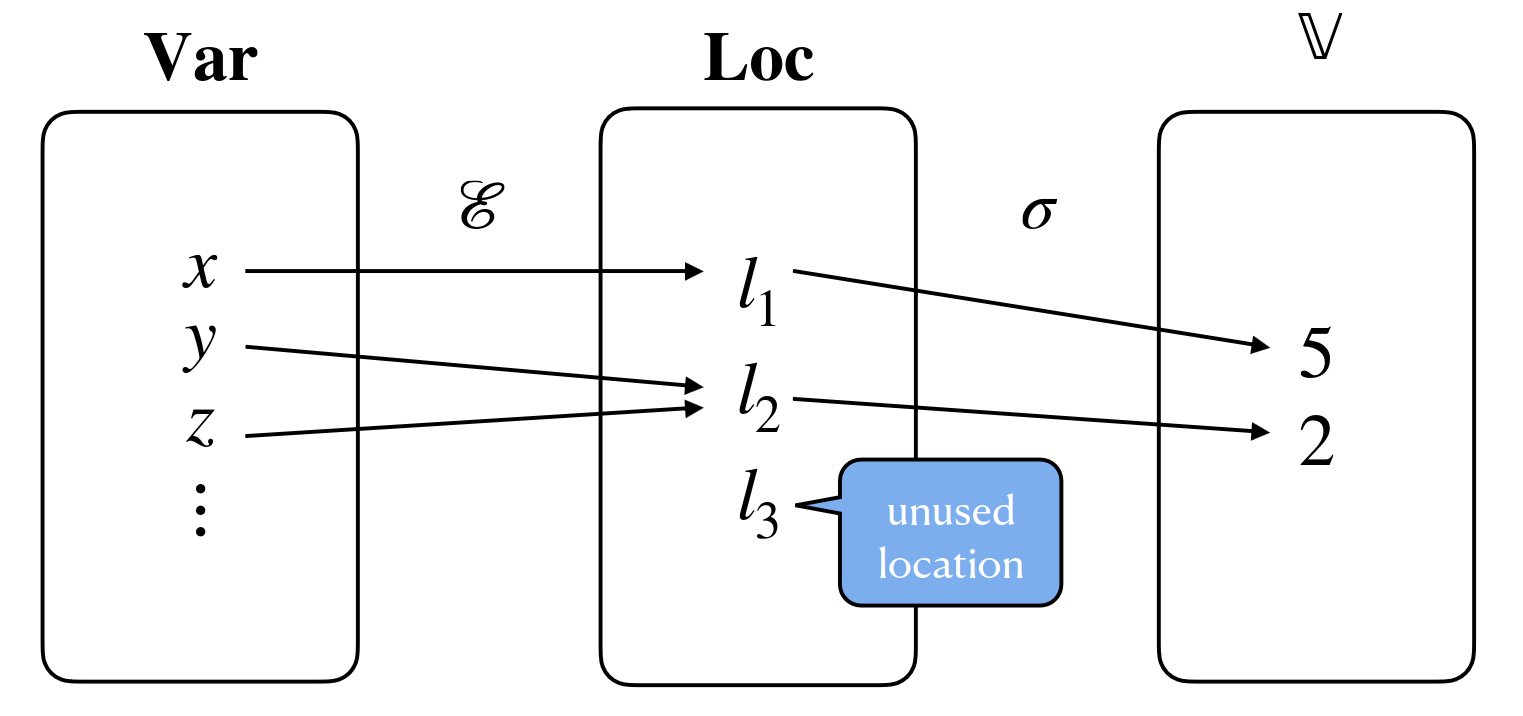
\includegraphics[width=\textwidth]{Files/Billeder: Design/ENVMODEL.png}
    \caption{Visualization of Environment-Store Model \cite{SS_lecture_12}}
    \label{fig:EnvModel}
\end{figure}

\noindent In order to understand the semantics that is defined using the environment-store model, we need to have three definitions in place.

\begin{itemize}
    \item \textbf{Variable Environment:} A partial function that tells which storage location each variable is bound to \cite{SS_lecture_12}. The set of variable environments will be defined as the following:
    \begin{table}[H]
    \centering
    \begin{tabular}{l|l}
    \textit{Single Instance} & \textit{Set of Variable Environments} \\
    $Env_v : \textbf{Var} \rightharpoonup \textbf{Loc}$       & $\mathbf{Env_V} = \textbf{Var} \rightharpoonup \textbf{Loc}$                          
    \end{tabular}
    \end{table}

    \item \textbf{Function Environment:} Describes the content of function name bindings. Essentially the name of a function is bound to the statements and parameters inside of its block, as well as the variable environment given at that time, in order to keep the variable environment statically bound. The function environment will be denoted as the following:
    \begin{table}[H]
    \centering
    \begin{tabular}{l|l}
    \textit{Single Instance} & \textit{Set of Function Environments} \\
    $Env_f : \textbf{Func} \rightharpoonup \textbf{Stm} \ \times \ \textbf{Var} \ \times \ \mathbf{Env_V}$       & $\mathbf{Env_F} = (\textbf{Func} \rightharpoonup \textbf{Stm} \ \times \ \textbf{Var} \ \times \ \mathbf{Env_V})^*$                         
    \end{tabular}
    \end{table}
        
    \item \textbf{Store:} A partial function which describes the content of a storage cell corresponding to a given location \cite{SS_lecture_12}. It is important to note that this is only applicable in relation to variable environments. The store acts as the memory of the model. It will be noted as the following: 

    \begin{table}[H]
    \centering
    \begin{tabular}{l|l}
    \textit{Single Instance} & \textit{Set of all stores} \\
    $\sigma : \textbf{Loc} \rightharpoonup \mathbb{V}$       & $\textbf{Sto} = \textbf{Loc} \rightharpoonup \mathbb{V}$            
    \end{tabular}
    \end{table}
    \begin{center}
        $Where \ \mathbb{V} \in \mathbb{R} \cup \{\mathbb{T}, \mathbb{F}\} \cup \textbf{Txt}$
    \end{center}

\end{itemize}

\noindent When each of these definitions are used in the following sections where the semantics of \lang are explained, they will be referred to as the symbols written in each of their single instances. For the model to work, the abstract set \textbf{Loc} of locations is assumed to exist, a single instance of a location is denoted by $l$. The function $nxt(l) = 1 + l$, can be called whenever the next available location needs to be retrieved\cite{SS_lecture_12}.

\subsection{Transition Systems for \lang} \label{TSytstem:Lang}

The necessary theory to understand the big-step semantics has now been described and we will explain the transition system for \lang in this subsection. The semantics will be based on the formation rules in section \ref{tab:formationrules}. The chosen semantic examples are based on complexity and equivalence. \\

\newpage\noindent
\textbf{Expressions}

\noindent
The format for expressions is the following $\sigma \circ Env_v \vdash e \rightarrow _{\textbf{Exp}} v$. The expression category will be derived first, since it is one of the fundamental levels of derivation, and is used in many of the other categories.  
\noindent
The set of configurations for expressions in \lang is that of any expression and variable type.
\\

\( \Gamma_{\textbf{Exp}} = \textbf{Exp} \cup \textbf{Num} \cup \textbf{Dec} \cup \textbf{Txt} \cup \textbf{Bool}  \) \\

\noindent The terminal configurations on the other hand are almost the exact set, but where all expressions have been evaluated to one of the base types. The terminal configurations can be formally described as the following definition \\

\( T_{\textbf{Exp}} = \textbf{Num} \cup \textbf{Dec} \cup \textbf{Txt} \cup \textbf{Bool} \) \\

\noindent With this in mind, a couple of examples of how expressions are derived can be seen in the following definitions.

\begin{equation}
    (VAR_{BS})\frac{\sigma(Env_v(x)) = \ v}{\sigma \circ Env_v \vdash x \rightarrow _{\textbf{Exp}} v } \ \
        if \ Env_v[x \rightarrow l] \ and \ \sigma[l \rightarrow v]
\end{equation}

\begin{equation}
\begin{split}
    (\star_{BS})\frac{\sigma \circ Env_v\vdash e_1 \rightarrow _{\textbf{Exp}} v_1 \ \ \sigma \circ Env_v \vdash e_2 \rightarrow _{\textbf{Exp}} v_2 }{\sigma \circ Env_v \vdash e_1 \star e_2 \rightarrow \ _{\textbf{Exp}} \ v_1 \star v_2 } \\
    Where \ \star \in (*, -, >, \geq, \leq, <, and, or, is, is \ not)
\end{split}
\end{equation}

\noindent $(VAR_{BS})$ is the derivation of an applied variable, which looks up the value of the variable in the store, which is connected to the variable environment through the location. The equation under the line can be informally read as, "In the composite function $\sigma \circ Env_V$, the variable $x$ evaluates to the expression $v$. $(\star_{BS})$ describes the derivation of the transition that most of the arithmetic and boolean expressions evaluate. The addition operator (+) is not included in $(\star_{BS})$ because it derives differently based on whether the expressions are of type \textbf{Txt} or type \textbf{Num} / \textbf{Dec}. The derivation for addition is showcased in the appendix \ref{appendix:SOS} \\

\noindent \textbf{Declarations} \\

\noindent The next formation rules are the declarations. This includes both declaration of a function and the declaration of a statement. It is important to note that declarations can also be considered statements, however because of their fundamental significance, they are displayed separately. The format of a function declaration is the following $Env_v, Env_f \vdash _l \langle D_F, \sigma \rangle \rightarrow \sigma'$. How the function environment is updated when a new function is declared will be shown when defining the transition for function declaration. \\

\noindent The set of configurations for a function declaration is the following: \\

$\Gamma _{\mathbf{D_F}} = \textbf{DecFunc} \times \textbf{Sto}$ \\

\noindent The set of terminal configurations for a function declaration which the above set can transition to, is the following: \\

$T_{\mathbf{D_F}} = \textbf{Sto}$ \\

\noindent Given the above configurations, the transition relation can be defined through a derivation. The derivation can be seen in definition \ref{funcDec_BS}.

\begin{equation} \label{funcDec_BS}
    (FUNCDEC_{BS})\frac{Env_v, \ Env_f[f \ \mapsto  (S, \ x_1, \ ..., \ x_k, \ Env_v)] \vdash _l \ \langle S_2, \ \sigma \rangle \rightarrow \ \sigma' }{Env_v, \  Env_f \vdash _l \ \langle function \ f(T_1 x_1, ... \ , T_k x_k) 
\ return \ T \{ S_1 ; return \ e\} ; \ S_2 , \ \sigma \rangle \rightarrow \ \sigma'}
\end{equation} 
\begin{center}
    $Where \ S = S_1 ; \ return \ e$
\end{center}

\noindent The function name $f$ is appended to the function environment where it maps to the statement $(S)$ within the block of the function, along with all the formal parameters $(x_1, ..., x_k)$, and finally the variable environment $(Env_v)$ given at the time of declaration. Some of the formation rules have an additional statement at the end of its process, which allows us to show semantically how a given environment is updated when used in the continuation of the program. \\

The format for variable declarations is $Env_v, Env_f \vdash _l \langle D_V, \sigma \rangle \rightarrow \sigma' $. The configurations are the same as the function declarations configurations, but where we use the \textbf{DecVar} category instead of the \textbf{DecFunc}. The transition relation is shown in definitions \ref{VARDEC1_BS} and \ref{VARDEC2_BS}.

\begin{equation} \label{VARDEC1_BS}
    (VARDEC1_{BS})\frac{\sigma \ \circ \ Env_v \ \vdash \ e \ \rightarrow _{\textbf{Exp}} \ v \ \ \ Env_v[x \ \mapsto \ l], Env_f \ \vdash _{nxt(l)} \langle S, \sigma[l \ \mapsto \ v] \rangle \ \rightarrow \ \sigma'}
    {Env_v, Env_f \ \vdash _l \ \langle T \ x \ = \ e \ ; \  S \ , \ \sigma \rangle \ \rightarrow \ \sigma'}
\end{equation}

\begin{equation} \label{VARDEC2_BS}
    (VARDEC2_{BS})\frac{Env_v[x \ \mapsto \ l], Env_f \ \vdash _{nxt(l)} \langle S, \sigma[l \ \mapsto \ d(T)] \rangle \ \rightarrow \ \sigma'}
    {Env_v, Env_f \ \vdash _l \ \langle T \ x \ ; \  S \ , \ \sigma \rangle \ \rightarrow \ \sigma'}
\end{equation}

\begin{table}[H]
\centering
\begin{tabular}{lll}
\textit{Where} & & \\
\textit{d(number)}  & = & 0      \\
\textit{d(text)}    & = & ""     \\
\textit{d(boolean)} & = & $\mathbb{F}$ \\
\textit{d(decimal)} & = & 0.0    \\
\textit{d(list(B))} & = & {[}{]}
\end{tabular}
\caption{Default values for all variable types}
\label{tab:defaultTypeValues}
\end{table}

\noindent The two variable declarations are fairly similar, $(VARDEC1_{BS})$ allows the programmer to assign a new variable a value immediately, whereas $(VARDEC2_{BS})$ is simply a declaration that a variable is now applicable. In both transitions, we update the variable environment with the new variable and the store with the new value. A declaration of an empty variable must be given a default value, which is seen in table \ref{tab:defaultTypeValues}. This is to avoid any errors that might occur when dealing with a variable that does not have a value within its domain. To better show how the updated environment is used, a statement $(S)$ is attached to both formation rules as previously done in the $(FUNCDEC_{BS})$ in definition \ref{funcDec_BS}. \\

\noindent \textbf{Statements}
%| DV | x:add(e1 , ... , ek) | x:insert(e , n) | x:valueOf(n) | x:indexOf(e) | if(e) { S } | If(e) { S } Else { S } | repeat (n) times { S } | repeat while (e) { S } | repeat for each (B x in x) | call f (e1, ... , ek) | ε

\noindent The transition rules for statements are in the format $Env_v, Env_f \vdash \langle S, \sigma \rangle \rightarrow  \sigma '$.  Statements are essentially just ways to update the store, this is denoted by the sigma prime notation $(\sigma')$ on the right-hand side of the arrow. Some of the most essential statement derivations are shown here in the report, the rest can be found in appendix \ref{appendix:SOS}. \\

Similarly to all the other syntactical categories, the set of configurations needs to be defined for statements. Statements should be transitioned from a pair, given a statement and a store, into just an instance of a store. This is showcased in the following definitions. \\

$\Gamma _{\mathbf{Stm}} = \mathbf{Stm} \times \mathbf{Sto}$ \\

\noindent This will transition into the terminal configurations given as the following definition. \\

$T_{\mathbf{Stm}} = \mathbf{Sto}$ \\

\noindent The first derivation shown is the compositional statement. This derivation is essential for allowing the program to be infinitely long, as it implements a recursive element to the statement category. The derivation is shown in definition \ref{COMP_BS}.

\begin{equation} \label{COMP_BS}
    (COMP_{BS})\frac{Env_v,\ Env_f \vdash _l \langle S_1, \sigma \rangle \rightarrow  \sigma ' \ \ \ Env_v,\ Env_f \vdash _l \langle S_2, \sigma' \rangle \rightarrow \sigma ''}{Env_v, Env_f \vdash _l \langle S_1;S_2, \sigma \rangle \rightarrow  \sigma ''}
\end{equation}

\noindent In $(COMP_{BS})$ the two statements are separated above the line, so they can each be individually derived. The key observation to make with this derivation is how the store is updated and used. The second statement will use the updated store from the first statement. The final store for the complete derivation is below the line $\sigma''$, as it is the updated store after $S_2$ has been derived. \\ 

The next statement described is the assignment statement. The assignment is used whenever updating an existing variable. The point of interest with the $(ASS_{BS})$ derivation is how the store is updated. The derivation can be seen in definition \ref{ASS_BS}. 

\begin{equation} \label{ASS_BS}
    (ASS_{BS})\frac{\sigma \circ Env_v \ \vdash\ e\ \rightarrow _{\mathbf{Exp}} \ v}{Env_v, Env_f \vdash _l \langle x = e,\ \sigma \rangle \rightarrow \sigma[Env_v(x)\ \mapsto v]}
\end{equation}

\noindent The expression $e$ is evaluated given the variable environment and store. In the transition below the line, we note that only the store has updated the value of the location of $x$. The variable environment remains the same, this is because the variable $x$ is assumed to already exist in the environment. \\

A function call can also be used as an assignment but is one of the more complex derivations of the statement category. It is important to note that a function call originally also could be considered an expression because the function call can return an expression. However, to simplify the operational semantics a function call is only included as a statement. This simplifies the operational semantics since we no longer need to include the \textbf{sto} in our \textit{terminal configurations} for the expression category. This change can be made as the result will be equivalent, shown in listing \ref{list:eqvivCallF}. The listing shows two syntactically correct function calls, however, the second example cannot occur in the abstract syntax. 

\begin{lstlisting}[language = scriptkid, label={list:eqvivCallF},caption=Example of equivalence of function call as statement and expression]
comment: Function call as statement;
number x;
number y = 0;
function f(number i) return number {
    return i+1;
}
x = call f(y);
if (x > 0) {}

comment: Function call as expression;
number x;
number y = 0;
function f(number i) return number {
    return i+1;
}
if (call f(y) > 0) {}
\end{lstlisting} \\

\begin{equation}
\label{FUNCEXP_BS}
\resizebox{1.1\textwidth}{!}{
(FUNCEXP_{BS})\frac{\begin{array}{c} Env_f(f) \ = \ (S, x_1, ... , x_k, Env_v') \ \ \ \sigma \circ Env_v \vdash 
\ e_i \ \rightarrow _{\textbf{Exp}} \ v_i \\  Env_v'[x_1 \mapsto l_1][x_2 \mapsto l_2]...[x_k \mapsto l_k], Env_f\vdash _{nxt(l)}
\langle S, \sigma[l_1 \mapsto v_1]...[l_k \mapsto v_k] \rangle \rightarrow \ \sigma'
\end{array}}
{Env_v, Env_f \vdash_l \ \langle 
x \ = \ call \ f(e_1, \ ... \ , \ e_k), \ \sigma \rangle \rightarrow \ \sigma'}}
\end{equation}
\begin{center}
 $Where \ i = 1...k $ \\ 
$if \ l_1 = l \ , \ l_{i+1} = nxt(l_i)$ \\     
\end{center}

\noindent The derivation for $(FUNCEXP_{BS})$ is shown in definition \ref{FUNCEXP_BS}. Everything above the line should be interpreted as a single long equation. It transitions the call of a function, used as an assignment to a variable. Above the line from left to right, it starts by deriving the function call into its representative statement, denoted by the $S$ within the angled brackets. The transition also assumes an updated variable environment $Env_v'$ where all the actual parameters from the call have been updated. The rest of the derivation above the line consists of the function name being associated in the function environment $Env_f(f)$ with its applied statements and formal parameters. Lastly, the expressions given as actual parameters are evaluated. \\

Next is the list operations. In definition \ref{LISTADD_BS} the list addition operation is displayed. The addition operation allows a programmer to append any amount of expressions at the end of the list. 

\begin{equation} \label{LISTADD_BS}
    (LISTADD_{BS})\frac{\sigma \ \circ \ Env_v \ \vdash \ e_i \ \rightarrow _{\textbf{Exp}} \ v_i}
    {Env_v, Env_f \ \vdash _l \ \langle \ x:add(e_1, ... , \ e_k), \ \sigma \rangle \ \rightarrow \ \sigma[Env_v(x) \ \mapsto \ L']}
\end{equation}
\begin{center}
$Where \ i = 1...k \ and  \ Env_v[x \ \mapsto \ l]$ \\
$and \ L' \ = \ L \ where \ the \ values \ v_i \ is \ appended \ to \ the \ end \ of \ the \ list$ \\
\end{center}


\noindent In $(LISTADD_{BS})$ we derive the statement by evaluating every expression into its value, and then the store is updated by updating the values of $x$, under the assumption that $x$ is a list. Similar to the $(ASS_{BS})$ derivation, the variable environment is not updated, since it is assumed that the list $x$ already exists in that environment. \\

The last two statements whose derivation will be shown are the \textit{if-true} statement which can be seen in definition \ref{IF-TRUE_BS} and a loop variant displayed in definitions \ref{REPEATTRUE_BS} and \ref{REPEATFALSE_BS}.

\begin{equation} \label{IF-TRUE_BS}
    (IFTRUE_{BS})\frac{Env_v,\ Env_f\ \vdash\ _l \langle S,\ \sigma \rangle\ \rightarrow\ \sigma '\ \ \ \sigma \circ Env_v \vdash e \ \rightarrow_{Exp} \mathbb{T}}{Env_v, Env_f \vdash _l \langle if (e)\ \lbrace S \rbrace , \ \sigma \rangle \rightarrow\ \sigma '}
\end{equation}

\noindent The $(IFTRUE_{BS})$ derives the statement 
$S$ in the case that the given expression $e$ derives to the Boolean value \textit{true}. The expression evaluates to a Boolean in this case since we define the given expression in an $if$ statement to be of Boolean type.
Since a Boolean also can derive to \textit{false}. It is also necessary to have a semantic derivation for the $if$ statement in case the expression evaluates to false, displayed in appendix \ref{IF-FALSE_BS}. \\

\begin{equation} \label{REPEATTRUE_BS}
    \resizebox{1.1\textwidth}{!}{
    (REPEATX-\mathbb{T}_{BS})\frac{Env_v, Env_f \ \vdash _l \ \langle S, \ \sigma \rangle \ \rightarrow \ \sigma' \ \ \ \sigma \circ Env_v \ \vdash n \ \rightarrow  ̣_{\textbf{Num}} \ v \ \ \ Env_v, Env_f \ \vdash _l 
    \ \langle repeat \ (v \ - \ 1) \ times \ \{ \ S \ \}, 
    \ \sigma' \rangle \ \rightarrow \ \sigma''}{Env_v, Env_f \ \vdash _l \ \langle repeat \ (n) \ times \ \{ \ S \ \}, 
    \ \sigma \rangle \ \rightarrow \ \sigma''}}
\end{equation}

\noindent $Where \ n > 0$

\begin{equation} \label{REPEATFALSE_BS}
    (REPEATX-\mathbb{F}_{BS})\frac{\sigma \ \circ \ Env_v \vdash \ n \ \rightarrow _{\textbf{Num}} \ 0}{Env_v, Env_f \ \vdash _l \ \langle repeat \ (n) \ times \ \{ \ S \ \}, 
\ \sigma \rangle \ \rightarrow \ \sigma'}
\end{equation}

\noindent $Where \ n = 0$ \\

\noindent The purpose of the loop variant derived in the above definitions, is to repeat a statement, a set amount of times. This loop variant can be useful, when wanting to repeat something, regardless of how the environment changes after each iteration. It is necessary to have two derivations of this one loop variant because two different outcomes are possible which change the flow of the program. The first transition $(REPEATX-\mathbb{T}_{BS})$, derives the loop given $n > 0$, indicating that the loop should execute the statement. In order to repeat the loop we derive the exact same statement above line, but where the number now is subtracted by 1. Notice that the updated store $\sigma'$ derived from the statement, is then used as the input store of the next loop iteration. When the loop counter hits 0, the $(REPEATX-\mathbb{F}_{BS})$ derivation should be activated, which ends the loop, when the number $n$ is evaluated to 0.

\subsection{Abstract Syntax Tree Design} \label{ASTDesign}
An Abstract Syntax Tree (AST) is an abstract representation of a parse tree. Parse trees are derived from the CFG, and an abstract syntax tree is instead derived from the abstract syntax described in table \ref{tab:formationrules}. An AST contains nodes but without the syntactic details and unnecessary in-between steps, and therefore more abstract. The nodes are mostly decided by looking at the CFG and imagining the shortest possible way to represent the same tree. In figure \ref{ASTNodes} all the AST nodes designed for \lang can be seen. The implementation of the AST in the compiler is described in the next chapter. 
%https://en.wikipedia.org/wiki/Abstract_syntax_tree

\begin{figure}[H] 
    \begin{center}
        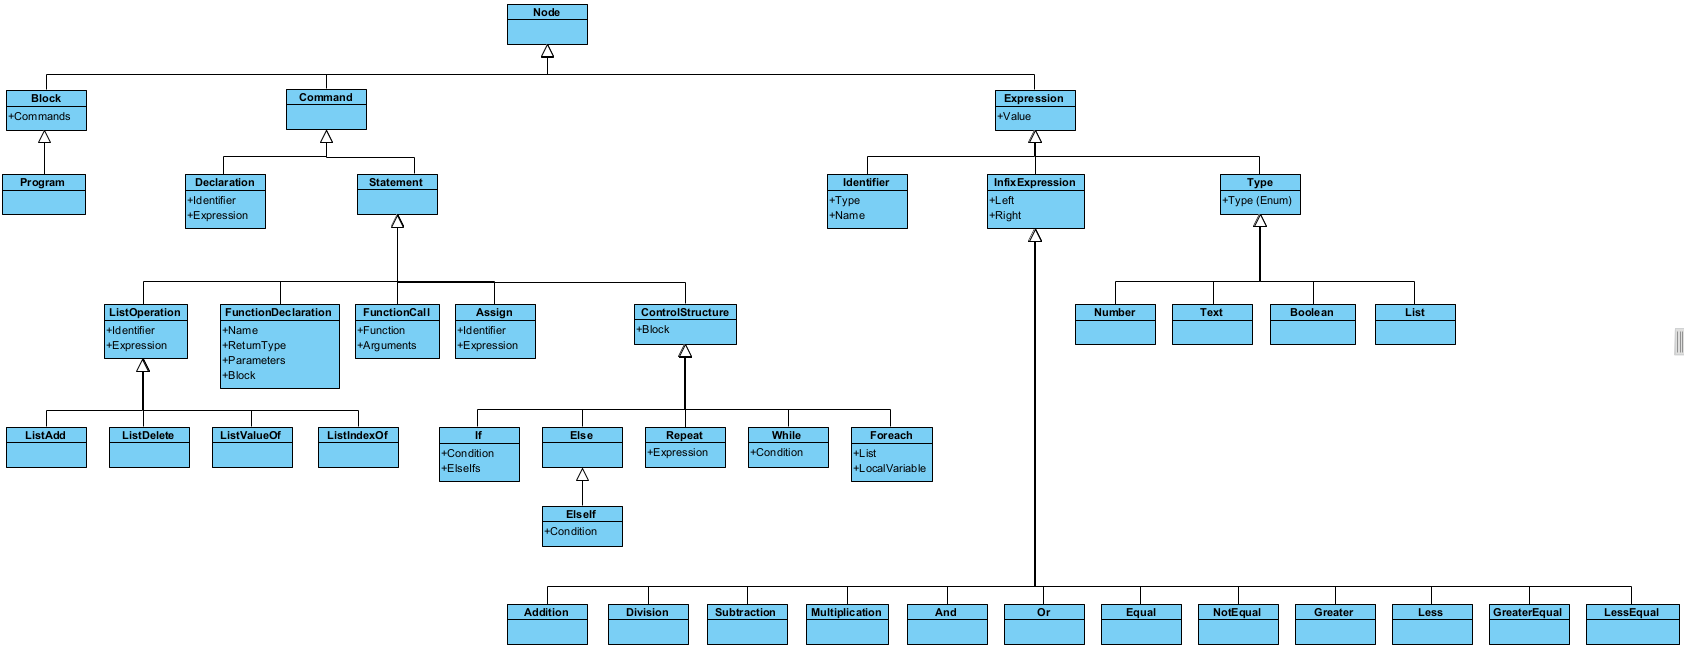
\includegraphics[width=1.5\textwidth, angle=90]{Files/Billeder: Design/ASTNodes.png}
    \end{center}
    \caption{The AST nodes in \lang represented as a class-diagram.}
    \label{ASTNodes}
\end{figure}

\chapter{Implementation}\label{ch:implementation}
With the language design settled in chapter \ref{ch:language_design}, this chapter documents the implementation of the \lang compiler. It touches on how the compiler is structured, justification of the choices made in the process, and documentation with code snippets of the compiler implementation.

\section{Compiler Phases}
The main phases of a compiler are 'Syntax Analysis', 'Contextual Analysis', and 'Code Generation'. In some of these phases, the visitor pattern is mentioned, which is further described in section \ref{lab:visitorPattern}. In this section, these phases are explained and described below.

\subsection{Syntax Analysis}
\noindent\textbf{Lexer:} The first part of the syntax analysis is the lexer, also known as the scanner. The lexer processes the input which is a stream of characters in the source language, and divides them into tokens. If a combination of characters does not match any token in the Lexer, an error is reported \cite{SPO_Topic_3}.\\

\noindent\textbf{Parser:} During Syntax Analysis the tokens get processed into a Parse Tree, using the CFG designed in section \ref{CFGForLang}. The tokens are checked to see if they match the defined grammar rules. If no grammar rules match a sequence of tokens, an error is reported \cite{SPO_Topic_3}. \\

\noindent
\textbf{AST:} Using the Parse Tree, an AST is generated to reduce the size of the tree by simplifying details. The AST nodes are designed in section \ref{AST}. The compiler goes through each grammar rule in the Parse-Tree using the visitor pattern and converts the Parse-Tree into AST nodes \cite{SPO_Topic_3}. 

\subsection{Contextual Analysis}
\noindent \textbf{Symbol Table:} To create a Symbol Table, the AST is iterated through a visitor pattern. 
In the Symbol Table, each scope containing its declared variables is stored. The Symbol Table also checks for scope issues and improper usage of declared variables and reports any error if so \cite{SPO_Topic_3}.\\

\noindent\textbf{Type Checker:} The Type Checker uses the AST and the Symbol Table to check for any type-related errors. This can be done using the visitor pattern \cite{SPO_Topic_3}. \\
%For example, the Type Checker will check if the condition of an if-statement evaluates to a boolean-value. \\

\noindent\textbf{Decorated AST:} When type-checking each node in the AST, additional information like type information and symbol table entries, can be added, generating a decorated AST. However, it is not necessary to create a decorated tree. It depends on the requirement for the compiler \cite{SPO_Topic_3}.

\subsection{Code Generation:} Finally the compiler goes through Code Generation. Code Generation once again uses the visitor pattern. In this phase, instructions based on the decorated AST nodes are generated. These instructions get translated to the target language of the compiler \cite{SPO_Topic_3}.

\section{\lang compiler} \label{peakCompiler}
To create the \lang compiler, these three compiler phases are implemented. The rest of this chapter will describe the implementation of syntax analysis, contextual analysis, and code generation. \\

\begin{figure}[H] 
    \begin{center}
        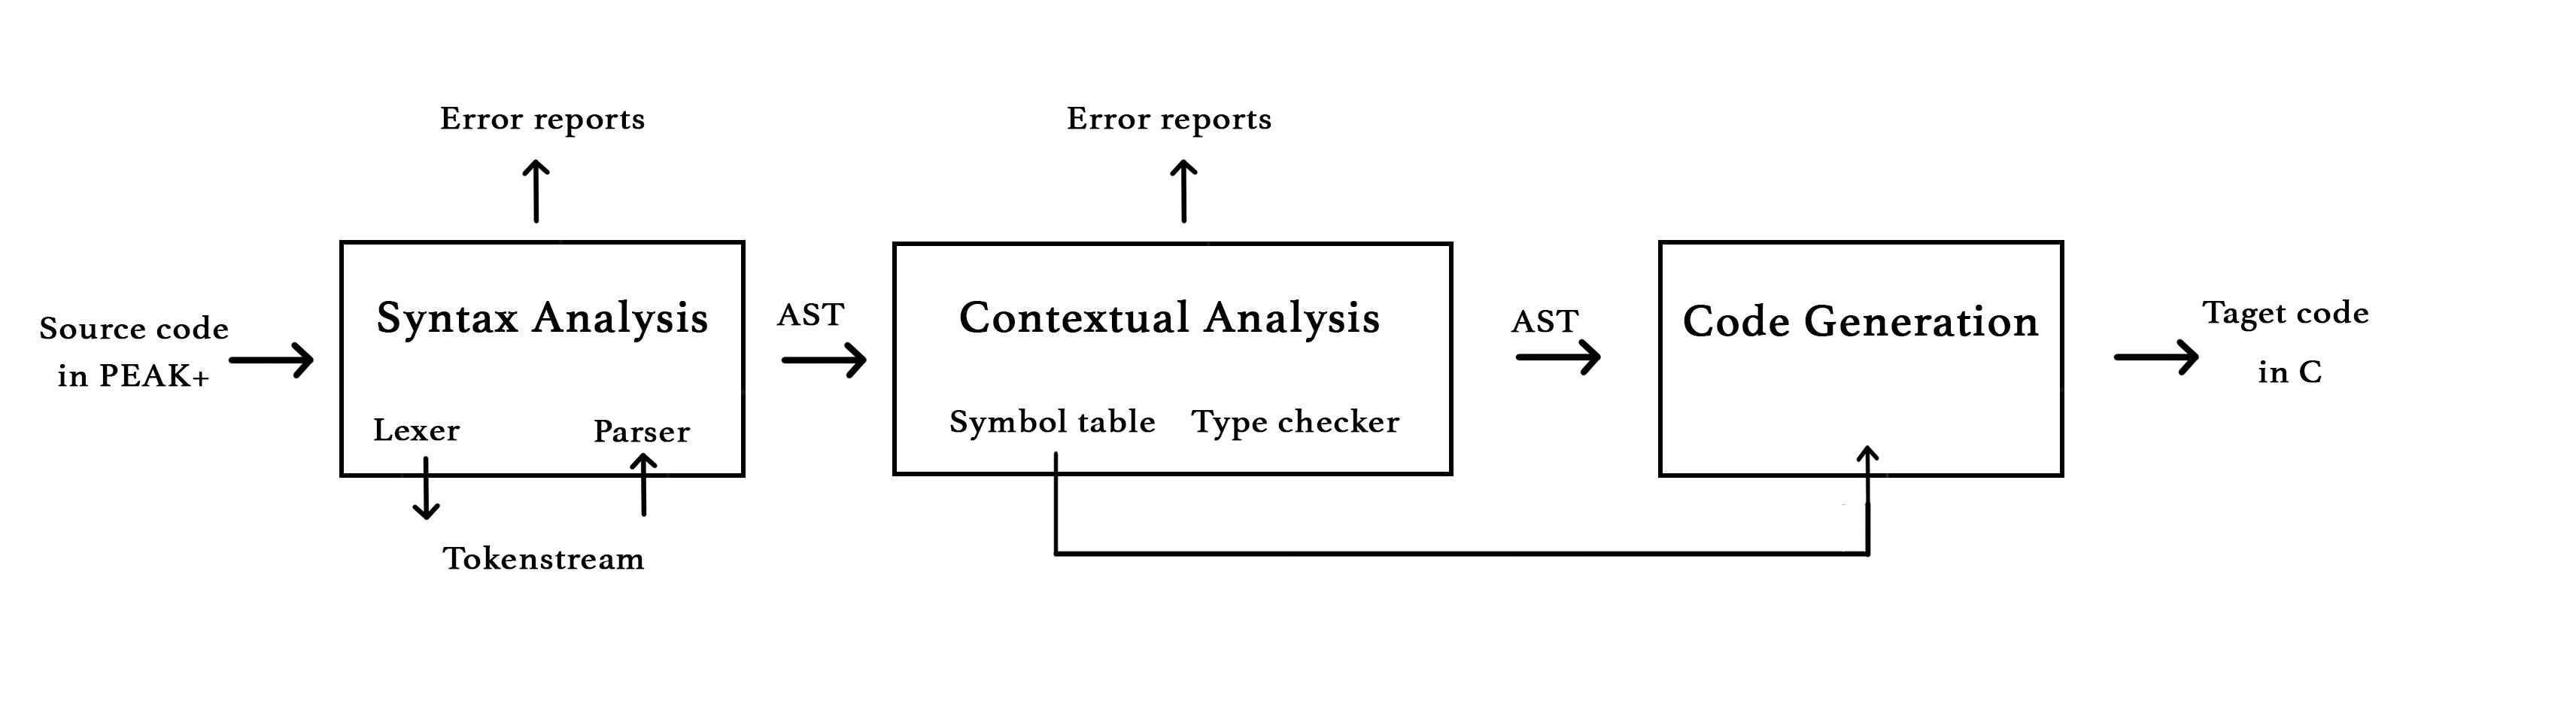
\includegraphics[width=1\textwidth]{Files/Billeder: Impl/OverviewCompiler.jpg}
    \end{center}
    \caption{Overview of the PEAK+ compiler}
    \label{I:Figurue:PEAKCompiler}
\end{figure}

\noindent As displayed in figure \ref{I:Figurue:PEAKCompiler} which shows an overview of the \lang compiler, the input to the lexer is the source code written in \lang. The lexer generates the token stream that the parser uses to generate the AST. Then the scope rules are checked in the symbol table, followed by type checking. The \lang compiler will not generate a decorated AST in the contextual analysis phase. Since \lang is a simple language, there is no need for decorating the AST before translating it into the target code. The target code for \lang is the C programming language. One of the reasons C is chosen is because of its flexibility, which makes it easier to adjust to the semantics of \lang, more details on the reasons behind C as the target code is explained in section \ref{I:CodeGeneration}.

\subsection{Deciding Compiler Language} \label{I:TargetLanguage}
In order to best implement a visitor pattern later on in development, an object-oriented language is needed. The visitor pattern is explained further in section \ref{lab:visitorPattern}. For this reason, the \lang compiler is going to be developed in C\#. This is also because C\# is a language that the group is acquainted with as well as how the project organization works in C\#. 

\section{Syntax Analysis}\label{I:SyntaxAnalysis}
Syntax Analysis is the first phase of the compiler which ends up generating an Abstract Syntax Tree (AST). This section will cover the theory of the parser algorithm followed by the implementation in the \lang compiler including the Parser Generator, and how the AST has been built. 

\subsection{Parsing Theory}
When a compiler translates source code, the parser defines the structure of the code by producing a parse tree. The basis for creating the parse tree is the token stream created by the lexer. The Lexer converts the source code characters into specified tokens. Lexical grammar uses regular expressions to define the grammar rules of a token. As displayed in figure \ref{I:Figure:ParsetreProcess}, the lexer, for example, translates the source code "12 + 23" into the \textit{Num}, \textit{Plus}, and \textit{Num} tokens. The parser uses this token stream to produce the parse tree by using the correlated CFG production rules. Implicit in the displayed example, a lexer rule will exist, specifying that a sequence of digits corresponds to the \textit{Num} token, the plus symbol corresponds to the \textit{Plus} token, and that the correlated CFG production rules say that a program consists of an \textit{expr} and that a \textit{expr} can be a \textit{Num Plus Num} \cite{ParsingGuide}. 

\begin{figure}[H] 
    \begin{center}
        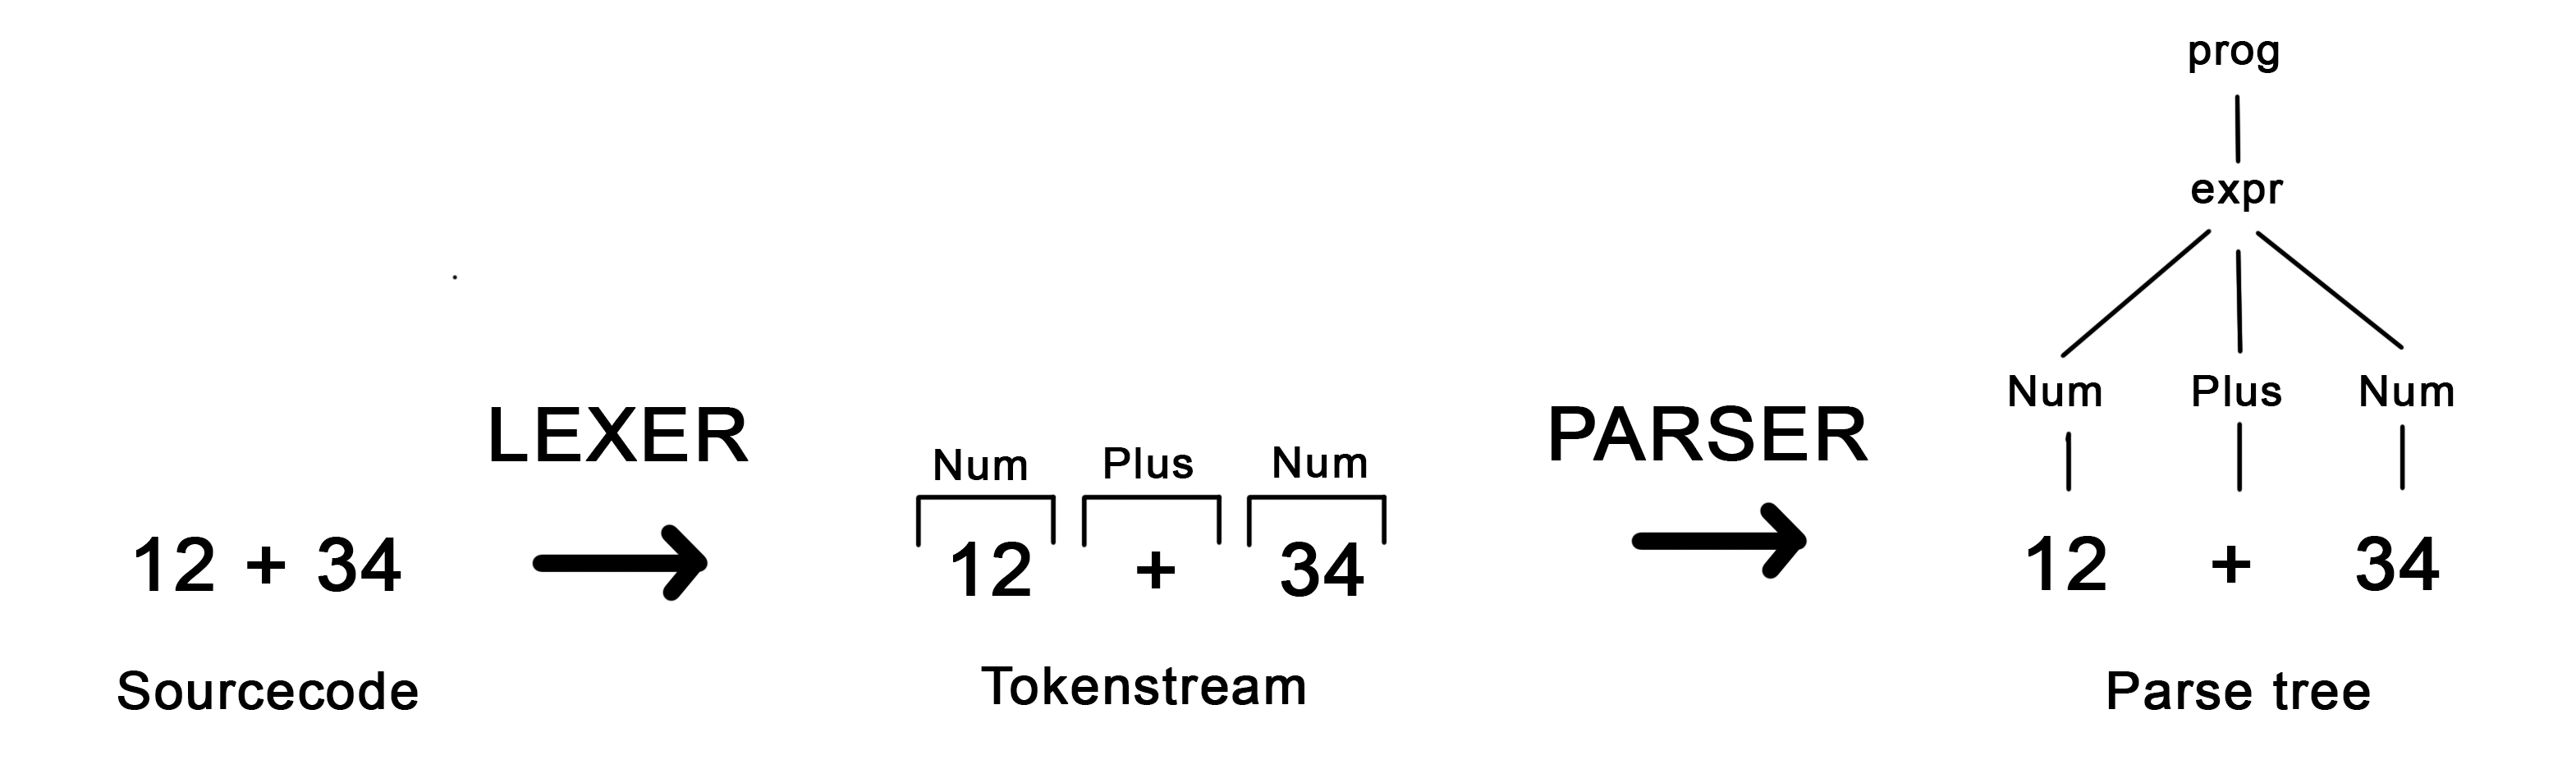
\includegraphics[width=1\textwidth]{Files/Billeder: Impl/parsing kopier.jpg}
    \end{center}
    \caption{An example of the process of translating source code into a parse tree}
    \label{I:Figure:ParsetreProcess}
\end{figure}

\noindent
By generating the parse tree, the parser checks the syntactic correctness of the source code. If the source code consists of syntax errors, error reports will be thrown. An example of syntactically correct but semantically incorrect code is displayed in listing \ref{list:SyntaxCodeFail}. The parser will not produce any errors, since the structure of the code is correct. But if the code is executed, it will fail since the variable x is not declared \cite{ParsingGuide}. 

\begin{lstlisting}[language = csharp, firstnumber=0, label={list:SyntaxCodeFail},caption=example of code with correct syntax but wrong semantics.]
int y = 10;
int sum = x + y;
\end{lstlisting}

\noindent
A parse tree is also called a concrete syntax tree (CST) and is traversed, from the root node of the tree, down to its subtrees representing smaller pieces of the code. The same principle applies to the AST, except that the CST is represented using the concrete syntax while the AST is more simplified and has fewer details that are not relevant for generating code \cite{ParsingGuide}. The difference between the two trees can be seen in figure \ref{I:Figure:ParseAST}. \\

\begin{figure}[H] 
    \begin{center}
        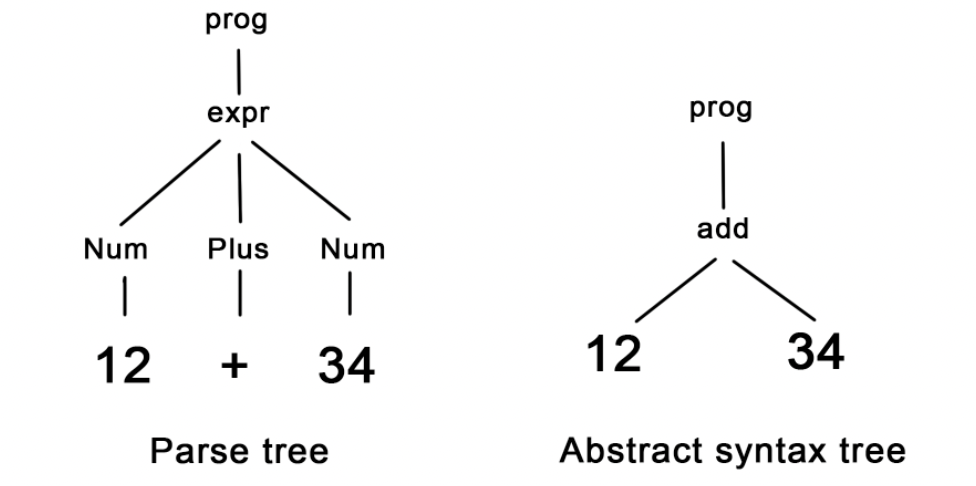
\includegraphics[width=0.7\textwidth]{Files/Billeder: Impl/parsetoAST.png}
    \end{center}
    \caption{Examples showing the difference between a CST and an AST}
    \label{I:Figure:ParseAST}
\end{figure}

\noindent
There are two approaches to parsing: top-down and bottom-up. A top-down parser traverses the tree from the root node until each leaf is visited. These are also known as LL(K) parsers (\textbf{L}eft-to-right read of input, \textbf{L}eftmost derivation). The k indicates the amount of lookahead the algorithm has, meaning how many tokens the parser has to include in its decisions of what grammar rule to follow. LL parsers are easy to implement but less efficient because they cannot handle left recursion grammar rules. However, there will always be an equivalent non-recursive grammar to a left recursive grammar, but the rewritten grammar rules can be more complex to understand, or need more lookaheads than the recursive grammar \cite{ParsingGuide}. \\

A bottom-up parser starts from the lowest part of the tree, ending at the root. The LR (\textbf{L}eft-to-right read of the input, \textbf{R}ightmost derivation) parser is a Bottom-up parser and is harder to implement, but can handle most grammars like left recursion. Both LL and LR parsers use parse tables that store information about the next action to take. For LR parsers, these tables can become large and complex. LALR (Look-Ahead, Left-to-right) is a variant of the LR parser and attempts to address the LR parsers issue by having large table sizes be more compact at the cost of potential conflicts with look-ahead \cite{ParsingGuide}. 

\subsection{Deciding Parser Tool}
Generating the parser can be done by hand or by using a parser generator tool. Using a tool can be faster and more accurate, especially with larger languages. A tool helps to reduce errors in the parser but often has some requirements for the grammar, like having to be LL(1). However, by generating the parser by hand, the developer has more control over how to handle the special requirements. Though, if the language's grammar is large and complex, it is a difficult and time-consuming task to write the parser by hand, leading to errors in the parser. Even though \lang is not that complex, our learning curve in this project means that changes probably would occur along the way. Because of the time consumption of having to rewrite the parser by hand several times, combined with our missing experience in writing a parser, we decided that a tool would be the appropriate choice. There are many different parser generators, and we researched JavaCup, SableCC, and ANTLR. \\

JavaCUP is an LALR bottom-up parser and generates a parser written in Java. Both SableCC and ANTLR are LL(k) and can generate a parser in multiple different languages. We prefer writing code in C\# and therefore the choice is between SableCC and ANTLR. After experimenting with getting both tools to work, ANTLR is the first to successfully work and to show a visual parse tree. In view of getting the parsing process started, ANTLR is therefore chosen as the parser generator. ANTLR can handle left recursion, and is an LL(*) parser meaning it can handle any amount of lookahead tokens \cite{ParsingGuide}.
%The source code for the \lang compiler can be found in the project GitHub repository called "P4-project" \cite{p4-project-rep}.

\subsection{Lexer}
ANTLR provides the ability to perform lexical analysis if it receives a lexer. Because of this, we are able to take our CFG and transform all terminal rules into keywords stored in the lexer. Some of the same terminal rules appear multiple times in the CFG, and therefore it is now easier to change all appearances of a terminal rule at once. Examples of keywords can be seen in listing \ref{list:Lexer_Example} for various list operations. In the lexer, definitions of regular expressions can be made. ANTLR uses different characters in its regular expressions compared to what normally is used. ANTLR for example uses \textit{\~}\ instead of \textit{\^} for excluding characters. Regular expressions are e.g. used in \lang for string values. In \lang, a string value starts with \textit{"} followed by any character which is not a \textit{"} and ends with \textit{"}. In ANTLR this regular expression can be seen in listing \ref{list:Lexer_Example} as 'STR' as well as some examples of other lexer rules. The full lexer can be seen in appendix \ref{list:ANTLR LEXER}.

\begin{lstlisting}[label={list:Lexer_Example}, captionpos=b, caption=Part of \lang's Lexer - CobraCompiler/ExprLexer.txt]
LISTADD: 'Add';
LISTIDXOF: 'IndexOf';
LISTREPLACE: 'Replace';
LISTVALOF: 'ValueOf';

COMM: 'comment:'~(';')*;
STR: '"' (~'"')* '"';
DEC: ('+' | '-')? [0-9]+'.'[0-9]+; 
INT: ('+' | '-')? [0-9]+ ;
ID: [a-zA-Z_][a-zA-Z_0-9]* ; 
WS: [ \t\n\r\f]+ -> skip ; 
\end{lstlisting}

\subsection{The Visitor Pattern}
\label{lab:visitorPattern}
In order to traverse a tree like the CST, a visitor pattern is required. A visitor pattern utilizes a depth-first search method to traverse the tree. It solves the problem of having to modify each class in a larger class structure whenever a change needs to be implemented. Instead, all visitor methods are contained within one class, and therefore only the functions have to be modified. This pattern is used in multiple phases of the \lang compiler, like when building the AST, creating the symbol table, type-checking, and generating the target code. Based on the context, a visit function in the pattern can return something different. For example, when building the AST, each visit function can return an AST node in order to build upon the AST \cite{VisitorWIKI}. An example of how the visitor pattern visits nodes using the depth-first search algorithm can be seen in figure \ref{fig:VisitorPattern_Example}.

\begin{figure}[H] 
    \begin{center}
        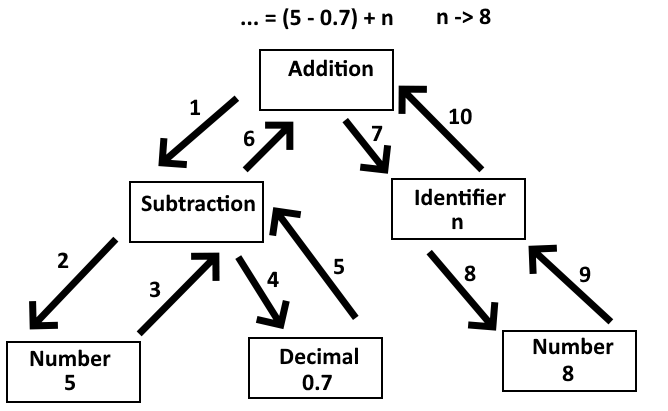
\includegraphics[width=0.6\textwidth]{Files/Billeder: Impl/VisitorpatternExample.png}
    \end{center}
    \caption{Example of the visitor pattern. The numbers above the arrows show which order the nodes are visited}
    \label{fig:VisitorPattern_Example}
\end{figure}

\subsection{Building the Abstract Syntax Tree}
Using ANTLR generates multiple classes including \textit{ExprParser}, \textit{ExprLexer}, and \textit{ExprParserBaseVisitor}. The order in which ANTLR generates the parser can be seen in listing \ref{list:Program_Parser}. First ANTLR uses an \textit{AntlrInputStream} class in order to turn the input into a stream of characters that ANTLR can use, seen on line 28. This stream of characters is used to instantiate a new \textit{ExprLexer} class which is assigned to the lexer variable on line 29. The lexer is then given to a \textit{CommonTokenStream} class which converts the lexer into tokens for the parser. This can be seen on line 30. The returned token stream is given to \textit{ExprParser} which finally generates the parser on line 31. From the parser, the start-node can be retrieved, which in our CFG is '\textit{program}'. This root is assigned to a variable called '\textit{cst}' (concrete syntax tree) on line 35. The '\textit{cst}' is required in order to build the AST.

\begin{lstlisting}[language = csharp, label={list:Program_Parser},firstnumber=28,caption=SymbolTable Class - CobraCompiler/Program.cs]
var inputStream = new AntlrInputStream(new StringReader(exprText));
var lexer = new ExprLexer(inputStream);
var tokenStream = new CommonTokenStream(lexer);
var parser = new ExprParser(tokenStream);
.
.
.
var cst = parser.program();
\end{lstlisting}

\noindent
Before building the AST, classes for each of the possible nodes must be created. '\textit{ASTNodes}' is a class that is created to contain these as well as the datatypes in \lang stored as an enumeration. These nodes are designed in section \ref{ASTDesign}. Each node inherits from an abstract class '\textit{ASTNode}' and through this, all nodes contain a property '\textit{Line}' which represents the line in the code where the node originates from. This property is used to inform the user where an error stems from if one occurs. \\

\noindent An example of the '\textit{AssignNode}' can be seen in listing \ref{list:ASTNodes}. In \lang, an assignment is written as $identifier = expression$. '\textit{AssignNode}' inherits '\textit{CommandNode}' since an assignment is a command. It contains an \textit{IdentifierNode} on line 54 and an \textit{ExpressionNode} on line 55.

\begin{lstlisting}[language = csharp, label={list:ASTNodes}, firstnumber=52, caption=SymbolTable Class - CobraCompiler/ASTNodes.cs]
internal class AssignNode : CommandNode
{
    public IdentifierNode Identifier { get; set; }
    public ExpressionNode Expression { get; set; }
}
\end{lstlisting}

\noindent
ANTLR generates the '\textit{ExprParserBaseVisitor}' class which is used by a class '\textit{BuildASTVisitor}'. It is used for building the AST by having '\textit{BuildASTVisitor}' inherit from it. '\textit{ExprParserBaseVisitor}' provides a visitor pattern for going through the symbols in the parse tree. It is a generic class and the generic type given is the return type of all visitor implementations of the class. This is in our case the class '\textit{ASTNode}'. The class contains unique visit methods for each non-terminal in \lang's CFG, as well as a general '\textit{Visit()}' method. In each of these methods, you are able to access the non-terminal '\textit{context}' which is used to get its children. The context can also be used to retrieve the line in which a rule occurred that can be stored in an AST node. The children can be used on the '\textit{Visit()}' method to visit the non-terminals children.\\

\noindent Using this, we can visit all children in the parse tree and return the correct ASTNodes. Each unique visit method has the following structure: 
\begin{itemize}
    \item All children are initialized at the top using the symbol's context
    \item If a node is to be returned, this also gets initialized here as '\textit{outputNode}'
    \item  One or more if-statements check for necessary syntax rules and visit the children
    \item At the bottom, the \textit{outputNode}'s properties are assigned, and it is returned
\end{itemize}

\noindent In order to test if '\textit{BuildASTVisitor}' returns the correct output, a '\textit{prettyPrint()}' function is run every time a new node is added to the AST. In order to correctly print the nodes at their respective levels of the AST, an indentation function '\textit{incrIndent()}' can be called. This function increments indentation for the next time a node is pretty printed. A function '\textit{decrIndent()}' decreases indentation again. An example of how it looks in the terminal, as a result of the implemented indentation can be seen in figure \ref{fig:pretty_print}. Because of time pressure, the pretty printer is not being maintained in the second iteration as it is mostly used to check if the output of the \textit{BuildASTVisitor} matches the source code. In the second iteration, we use debugging features to ensure that the resulting AST match.

\begin{figure}[H] 
    \begin{center}
        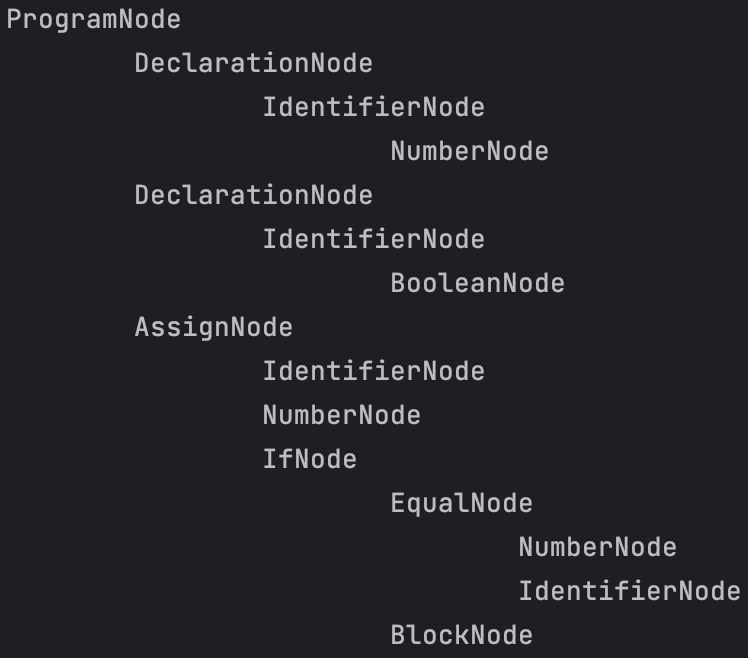
\includegraphics[width=0.5\textwidth]{Files/Billeder: Impl/pretty_print.png}
    \end{center}
    \caption{Pretty print example.}
    \label{fig:pretty_print}
\end{figure}

\noindent
An example of one of the visit functions can be seen in listing \ref{list:BuildASTVisitor}. This example is of a declaration rule in \lang's CFG which has the following structure: $dcl -> type \ ID \ ass \ SEMI;$. In the function, all children are initialized at the top on lines 139-142 as well as the node to return on line 144, which is a declaration node. On lines 149-152 an if-statement checks that the syntax is correct. Since a declaration-node contains an identifier-node we initialize this on line 154. An identifier node has a type node that is visited on line 159 and returned. This type node is assigned to the identifier node on line 160. On line 162, the declaration is checked for any assignments, since it is possible in \lang to have a declaration without any assignments. This assignment is assigned as an 'expression' to the '\textit{outputNode}' on line 167. The identifier node is also assigned on line 145 and the output is returned on line 170.

\begin{lstlisting}[language = csharp, firstnumber=132, label={list:BuildASTVisitor},caption=BuildASTVisitor Class - CobraCompiler/BuildASTVisitor.cs]
public override ASTNode VisitDcl([NotNull] ExprParser.DclContext context)
{
    //outputNode = DelcarationNode
    //visit(type) -> gets TypeNode
    //visit(ass) -> gets ExpressionNode
    //Type and Expression is assigned to an identifierNode
    //The identifierNode is assigned to the OutputNode
    var type = context.type();
    var ID = context.ID();
    var ass = context.ass();
    var SEMI = context.SEMI();

    var outputNode = new DeclarationNode() { Line = ass.start.Line };

    prettyPrint("DeclarationNode", context);
    incrIndent();

    if ((type != null) &&
        (ID != null) &&
        (ass != null) &&
        (SEMI != null))
    {
        var identifier = new IdentifierNode() { Line = ID.Symbol.Line };
        prettyPrint("IdentifierNode", context);
        incrIndent();

        identifier.Name = ID.ToString();
        var typeNode = (TypeNode)Visit(type);
        identifier.TypeNode = typeNode;

        if (ass.ChildCount > 0)
        {
            outputNode.Expression = (ExpressionNode)Visit(ass);
        }

        outputNode.Identifier = identifier;
    }

    decrIndent();
    return outputNode;
}
\end{lstlisting}

\newpage
\section{Contextual Analysis}\label{I:ContextualAnalysis}
Contextual Analysis is the phase of the compiler that usually "decorates" the AST to make a Decorated AST. It uses the Symbol Table and Type Checking to add any additional information which can for example be type information when performing type conversion. After the decorated AST is made the compiler enters the Code Generation phase. In \lang, we did not add type information to the AST until the second iteration, as it is necessary for the code generation to recognize for example if an addition-node is concatenating strings or adding two numbers.

\subsection{Symbol Table}
The symbol table created for \lang is developed in C\#. It is created using a '\textit{Scope}' class which represents the scopes of the program. This class can be seen in listing \ref{list:ScopeClass} and contains a stack of dictionaries, used for storing symbols and a reference to the scope '\textit{Parent}' (meaning its outer scope). It also stores a reference to the Block Node tied to the scope. In order to get a symbol from the dictionary when knowing its ID, the dictionary's key is the symbol's ID. This helps to get the symbol in constant time, which is more efficient for the compiler than iterating through all symbols until it finds a match. The Symbol class in listing \ref{list:SymbolClass} defines the properties of a symbol, which includes its name, type, and reference to the declaration node. The Type property is of type \textit{TypeEnum}, which is an enumerator that defines the possible types of symbols: number, text, boolean, decimal,  list\_number, list\_text, and list\_boolean.\\
The scope rules which the symbol table manages are described in section \ref{sec:scope_rules}.

\begin{lstlisting}[language = csharp, firstnumber=28, label={list:ScopeClass},caption=Scope Class - CobraCompiler/SymbolTable.cs]
public class Scope
{
    public Scope()
    {
        Symbols = new Dictionary<string, Symbol>();
    }
    public Dictionary<string, Symbol> Symbols { get; set; }
    public Scope Parent { get; set; }
    public BlockNode Block { get; set; }
}
\end{lstlisting}

\begin{lstlisting}[language = csharp, firstnumber=21, label={list:SymbolClass},caption=Symbol Class - CobraCompiler/SymbolTable.cs]
public class Symbol
{
    public TypeEnum Type { get; set; }
    public string Name { get; set; }
    public ASTNode Reference { get; set; }
}
\end{lstlisting}

\noindent
The SymbolTable class in listing \ref{list:SymbolTableClass} builds and stores the symbol table. Besides its 'Visit()' functions, the class provides six methods \textit{BuildSymbolTable()}, \textit{ProcessNode()}, \textit{NewScope()}, \textit{ExitScope()}, \textit{Insert()}, and \textit{Lookup()}. The \textit{BuildSymbolTable()} method takes the root of the AST as its input and processes each node in the tree using the visitor pattern. \\

The \textit{NewScope()} method is used when visiting a new block when building the symbol table. It takes a \textit{BlockNode} as a parameter, creates a new scope, and pushes it onto a stack. This stack keeps track of the current scope by storing it at the top. If possible, the parent of the scope is also set. The scope is also stored in a separate dictionary where each scope can be accessed using its \textit{BlockNode}. Finally, the blockNode which belongs to the now current scope, is stored.\\

The \textit{ExitScope()} method pops the top element of the scope stack to represent exiting a scope. This method is called when exiting a scope during the symbol table creation. \\

The Insert method takes a string \textit{name} and a \textit{TypeEnum} as its inputs and adds a new symbol to the current scope at the top of the stack. Insert is called when visiting a declaration node, as the newly declared variable needs to be stored in the symbol table. \\

The Lookup method takes a string \textit{name} and a \textit{BlockNode}. It starts at the scope belonging to the \textit{BlockNode} and searches outwards through each scope's dictionary for the requested symbol and returns it if found. If the symbol is not found, \textit{null} is returned and an error is reported. This function is called when meeting an Identifier node in the AST, which represents already declared variables.

\begin{lstlisting}[language = csharp, firstnumber=39, label={list:SymbolTableClass},caption=SymbolTable Class - CobraCompiler/SymbolTable.cs]
public class SymbolTable : ASTVisitor<ASTNode?>
{
    public Dictionary<BlockNode, Scope> _scopes;
    public Stack<Scope> _stackScopes;
    private ErrorHandler symbolErrorhandler;
    public BlockNode _currentBlock;
    .
    .
    .
    public SymbolTable(ErrorHandler errorHandler)
    {
        symbolErrorhandler = errorHandler;
        _scopes = new Dictionary<BlockNode, Scope>();
        _stackScopes = new Stack<Scope>();
    }
    public SymbolTable BuildSymbolTable(ASTNode astRoot)
    {
        Visit((ProgramNode)astRoot);
        return this;
    }
\end{lstlisting}

\begin{lstlisting}[language = csharp, firstnumber=232, label={list:Visit},caption=Visit(DeclarationNode node) - CobraCompiler/SymbolTable.cs]
public override ASTNode? Visit(DeclarationNode node)
{
    if (_reservedKeywords.Contains(node.Identifier.Name))
        node.Identifier.Name = $"{node.Identifier.Name}_";

    var sym = Lookup(node.Identifier.Name, _currentBlock);

    string underscores = "";
    while (sym != null)
    {
        underscores += "_";
        sym = Lookup($"{node.Identifier.Name}{underscores}", _currentBlock);
    }

    node.Identifier.Name += underscores;
    Insert(node.Identifier.Name, node.Identifier.TypeNode.Type, node);
    Visit(node.Expression);
    return null;
}
\end{lstlisting}

\noindent
\textit{NewScope()} in listing \ref{list:NewScope} creates a new scope in the symbol table. It takes a block node on line 75, which is associated with the scope, and assigns it to a new scope on line 78. If any scopes already exist, the scopes parent is assigned to the current scope at the top of the stack on lines 80-81. The scope is pushed onto a stack of scopes and added to a dictionary of scopes on lines 83-84. The current block is then updated to refer to the new scope block on line 85. The method uses \textit{\_stackScopes.Peek()} on the dictionary on lines 81 and 85 to retrieve the top element which is the current scope. This function is called when entering a new block of code, such as a function or loop. Variables declared within this block will only be visible within this scope and any nested scopes.

\begin{lstlisting}[language = csharp, firstnumber=75, label={list:NewScope},caption=NewScope() - CobraCompiler/SymbolTable.cs]
private void NewScope(BlockNode blockNode)
{
    var scope = new Scope();
    scope.Block = blockNode;

    if (_stackScopes.Count > 0)
        scope.Parent= _stackScopes.Peek();

    _scopes.Add(blockNode, scope);
    _stackScopes.Push(scope);
    _currentBlock = _stackScopes.Peek().Block;
}
\end{lstlisting}

\noindent
The method \textit{ExitScope()} in listing \ref{list:ExitScope} exits the current scope in the symbol table. It pops the top dictionary from the scope stack using the \textit{Pop()} method, effectively removing it from the symbol table on line 90. It also updates the current block to be that of the new current scope after popping the stack on lines 92-93. It does this if the block is not of type program-node as you can not go further out than the program-node. This method is called when exiting a block of code.

\begin{lstlisting}[language = csharp, firstnumber=89, label={list:ExitScope},caption=ExitScope() - CobraCompiler/SymbolTable.cs]
private void ExitScope()
{
    _stackScopes.Pop();
    if (_currentBlock is not ProgramNode)
        _currentBlock = _stackScopes.Peek().Block;
}
\end{lstlisting}

\noindent
The method \textit{Insert()} in listing \ref{list:Insert} inserts a new symbol into the symbol table. It takes three arguments: the name of the symbol, its type represented by a \textit{TypeEnum}, and the node of the declaration on line 98. Because of the scope rules defined in chapter \ref{ch:language_design}, the same name for a variable can not be defined within the same scope, only in separate scopes. Therefore \textit{Insert()} checks if the current scope contains the name of the variable being inserted on line 100. If it already exists, an error will be reported on line 102. If this is not the case, it adds a new entry to the dictionary using the name parameter as the key and a new \textit{Symbol} object as the value with all the arguments given on line 106.

\begin{lstlisting}[language = csharp, firstnumber=98, label={list:Insert},caption=Insert() - CobraCompiler/SymbolTable.cs]
public void Insert(string name, TypeEnum type, ASTNode node)
{
    if (_stackScopes.Peek().Symbols.ContainsKey(name))
    {
        SymbolError(node, $"The variable '{name}' is defined twice within the same scope.");
        return;
    }

    _stackScopes.Peek().Symbols.Add(name, new Symbol 
    { 
        Name = name, Type = type, Reference = node
    });
}
\end{lstlisting}

\noindent
\textit{Lookup()} in listing \ref{list:Lookup} searches for- and returns a symbol in the symbol table. It takes two arguments being the name of the symbol to look up and a block on line 114. The method first gets the scope associated with the block given on line 116. It enters a while loop checking that the scope has a value on line 118. It then uses a for each to loop through the scopes symbols on line 120. It checks if the current symbol's name matches the name given on line 122. If this is the case, it returns the current symbol on line 124. If the symbol is not found in the scope symbols the scope gets updated to be its own parent on line 128. If the symbol is not found, the method returns \textit{null} on line 130.\\

This method is called when needing to find a symbol associated with a variable name in order to for example look up the type of the variable that has been previously declared. The function can also be used to detect errors, such as when attempting to use an undeclared variable, as giving the name of an undeclared variable, would result in the function returning null.

\begin{lstlisting}[language = csharp, firstnumber=114, label={list:Lookup},caption=Lookup - CobraCompiler/SymbolTable.cs]
public Symbol? Lookup(string name, BlockNode blockNode)
{
    var scope = _scopes[blockNode];

    while (scope != null)
    {
        foreach (var symbol in scope.Symbols.Values)
        {
            if (symbol.Name == name)
            {
                return symbol;
            }
        }
        
        scope = scope.Parent;
    }
    return null;
}
\end{lstlisting}

\noindent
This section highlights the importance of the \textit{NewScope()}, \textit{ExitScope()}, \textit{Insert()}, and \textit{Lookup()} methods for creating, updating, and searching for symbols in the symbol table, which is essential for performing tasks such as type checking and code generation. Overall, this implementation of a symbol table using a stack of dictionaries, as discussed in section \ref{sec:scope_rules} about scope rules, serves as a useful tool for managing the scope and the lifetime of variables and functions in a \lang program.

\subsubsection{Fixing scope rules}
\label{Implementation:SymbolTableScopeFix}
During the second iteration of \lang, a problem regarding function declaration was realized. This problem was caused by the difference in starting points in \lang and C as well as the inability to declare functions inside functions in C. This problem is described more in-depth in section \ref{emitter:functions}. In \lang, you are able to declare a variable with the same name twice in different scopes and also declare a function wherever as long as it is in the outer-most scope. When generating code for C, functions need to be declared outside the \textit{main()} function but still have the scope rules of \lang. \\

Therefore a clearer distinction between variables of the same name is needed. This distinction is made by placing '\_' behind the names of variables already declared and accessible from the scope. This change occurs when visiting a declaration node and the code for it can be seen in appendix \ref{Appendix:ScopeFix} in listing \ref{list:symbolTable_DeclarationNode}. \\

This fix had to match what happens when visiting an identifier. When visiting an identifier, the name of the variable gets looked up until it finds one that is not already declared, adding a '\_' behind it each time. If it finds one that is not declared, it uses the symbol of the one just before the symbol not declared. This visit function for an identifier-node can be seen in appendix \ref{Appendix:ScopeFix} in listing \ref{list:symbolTable_IdentifierNode}.\\

Because the functions in C are declared outside of \textit{main()}, the variables not declared in the function need to be passed as arguments instead. Therefore another function \textit{AddIdToFunctionBlock()} in the symbol table is added which is used when visiting the function declaration. This function can be see in appendix \ref{Appendix:ScopeFix} in listing \ref{list:symbolTable_AddIdToFunction}.

\subsection{Type Checker}
Both the Type-Checker and the Emitter class have to traverse the AST. Therefore the AST-Visitor class is created. The AST-Visitor creates \textit{visit()} functions for each AST node that can appear in an AST.\\

In order to check for type errors at compile-time, a \textit{Type-Checker} class is created, in which the nodes in the AST are visited. The \textit{Type-Checker} class, therefore, implements the \textit{AST-Visitor} class. In the \textit{visit()} function for a node, the children of the node are visited. Any errors caused by invalid type operations are checked and the type of the node is returned. \\

An example of this is any of the infix-expressions such as \textit{addition node} which can be seen in listing \ref{Typechecker:AdditionNode}. In this node, the left and right sides are visited in order to get their types on lines 278-279. Then any errors regarding invalid typing are collected. If the left or right side type is of type \textit{boolean}, an error is reported on lines 281-285. If the left or right side is of type \textit{list}, an error is reported on lines 286-290. If only the left or only right side is of type \textit{text}, an error is reported on lines 291-296. Finally, the type of the addition node is assigned. If both sides are \textit{number}, the type becomes \textit{number} on lines 298-299. If both sides are \textit{text}, the type becomes \textit{text} on lines 300-301. If one of the sides is \textit{decimal}, the type becomes \textit{decimal} on lines 302-303. The type of node is returned on line 307.

\begin{lstlisting}[language = csharp, firstnumber=273, label={Typechecker:AdditionNode},caption=Visit(AdditionNode node) - CobraCompiler/TypeChecker.cs]
public override TypeEnum? Visit(AdditionNode node)
{
    //Visits left and right side and gets their type
    //Check if the types match, and that they are of valid typing for Addition

    TypeEnum? leftType = Visit(node.Left);
    TypeEnum? rightType = Visit(node.Right);
    
    if (leftType == TypeEnum.boolean || rightType == TypeEnum.boolean) 
    {
        TypeError(node, $"Addition of type 'boolean' is not allowed.");
        return null;
    }
    else if (isList(leftType) || isList(rightType))
    {
        TypeError(node, $"Addition of type 'list' is not allowed.");
        return null;
    }
    else if ((leftType == TypeEnum.text && rightType != TypeEnum.text) ||
             (leftType != TypeEnum.text && rightType == TypeEnum.text))
    {
        TypeError(node, $"type 'text' can only be added with another value of type 'text.");
        return null;
    }

    if (leftType == TypeEnum.number && rightType == TypeEnum.number)
        node.Type = TypeEnum.number;
    else if (leftType == TypeEnum.text && rightType == TypeEnum.text)
        node.Type = TypeEnum.text;
    else if (leftType == TypeEnum._decimal || rightType == TypeEnum._decimal)
        node.Type = TypeEnum._decimal;
    else
        throw new Exception();

    return node.Type;
}
\end{lstlisting}

\subsection{Error Handling}
As mentioned before, the compiler is written in C\#, which means that whenever an error occurs, a C\# exception is called. A C\# exception is arguably not very readable for beginners as these exceptions often use complex programmer terms. It is important that the compiler gives readable and understandable error messages to the user. In that way, we can accommodate beginner programmers who are not already familiar with complex error messages.\\

The focus is to create comprehensive error messages that all get displayed at once, with the exception of syntax errors as they create errors to the symbol table and type checking that is unnecessary to display to the user. Therefore the syntax errors get displayed, and the program stops. The reason behind adding the errors to a list and writing them to the terminal is that they should be grouped together. This means that all of the errors get added to the list one by one if there are multiple, and displayed together so that the beginner programmer can see all of the errors in one go, instead of having to fix one error, and then compile again to see the next error.\\

Error handling is the first phase the parser goes through. This makes sense because this is where the first errors that can occur get handled, since this is where all of the syntactic errors can happen, and the syntax has to be perfect before the AST and Symbol Table can continue with the code.\\
A class called "ErrorHandler" contains the code to take care of errors in the \lang compiler.

\begin{lstlisting}[language = csharp, firstnumber=8, label={list:errorhandler},caption=ErrorHandler - CobraCompiler/ErrorHandler.cs]
public class ErrorHandler : BaseErrorListener, IAntlrErrorListener<IToken>
{
    private readonly List<string> _syntaxSyntaxErrorMessages = new();
    public IReadOnlyList<string> SyntaxErrorMessages => _syntaxSyntaxErrorMessages;

    private readonly List<string> _symbolErrorMessages = new();
    public List<string> SymbolErrorMessages => _symbolErrorMessages;

    private readonly List<string> _typeErrorMessages = new();
    public List<string> TypeErrorMessages => _typeErrorMessages;

    public override void SyntaxError(IRecognizer recognizer, IToken offendingSymbol, int line, int charPositionInLine, string message, RecognitionException e)
    {
        var error =
            $"Error line {line}: {message} Caused by {offendingSymbol.Text}.";
        _syntaxSyntaxErrorMessages.Add(error);
    }
}
\end{lstlisting}

\noindent
First, the class ErrorHandler declares 3 lists. each list contains its own type of error message. There is one for Syntax errors, Symbol errors, and one for Type errors. The SyntaxError function is generated from ANTLR. The method gets called when there is a syntax error, and it adds a new \textit{error} to the syntax error list. By default, ANTLR implements an unattainable error listener in the BaseErrorListener. An error listener is used to look for and retrieve errors. In ANTLR, these errors get printed in the terminal if found and then the rest of the compiler is run. This creates an issue where the compiler continues even though an error occurred, creating issues in later phases. The fix is for the compiler to create an instance of the \textit{ErrorHandler} class and replace the default one existing in the parser on lines 33-35 in listing \ref{list:errorhandler_parser}. This way, after the parser has collected its errors, the error listener can now show the errors to the user and terminate the compiler.

\begin{lstlisting}[language = csharp, firstnumber=33, label={list:errorhandler_parser},caption= Editing the ErrorHandler on the parser - CobraCompiler/Program.cs]
var errorHandler = new ErrorHandler();
parser.RemoveErrorListeners(); // Remove the default ConsoleErrorListener
parser.AddErrorListener(errorHandler); // Set the ErrorHandler as the error listener
\end{lstlisting}

\noindent
The code in listing \ref{list:errorhandler_parser} is contained in the program.cs class and is executed before the parse tree is generated. On line 38 in listing \ref{list:handling_syntax_error} the compiler parses the source code when calling \textit{parser.program()}. Every time there is a syntax error, the error listener adds an error message to the \textit{SyntaxErrorMessages} list. On line 39 the compiler checks whether the list with syntax errors contains any error messages. If it does, a for each loop iterates through all of the errors and prints them to the console on lines 42-45. Once the compiler has written all of the errors in the terminal, a method called \textit{Environment.Exit(1)}  shuts down the program. This is done because having errors in the syntax will also cause issues in future phases. To not confuse the beginner programmer, all syntax errors should be corrected before recompiling. This way of adding error listeners to each phase and collecting errors is repeated for every phase. This is because any errors in a phase will cause issues in all future phases.

\begin{lstlisting}[language = csharp, firstnumber=38, label={list:handling_syntax_error},caption=Handling syntax errors - CobraCompiler/Program.cs]
var cst = parser.program();
if (errorHandler.SyntaxErrorMessages.Count > 0)
{
    Console.WriteLine("Syntax errors:");
    foreach (var errorMessage in errorHandler.SyntaxErrorMessages)
    {
        Console.WriteLine(errorMessage);
    }
    Environment.Exit(1);
}
\end{lstlisting}

% \noindent
% An example of how error handling works for type errors can be seen in the TypeChecker.cs file that can be found in the repository \cite{p4-project-rep}. When the type checker goes over the source code, it checks for type errors. The example in listing \ref{list:handling_addition_error} checks whether the types being added together are of the same type. If any of these if statements are true, an error is added to the type error list.\\
% The \textit{leftType} and \textit{rightType} are the two types getting added together. With that information, the compiler is able to create more comprehensive error messages.

% \begin{lstlisting}[language = csharp, firstnumber=236, label={list:handling_addition_error},caption=Handling addition type errors - 236-261 - CobraCompiler/TypeChecker.cs]
% public override TypeEnum? Visit(AdditionNode node)
% {
%     //Visits left and right side and gets their type
%     //Check if the types match, and that they are of valid typing for Addition

%     TypeEnum? leftType = Visit(node.Left);
%     TypeEnum? rightType = Visit(node.Right);
    
%     if (leftType != rightType)
%     {
%         var error = $"Error: Addition of '{leftType}' and '{rightType}' does not match.";
%         typeErrorhandler.TypeErrorMessages.Add(error);
%     }
%     else if (leftType == TypeEnum.boolean) 
%     {
%         var error = $"Error: Addition of type boolean is not allowed.";
%         typeErrorhandler.TypeErrorMessages.Add(error);
%     }
%     else if (isList(leftType))
%     {
%         var error = $"Error: Addition of type list is not allowed.";
%         typeErrorhandler.TypeErrorMessages.Add(error);
%     }

%     return leftType;
% }
% \end{lstlisting}

%\noindent
%Now that the errors are being handled by comprehensive and informative error messages, the beginner programmer can understand the error messages and is able to solve them better than the built-in C\# error messages.% Vi kan backe det her op hvis vi laver en god acceptance test. Jeg forstår at det er meget ligefrem det her.
\\
\section{Code Generation}\label{I:CodeGeneration} \label{CodeGenLabel}
When type checking is complete, the next phase is code generation.\\
Before proceeding with code generation, a target language must be chosen. In order to decide which language to compile to, we have looked at languages that we already have experience with from previous semesters. An argument for choosing C\# is that C\# is a language the group knows very well and it will be easier for us to navigate. An argument for choosing C is that C is more flexible and it will therefore be easier to adjust the compiled code to \lang's semantics. In the first iteration, C\# is chosen as the target language in order to be able to finish it faster and get a working emitter. However, for the second iteration, C is chosen as the target language. Changing the code in the emitter from C\# to C can be done quickly for most constructs, as the two languages are similar in syntax in many ways. However creating data structures such as lists etc. will take longer since a list is not a construct that exists in C. Here, a linked list will need to be implemented and methods defined for operations on the linked list. However, the advantages are greater in the form of more control and flexibility in the end.\\

The code generation phase is done using an emitter, which produces the target language code by visiting the AST. When visiting the AST, each visited node is converted to the equivalent code in C. This process uses the visitor pattern like in the Type-checker and Symbol-table phases. In the code generation phase, each node returns a StringBuilder, containing code in the target language. When compiling the generated target code you get an executable program that can be run in order to get results.

% Both the Type-Checker and the Emitter class needed to visit through the AST. Therefore the AST-Visitor class was created. The AST-Visitor creates 'visit' functions for each AST node that can occur in an AST.\\

% In order to check for type errors at compile-time, a \textit{Type-Checker} class was created, in which the nodes in the AST are visited. The \textit{Type-Checker} class, therefore, inherits from the \textit{AST-Visitor} class. In each \textit{visit} function for a node, the children of the node are visited. Any errors caused by invalid type operations are checked and the type of the node is returned (assuming it makes sense for the node). \\

Below a couple of examples of code-generation of some different components in \lang can be seen, as well as how these components translate to C code:

% \subsection{Emitting while loop}
% Before visiting the while node the statement node must first be visited since a while loop is a statement. The method shown in listing \ref{list:statementSwitch} uses a switch statement to determine the type of the statement passed in the method and then calls the corresponding visit method for that specific parameter. All cases in the switch shown in listing \ref{list:statementSwitch} are considered statements in \lang as can be seen on line 259 in listing \ref{list:statementSwitch} the while statement can be visited.
% \begin{lstlisting}[language = csharp, firstnumber=247, label={list:statementSwitch},caption= A switch statement able to visit all statementnodes - 247-291 - CobraCompiler/Emitter.cs]
% public override StringBuilder Visit(StatementNode node)
% {
%     var stringBuilder = new StringBuilder();

%     switch (node)
%     {
%         case IfNode ifNode:
%             stringBuilder.Append(Visit(ifNode));
%             break;
%         case RepeatNode repeatNode:
%             stringBuilder.Append(Visit(repeatNode));
%             break;
%         case WhileNode whileNode:
%             stringBuilder.Append(Visit(whileNode));
%             break;
%         case ForeachNode foreachNode:
%             stringBuilder.Append(Visit(foreachNode));
%             break;
%         case ListOprStatementNode listOperationNode:
%             stringBuilder.Append(Visit(listOperationNode));
%             break;
%         case CommentNode commentNode:
%             stringBuilder.Append(Visit(commentNode));
%             break;
%         case FunctionDeclarationNode functionDeclarationNode:
%             stringBuilder.Append(Visit(functionDeclarationNode));
%             break;
%         case InputStmtNode inputStmtNode:
%             stringBuilder.Append(Visit(inputStmtNode));
%             break;
%         case OutputStmtNode outputStmtNode:
%             stringBuilder.Append(Visit(outputStmtNode));
%             break;
%         case FunctionCallStmtNode functionCallStmtNode:
%             stringBuilder.Append(Visit(functionCallStmtNode));
%             break;
%         default:
%             throw new Exception();
%     }

%     return stringBuilder;
% }
% \end{lstlisting}

% To create a while loop, the method firsts appends the string \textit{"while("} as can be seen in listing \ref{list:whileloop} on line 475, as that is the starting syntax in C. Next, the method generates the condition for the while loop on line 478. It does this by calling the visit method for the condition of the node on line 415 in \ref{list:whileloop}. After the condition node has been visited a \textit{")"} is appended to close the condition for the while loop on line 479. After closing the parenthesis the method generates the block of code that should be executed as long as the while loop condition is true. This is done by calling the visit function with the block node on line 480 in listing \ref{list:whileloop}. The method for a block can be seen in listing \ref{list:blocknode}.

% \begin{lstlisting}[language = csharp, firstnumber=470, label={list:whileloop},caption=A while loop in code generation - 470-483 - CobraCompiler/Emitter.cs]
%         public override StringBuilder Visit(WhileNode node)
%         {
%             var stringBuilder = new StringBuilder();

%             //Generate code for the repeat while loop
%             stringBuilder.Append("while(");

%             //Generates the condition for the while part
%             stringBuilder.Append(Visit(node.Condition));
%             stringBuilder.AppendLine(")");
%             stringBuilder.Append(Visit(node.Block));

%             return stringBuilder;
%         }
% \end{lstlisting}

% \begin{lstlisting}[language = csharp, firstnumber=176, label={list:blocknode},caption=A block in codegen - 1756-186 - CobraCompiler/Emitter.cs]
%         public override StringBuilder Visit(BlockNode node)
%         {
%             _currentBlock = node;
%             var stringBuilder = new StringBuilder();
%             stringBuilder.AppendLine("{");

%             if (node.Commands == null)
%             {
%                 stringBuilder.AppendLine("}");
%                 return stringBuilder;
%             }
%             .
%             .
%             .
% \end{lstlisting}

% \subsection{Emitting if statements}
% The if statement starts by appending \textit{"if("} on line 404. Afterwards, it generates code for the condition of the if statement by visiting the condition node on line 407 of listing \ref{list:ifstatement}. After the condition node has been visited a \textit{")"} is appended on line 409 and the code for the block of the if statement is generated by visiting the block node on line 411. The block node can be seen in listing \ref{list:blocknode}. Next, the code iterates over the \textit{else if}'s and/or \textit{else}' nodes, visits them and then appends them to the string builder on lines 414-427. The visit function for the \textit{ElseIfNode} starts on line 432 of listing \ref{list:ifstatement}. First it appends the \textit{"else if ("} on line 436. Next, the \textit{ElseIfNode} generates code for its condition by visiting the condition node on line 437, and afterwards appends \textit{")"} on line 438. The \textit{ElseIfNode} then also generates code for its block by visiting the block node on line 439. If the \textit{ElseNode} is visited, an \textit{"else"} will be appended using \textit{AppendLine} as seen on line 449 of listing \ref{list:ifstatement}. After \textit{"else"} has been appended, a block will be generated by visiting the block node on line 450. For the else statement, it is not necessary to visit the condition.

% \begin{lstlisting}[language = csharp, firstnumber=399, label={list:ifstatement},caption=emitting the code for the if statement - 399 - 453 - CobraCompiler/Emitter.cs]
% public override StringBuilder Visit(IfNode node)
%         {
%             var stringBuilder = new StringBuilder();

%             //Generate code for the if block
%             stringBuilder.Append("if(");

%             //Generate code for the condition
%             stringBuilder.Append(Visit(node.Condition));

%             stringBuilder.AppendLine(")");

%             stringBuilder.Append(Visit(node.Block));

%             //Generate code for the else if blocks - may also be an else block
%             foreach (var @else in node.ElseIfs)
%             {
%                 switch (@else)
%                 {
%                     case ElseIfNode elseIf:
%                         stringBuilder.Append(Visit(elseIf));
%                         break;
%                     case ElseNode:
%                         stringBuilder.Append(Visit(@else));
%                         break;
%                     default:
%                         throw new Exception();
%                 }
%             }

%             return stringBuilder;
%         }

%         public override StringBuilder Visit(ElseIfNode node)
%         {
%             var stringBuilder = new StringBuilder();

%             stringBuilder.Append("else if(");
%             stringBuilder.Append(Visit(node.Condition));
%             stringBuilder.AppendLine(")");
%             stringBuilder.Append(Visit(node.Block));

%             return stringBuilder;
%         }

%         public override StringBuilder Visit(ElseNode node)
%         {
%             var stringBuilder = new StringBuilder();

%             //Generate code for the else block
%             stringBuilder.AppendLine("else");
%             stringBuilder.Append(Visit(node.Block));

%             return stringBuilder;
%         }
% \end{lstlisting}

\subsection{Emitting lists and list methods} \label{implement list}
In order to emit lists and list methods, a new data structure has to be implemented as lists do not exist in C. In order to be able to instantiate lists and apply list operations whenever necessary, the list helper methods along with the list data structure are defined in the \textit{ProgramNode} visitor. These methods are declared before the \textit{main()} function in C. This way, when visiting nodes further down the AST, these functions can be called when necessary. This also helps make the generated C code more readable when checking if the generated output matches the input. The list construct in C has been designed as a singly linked list, meaning a struct containing a pointer to the value of its current element and a pointer to the next element (See lines 61-64 in listing \ref{list:ListHelperFunctions}. Note that with this implementation, a specific index cannot be accessed in constant time (e.g. the \textit{ValueOf()} function seen on lines 68-85 in listing \ref{list:ListHelperFunctions}), but that the list has to be iterated through from the starting element in order to obtain the value of the specific index. However, since the language is not intended for creating large and optimized applications, the linked list data structure is deemed sufficient for \textit{List} implementations of \lang.

\begin{lstlisting}[language = csharp, firstnumber=60, label={list:ListHelperFunctions},caption=Emitting the code for the list implementation and ValueOf function - CobraCompiler/Emitter.cs]
//Struct List:
stringBuilder.AppendLine("struct node\n{");
stringBuilder.AppendLine(" void *value;");
stringBuilder.AppendLine(" struct node *next;");
stringBuilder.AppendLine("};");
.
.
.
//List:ValueOf() function:
stringBuilder.AppendLine("void *ValueOfList(struct node *list, int index)");
stringBuilder.AppendLine("{");
stringBuilder.AppendLine(" struct node *curr_node = list;");
stringBuilder.AppendLine(" int i;");
stringBuilder.AppendLine(" for (i = 0; i < index; i++) {");
stringBuilder.AppendLine(" if (curr_node == NULL) {");
stringBuilder.AppendLine(" fprintf(stderr, \"Error: Invalid index\\n\");");
stringBuilder.AppendLine(" exit(EXIT_FAILURE);");
stringBuilder.AppendLine(" }");
stringBuilder.AppendLine(" curr_node = curr_node->next;");
stringBuilder.AppendLine(" }");
stringBuilder.AppendLine(" if (curr_node == NULL) {");
stringBuilder.AppendLine(" fprintf(stderr, \"Error: Invalid index\\n\");");
stringBuilder.AppendLine(" exit(EXIT_FAILURE);");
stringBuilder.AppendLine(" }");
stringBuilder.AppendLine(" return curr_node->value;");
stringBuilder.AppendLine("}");
\end{lstlisting}

There are multiple different list visitors, each emitting the code for a list method. The implementation of the \textit{ListValueOfNode} visitor can be seen in listing \ref{list:ListValueOfNodeVisitor}. This method first determines the type of the list and appends a cast of the correct type to the \textit{StringBuilder} in order to ensure that no errors occur when receiving the return value from the \textit{ValueOfList()} function. This can be seen in lines 713-725. Next the calling \textit{ValueOfList()} function shown in listing \ref{list:ListHelperFunctions} on lines 68-85, is appended to the \textit{StringBuilder} in line 727 in listing \ref{list:ListValueOfNodeVisitor}.  Finally, the argument expression of the \textit{ValueOf()} (The expression representing the index being accessed in the list) is appended to the \textit{StringBuilder} on lines 731-736. This needs to be handled differently based on if the expression is an identifier or a value.

\begin{lstlisting}[language = csharp, firstnumber=707, label={list:ListValueOfNodeVisitor},caption=Emitting the code for the list ValueOf node - CobraCompiler/Emitter.cs]
public override StringBuilder Visit(ListValueOfNode node)
{
    var stringBuilder = new StringBuilder();
    Symbol list = _symbolTable.Lookup(node.Identifier.Name, _currentBlock);

    //Return type:
    switch (getListType(list.Type))
    {
        case TypeEnum.number:
        case TypeEnum.boolean:
            stringBuilder.Append($"*(int *)");
            break;
        case TypeEnum._decimal:
            stringBuilder.Append($"*(float *)");
            break;
        case TypeEnum.text:
            stringBuilder.Append($"*(char **)");
            break;
    }

    stringBuilder.Append($"ValueOfList({list.Name}, ");
    List<string> arguments = new List<string>();

    var expr1 = node.Arguments.Expressions[0];
    if (expr1 is IdentifierNode)
        arguments.Add($"&{Visit(expr1)}");
    else
        arguments.Add($"{Visit(expr1)}");

    stringBuilder.AppendLine($"{string.Join(", ", arguments)})");

    return stringBuilder;
}
\end{lstlisting}

\subsection{Emitting foreach loop} \label{for each impl}
The "repeat-for-each-loop" in \lang has no equivalent data structure in C. Therefore one has been designed in the visitor method for the for-each node. First, a new scope is opened using curly brackets, as a for-each loop has its own scope. When the new scope has been opened, the \textit{ForeachBlockNode} is visited. This visitor contains the rest of the implementation of the for-each loop. First, the list and the local variable in the \textit{repeat for-each} loop are initialized with the values from the symbol table (See lines 1105-1106 in listing \ref{list:ForeachLoopEmitter}). Then a list with the name 'list' is initialized in the \textit{StringBuilder} on line 1109 with a reference to the head of the original list. This temporary variable is used on the next line as the condition for a while loop on line 1110. This while loop runs until the end of the list is reached. Then a local variable is declared with the correct type and is assigned to the current value of the list on lines 1112-1129. The block is then appended to the \textit{StringBuilder} on line 1131-1150 where after the list is set to point at its next element on line 1152. After this, the while loop is closed.

\begin{lstlisting}[language = csharp, firstnumber=1101, label={list:ForeachLoopEmitter},caption=Emitting the code for the repeat for each loop block - CobraCompiler/Emitter.cs]
public override StringBuilder Visit(ForeachBlockNode node)
{
    var stringBuilder = new StringBuilder();
    _currentBlock = node;
    var list = _symbolTable.Lookup(node.ListName, _currentBlock);
    var localVariable = _symbolTable.Lookup(node.LocalVariable.Identifier.Name, _currentBlock);

    _currentBlock = node;
    stringBuilder.AppendLine($"struct node *list = {list.Name};");
    stringBuilder.AppendLine("while (list != NULL) {");

    stringBuilder.Append($"{getTypeInC(localVariable.Type)} {localVariable.Name}");
    //Assign the current value in the list to the LocalVariable
    switch (localVariable.Type)
    {
        case TypeEnum.number:
        case TypeEnum.boolean:
            stringBuilder.AppendLine($" = *(int *)list->value;");
            break;
        case TypeEnum._decimal:
            stringBuilder.AppendLine($" = *(float *)list->value;");
            break;
        case TypeEnum.text:
            stringBuilder.AppendLine($" = (char *)list->value;");
            break;
        default:
            stringBuilder.AppendLine($" = list->value;");
            break;
    }

    //Go through the commands in the block
    foreach (var command in node.Commands)
    {
        switch (command)
        {
            case DeclarationNode declarationNode:
                stringBuilder.Append(Visit(declarationNode));
                stringBuilder.AppendLine(";");
                break;
            case AssignNode assignNode:
                stringBuilder.Append(Visit(assignNode));
                break;
            case StatementNode statementNode:
                stringBuilder.Append(Visit(statementNode));
                break;
            default:
                throw new Exception($"Command was not valid");
        }
        _currentBlock = node;
    }
    
    stringBuilder.AppendLine($"list = list->next;");

    stringBuilder.AppendLine("}"); //Close While Loop
    _currentBlock = node;
    return stringBuilder;
}
\end{lstlisting}

\subsection{Emitting functions}
\label{emitter:functions}
When attempting to make equivalent functions from our language to C, an issue arose. In \lang, you are able to create functions anywhere in the code, as long as the declaration is in the outer-most scope. This way, any variables declared before the function declaration are available inside the scope of the function. C's \textit{main()} function corresponds to \lang's outer-most scope but in C, you cannot declare a function within another function. \\

Because of this, the AST had to be sorted before being passed to the code generation. This can be seen in listing \ref{list:SortAST} where the 'Commands' of the program node (the root node) are ordered by nodes that are not a function declaration on lines 74-75. The AST is sorted such that all function declarations appear first in the program. This way, the emitter can create all function declarations before entering the \textit{main()} function. 

\begin{lstlisting}[language = csharp, firstnumber=74, label={list:SortAST},caption=Sorting AST so function declarations appear at the top - CobraCompiler/Program.cs]
((ProgramNode)ast).Commands = 
    ((ProgramNode)ast).Commands.OrderBy(x => x is not FunctionDeclarationNode).ToList();
\end{lstlisting}

\noindent
Now we have to figure out how the declared functions get access to the variables which are declared before the function declaration in \lang. This is done when visiting a function declaration in the symbol table by storing the types and names of all variables which are used, but not declared, in the function block. This is better described in section \ref{Implementation:SymbolTableScopeFix}. An example of this written in source-code and target-code can be seen on listing \ref{list:function_example_peak} and \ref{list:function_example_C}.

\begin{lstlisting}[language = scriptkid, firstnumber=0, label={list:function_example_peak},caption=Example of a function being declared after a variabe has been declared. The function then uses the variable without passing it as an argument]
number example_var = 10;
function example_func() return nothing
{
    example_var = 20;
}
call output(example_var);
\end{lstlisting}

\begin{lstlisting}[language = csharp, firstnumber=1, label={list:function_example_C},caption=Example of the corresponding code from listing \ref{list:function_example_peak} written in C. The function gets declared before entering main and an additional argument is added for the variable used outside of the function]
void example_func(int example_var)
{
    example_var = 20;
}
void main()
{
    int example_var = 10;
    printf("%d\n", example_var);
}
\end{lstlisting}
\chapter{Testing}\label{ch:testing}
In order to validate that the compiler is correct, unit, integration, and acceptance testing is conducted and explained in this chapter. Furthermore, a user testing plan is described.\\
Selected tests are displayed in this chapter, and the rest are displayed in appendix \ref{appendix:Testing}.

\section{Testing of the \lang compiler} \label{sec:test_strat}
The testing is conducted by using the Arrange, Act \& Assert (AAA) testing pattern. This is a pattern that helps make tests clear and understandable because of the separation between the setup, execution, and verification parts of the test. The Arrange section initializes objects and variables passed to the method being tested. The Act section invokes the said method with the arranged parameters. Lastly, the Assert section is the one that clarifies if the test is successful or not, by setting one or more conditions that, if true, means that the test is successful \cite{unittestbasics}. As a metric to get an understanding of which parts of the program are tested and which are not, a code coverage overview is made. As shown in figure \ref{fig:code_coverage}, not all of the code is tested. This is due to time restraint or the code not being important to the compiler. This is for example the \textit{prettyPrint()} function in the \textit{BuildASTVistior} class, as it only acts as a visualization under development. The setup of testing is done by creating a whole new separate project inside the same solution in visual studio. That way we can access the necessary methods that have to be tested.\\
All tests are accessible in the project repository in GitHub \cite{p4-project-rep}.

\begin{figure}[H]
    \begin{center}
        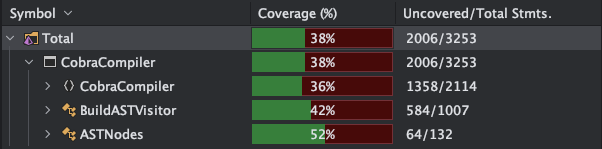
\includegraphics[width=0.8\textwidth]{Files/Billeder: Test/code_coverage.png}
    \end{center}
    \caption{Code coverage}
    \label{fig:code_coverage}
\end{figure}

\section{Unit Test}
The first level of testing conducted is unit testing. Unit testing is the smallest testable part of an application and the purpose of unit testing is to separate modules from their dependencies and test individual methods. The framework we use for testing is NUnit \cite{nunit}, which is a unit-testing framework for all .Net languages that support the AAA testing pattern. As mentioned in section \ref{sec:test_strat}, only some code is unit tested. This is due to most of the \lang compiler consisting of visitor patterns which are easier to test using integration testing because of the number of functions integrated with each other. This is shown in section \ref{sec:intergationTest}.\\

An example of a unit test can be seen in listing \ref{list:symbol_newscope_pushtostack}. The function being tested is \textit{NewScope()} by asserting if a new scope had been added to the stack of scopes in the symbol table. The Arrange block creates new instances of \textit{SymbolTable()} and \textit{BlockNode()} on lines 57-58. In the Act stage, \textit{NewScope()} in the symbol table is called and the block node is passed as an argument to the method. This happens on line 61. This should open a new scope containing the given block node. To test that \textit{NewScope()} did push this new scope to the stack, we test that our \textit{symbolTable.\_stackScopes} contains one scope on line 64. This will return true if \textit{NewScope()} pushes a new scope onto the stack. We also test that the stack contains a scope with a block that is equal to \textit{blockNode} on line 65. When running these tests, a green mark is displayed if all of the Assert methods return true. If this is the case, it can be concluded that these unit tests are successful, and in this case, the \textit{NewScope()} method in listing \ref{list:symbol_newscope_pushtostack} works as expected.

\begin{lstlisting}[language = csharp, firstnumber=53, label={list:symbol_newscope_pushtostack}, caption=Unit test of the NewScope() method that creates a new scope and tests if it pushes this scope to the stack - PEAKCompilerTesting / SymbolTableUnitTest.cs]
[Test]
public void NewScope_PushesScopeToStackScopes()
{
    // Arrange
    var symbolTable = new SymbolTable(new ErrorHandler());
    var blockNode = new ASTNodes.BlockNode();

    // Act
    symbolTable.NewScope(blockNode);

    // Assert
    That(symbolTable._stackScopes, Has.Count.EqualTo(1));
    That(symbolTable._stackScopes.Peek().Block, Is.EqualTo(blockNode));
}
\end{lstlisting}

\section{Integration Test} \label{sec:intergationTest}
As unit testing is for verifying the individual performance of modules and methods, integration testing has the purpose of verifying that they still exhibit the expected behavior as a group. This means that individual modules are combined and tested as a group to evaluate the compliance of the compiler. This section will test how the lexer, parser, AST builder, code generator, and so on work in conjunction.\\

The code in listing \ref{list:symbol_lookup_unittest} is the integration test for \textit{lookup()} in the symbol table. The \textit{SymbolTableintegrationTest} class contains all integration tests associated with the symbol table. The integration test in listing \ref{list:symbol_lookup_unittest} starts by creating a new instance of the \textit{SymbolTable} on line 9. Then a \textit{BlockNode} named \textit{blockNode1} gets instantiated on line 10. Then \textit{NewScope()} in the symbol table is called with \textit{blockNode1} as its argument on line 11. The \textit{Insert()} method is called twice to insert \textit{"x"} and \textit{"y"} in the current scope, which is the one belonging to \textit{blockNode1}. This happens on line 12-13. This concludes the Arrange stage. In the Act stage, we call \textit{Lookup()} in the symbol table three times on line 16-18. This looks for \textit{"x"}, \textit{"y"}, and \textit{"z"} in the current scope. These methods return objects of type \textit{Symbol} which contains a name, reference, and type. These symbols are checked in the assert section to see if the names of the symbols match what is expected. \textit{"z"} is not inserted in the symbol table and should therefore return \textit{null}. These asserts happen on line 21-23.\\

\begin{lstlisting}[language = csharp, firstnumber=3, label={list:symbol_lookup_unittest}, caption=Integration test of the lookup method from the symbol table - PEAKCompilerTesting / SymbolTableIntegrationTest.cs]
public class SymbolTableIntegrationTest
{
    [Test]
    public void Lookup_ReturnsCorrectSymbol()
    {
        // Arrange
        var symbolTable = new SymbolTable(new ErrorHandler());
        var blockNode1 = new ASTNodes.BlockNode();
        symbolTable.NewScope(blockNode1);
        symbolTable.Insert("x", ASTNodes.TypeEnum.text, blockNode1);
        symbolTable.Insert("y", ASTNodes.TypeEnum.text, blockNode1);
        
        // Act
        var result1 = symbolTable.Lookup("x", blockNode1);
        var result2 = symbolTable.Lookup("y", blockNode1);
        var result3 = symbolTable.Lookup("z", blockNode1);

        // Assert
        Assert.That(result1.Name, Is.EqualTo("x"));
        Assert.That(result2.Name, Is.EqualTo("y"));
        Assert.That(result3, Is.Null);
    }
}
\end{lstlisting}

\noindent The second integration test shown in listing 
\ref{list:EmitterTest} is a visit function for visiting the program node in the code generation phase. Code generation is done by the \textit{Emitter} class, which goes through the program, using the visitor pattern, and converts the program into the equivalent version in C. The C version is kept in a string builder which can then be tested. A string of \lang code that is used for testing the emitter can be seen on line 85. The string declares a number variable \textit{x} to the value \textit{10}. All the phases that lead up to the code generation, are then run in the rest of the arrange section. In the Act section, the function which visits the root node in the emitter is run on line 89. The generated C code is returned to a variable \textit{sb} of type string builder. The expected string of C code is built on line 91-95, and are then tested for equivalence in the Assert section on line 98. The goal of this test is to make sure, the emitter returns the correct C program as a string.\\

\begin{lstlisting}[language = csharp, firstnumber=82, label={list:EmitterTest}, caption=Integration test of the Emitter class used in the code generation phase - PEAKCompilerTesting / EmitterTest.cs]
public void EmitterVarDec()
{
    // Arrange
    var exprText = "number x = 10;";
    ...
    
    // Act
    StringBuilder sb = new Emitter(st).Visit((ASTNodes.ProgramNode)ast);

    String testString = "#include <stdio.h>\n#include <stdlib.h>\n#include <string.h>\nchar* concat(const char *str1, const char *str2) " 
        + 
        ...
        +
    "return curr_node->value;\n}\nvoid main(){\nint x = 10;\n}\n";

    // Assert
    Assert.That(sb.ToString(), Is.EqualTo(testString));
}
\end{lstlisting}

\section{Acceptance Test} \label{AccTest}
This section will cover the acceptance tests made to determine if the \lang compiler generates the correct target code. This is done by running a number of \lang code examples through our compiler and checking whether the resulting programs are as expected. These tests are based on the beginner exercises explained in section \ref{requirements}. If the code compiles correctly to C without errors, the C code is then compiled and run in order to see if the terminal prints the expected results. Furthermore, the generated C program is inspected to ensure it is correctly translated.\\ 
Each test contains the code written in \lang, then the code compiled to C, and finally the result of compiling and executing the C code.

%\cite{miller2001acceptance}

\subsection{Code Example: Scope test} \label{test_scopee}
The code example in listing \ref{list:acceptance_test_scope} is used to show that the scope rules defined in chapter \ref{ch:language_design} work as intended in \lang. In the example, a number \textit{y} is declared in the outer scope on line 1 with the value \textit{10}. Then \textit{print()} is declared which prints \textit{y} using \textit{output()} on line 2-5. \textit{output()} is then called with \textit{y} in the outer scope on line 6. In the if statement with condition \textit{true}, \textit{print()} is called followed by \textit{y} being outputted on lines 7-10. Then \textit{y} is redeclared with value \textit{12} on line 11 and then \textit{print()} is called, followed by \textit{y} being outputted on line 12-13. The \textit{print()} functions declaration can only access the global \textit{y} with value \textit{10} and should therefore output \textit{10},  while the \textit{output()} on line 13 should print \textit{12}. After the if-statement the \textit{print()} and \textit{output()} functions should output \textit{10} on line 15-16. The result can be seen in figure \ref{figure:scope_result}.

\newpage
\subsubsection{Source Code in \lang:}
\begin{lstlisting}[language = scriptkid, firstnumber=1, label={list:acceptance_test_scope}, caption=Acceptance test scope code examples]
number y = 10; 
function print() return nothing 
{ 
    call output(y); 
} 
call output(y);
if(true) 
{	 
    call print(); 
    call output(y);
    number y = 12; 
    call print(); 
    call output(y);
}
call print();
call output(y);
\end{lstlisting}

\subsubsection{Target code in C:}
In listing \ref{list:acceptance_test_scope_output}, the generated C code from the scope test program is displayed. From lines 1-4, the void function \textit{print()} is defined. It takes a parameter \textit{y}, which is then outputted in the function. \\
When first creating this test, an issue arose which was caused by translating the scope rules defined in \lang's semantics to code written in C. This issue was caused by the differences in starting points for \lang and C. In both C and \lang, functions can only be declared in the global scope. However, unlike in \lang where the starting point is placed at the first line of code, C uses the function \textit{main()} as its starting point. This results in a problem when declaring functions in \lang, which is addressed in section \ref{emitter:functions}. \\
The original version is identical to the output shown in listing \ref{list:acceptance_test_scope_output} except in the original, where nothing is used to distinguish between the first and second declarations of the variable \textit{y}. The \textit{print\_()} function on line 13 referenced the \textit{y} variable initialized on line 12, but in reality, it should have referenced the \textit{y} on line 6.\\
This issue required a fix to help distinguish between declared variables of the same name. The fix is described in section \ref{Implementation:SymbolTableScopeFix}. The code snippet shown in listing \ref{list:acceptance_test_scope_output} displays the resulting C code after the fix, and correlates with the program in \lang. The result when executing the code can be seen in figure \ref{figure:scope_result}.

\newpage
\begin{lstlisting}[language = C, captionpos=b, firstnumber=1, label={list:acceptance_test_scope_output}, caption=Acceptance test scope code examples in C]
void print_(int y)
{
    printf("%d\n", y);
}
void main() {
    int y = 10;
    printf("%d\n", y);
    if (1)
    {
        print_(y);
        printf("%d\n", y);
        int y_ = 12;
        print_(y);
        printf("%d\n", y_);
    }
    print_(y);
    printf("%d\n", y);
}
\end{lstlisting}

\subsubsection{Result:}
\begin{figure}[H] 
    \begin{center}
        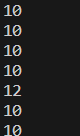
\includegraphics[width=0.20\textwidth]{Files/Billeder: Appendix/Scopetest.png}
    \end{center}
    \caption{The result for the scope code example}
    \label{figure:scope_result}
\end{figure}

\newpage
\subsection{Code Example: Update of variables} \label{test_UpdateVar}

The code example in listing \ref{list:acceptance_test_input_update_test} is used to show that declaration and re-assignment of an existing variable works as intended. First, multiple different variables of different types are declared on lines 1-3, and \textit{n} is then outputted on line 5. Afterward, the user is prompted for a new input for \textit{n} on line 7. This new value of \textit{n} is then outputted on line 9. A couple of examples of comments can be seen on lines 10-11, which are ignored when compiling to C. The new \textit{n} should overwrite the original value of \textit{n}.

\subsubsection{Source Code in \lang:} \label{}
\begin{lstlisting}[language = scriptkid, firstnumber=1, label={list:acceptance_test_input_update_test}, caption=Acceptance test update of variables with input code examples]
number n = 123;
text t = "test";  
decimal d = 0.20123123947342375;  
call output("Previous value is "); 
call output (n); 
call output(". Please input a new number");
n = call number input();  
call output("New value is "); 
call output(n);  
comment: This is a comment;
comment: This is also a comment;  
\end{lstlisting}

The C code in listing \ref{list:acceptance_test_input_update_text_output} corresponds to what is expected. First, the three different variables are declared on lines 3-5, whereafter three lines are printed to the console on lines 6-8. Next, \textit{input()} is called. The input function is a custom helper function that is added to the emitter. It takes in a format and the variable size, scans a user input, and returns it. The \textit{input()} function returns a void pointer, which needs to be cast to the correct pointer type and dereferenced to get the value. This can be seen on line 9. Note that the decimal value in listing \ref{list:acceptance_test_input_update_test} is rounded up when compiling to C. This is because float only being able to contain 7 decimals \cite{Float7Dec}. This was first discovered when running the code example in listing \ref{list:acceptance_test_input_update_text_output}. This is touched upon in the discussion section \ref{Diss:CompilerRev}. The result when executing the code is displayed in figure \ref{figure:input_update_result}.

\subsubsection{Target code in C:}
\begin{lstlisting}[language = C, firstnumber=1, captionpos=b, label={list:acceptance_test_input_update_text_output}, caption=Acceptance test update of variables with input code examples in C]
void main()
{
int n = 123;
char * t = "test";
float d = 0.20123124;
printf("%s\n", "Previous value is ");
printf("%d\n", n);
printf("%s\n", ". Please input a new number");
n = *(int *)input("%d", sizeof(int));
printf("%s\n", "New value is ");
printf("%d\n", n);
}
\end{lstlisting}

\subsubsection{Result:}
\begin{figure}[H] 
    \begin{center}
        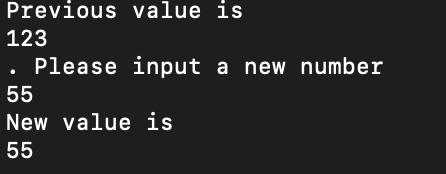
\includegraphics[width=0.40\textwidth]{Files/Billeder: Appendix/InputUpdate.png}
    \end{center}
    \caption{The result for the variable update code example}
    \label{figure:input_update_result}
\end{figure}

Along with these examples, some other acceptance tests are also made. These can be seen in section \ref{Appendix:acceptance_test} in the appendix. A short description of these examples can be seen below:

\begin{itemize}
    \item \textbf{Insertion-Sort:} This code example initializes a list of numbers and prints them. Afterward, this list is sorted using the 'SortNumberList()' which uses the insertion-sort algorithm. The new sorted list is then also printed.
    \item \textbf{Time-Conversion:} This code takes a number of seconds as input. By using division and a function 'mod()', which calculates modulo, it calculates how many weeks, days, hours, and minutes these seconds are equivalent to. These values are then printed.
    \item \textbf{GCD calculator:} This code calculates the 'greatest-common-divisor' of two numbers. this code includes 'GetMax()', 'GetMin()' and 'mod()'. In case the given input is wrong, the user is asked once again for an input. After printing GCD, the code gives the user the opportunity to write two new numbers.
    \item \textbf{Input Repeat:} This example declares a function called 'StartFunction()'. This function has a while-loop which runs while a boolean value is true. In the loop, the user is prompted and asked to write "start" to begin. The user is then asked to write how many times a message should be repeated. A message saying "This is a repeated message" is then repeated to the number requested by the user. Afterward, the user is prompted to write 'start' again.
    \item \textbf{Triangle Area:} This example declares a function 'triArea()' which calculates the area of a triangle. This function is then called and printed four times, all with different inputs.
    \item \textbf{Mathematical Expressions:} This example tests that all the mathematical expressions included in \lang works as intended. This is done by declaring variables and using the infix mathematical expressions on the variables.
    \item \textbf{Missing semi error:} This code example is used to test if the correct error is being output when the code is missing a ";".
    \item \textbf{Wrong type:} This code example tests the output message for when an incorrect type has been used.
    \item \textbf{String concatenation:} This code example is used to test for string concatenation. this is done by creating a text variable and using the infix operator "+" between two strings, and afterward outputting the variable.
    \item \textbf{Zero division:} This code example is used to make sure that division by zero is not possible in \lang and that it gives the correct output in the terminal.
\end{itemize}

\subsection{User Testing}\label{usertesting}
In order to test and get feedback on whether or not \lang has succeeded to become a beginner-friendly programming language, a user testing plan is produced.
First up, the tester has to be exposed to a number of small programs written in two different languages, one should be \lang and the other should be in a non-beginner-friendly language as mentioned in section \ref{SelectionLang}. The purpose of this is to test the readability of \lang, by having the tester look through these programs and write down what the tester thinks the programs do.\\


%The last part of the user test will cover the usage of \lang. The tester have to be introduced to \lang functionality, and the basics of it, and then write a specific program. Afterward, you could then show the tester another language and ask them to write the same program in that language. That way, we could see whether or not \lang is more intuitive to learn syntax-wise than a language for more experienced programmers. This type of test would suit more experienced beginner programmers than a beginner program that has not programmed before, as you would need the basic foundation of how to program.\\

Second, the user test will cover the usage of \lang. The tester has to be introduced to \lang functionality, and the basics of it, to be able to write a basic beginner programming exercise, like those explained in section \ref{requirements}, that the requirement for \lang is build upon. In this test, we will observe if the tester has problems writing code in \lang. This is done to test whether or not it is intuitive to learn and use the syntax. It has not been possible to get a user test conducted. This is due to lack of time, discussed in section \ref{discussion:Time}. 

%Furthermore, it would be beneficial if the tester is introduced to another language too, and write the same program, to compare the performance. This type of test would however require the beginner programmers to have the basic foundation of how to program.\\
%By going through user testing for \lang, a beginner programmer could give us feedback on whether or not our language is suited for beginner programmers. As well as comparing the learning progress of using \lang and another text-based industry language. 
\chapter{Discussion}
This chapter will discuss the development of the \lang compiler, as well as reflect on the extent to which \lang meets the requirements. 

\section{Language Revisions}
The goal with \lang's syntax is to balance the readable concepts from block-based languages, with the industry standards. The three criteria we followed in regard to designing a programming language were as described in section \ref{languageCriteriaForLang}: Readability, Writability, and Reliability.

\subsubsection{Readability:}
Based on the analysis, it was decided that \lang should have high readability because new concepts are harder to understand for beginners. After reflection, it can be asserted that this goal was met with \lang because the syntax described in the Syntax Design section \ref{sec:SyntaxDesign}, is arguably highly readable because it is closely related to natural language. This is highlighted in table \ref{tab:peaklanguageCriteria}, where simplicity, Data Types, and Syntax design all are check-marked, under the readability column.\\

However, it could be argued that some parts of \lang could be more readable. Because the goal for \lang is to become a language for transitioning to industry standard languages, some of the syntax is less readable.\\
Taking the list helper function into consideration, the "\textit{list}:add(\textit{x})" is more readable and related to the English language if it is instead written as: "add \textit{x} to \textit{list}". Another example of less readable syntax is the use of curly brackets to define scopes in \lang. Alternatively, a more readable approach would have been to use "begin" and "end", like used in Quroum. However, our own experience when learning to program was that using curly brackets for defining scopes, was not difficult to understand. Most popular programming language (except Python) uses curly brackets \cite{TopProgrammingLanguages2022}, and therefore curly brackets were included in \lang. 


\subsubsection{Writability:} 
The aim for \lang was to have fairly low writability, as high writability is often associated with shorter syntax and faster-to-write features, which can lead to confusion for beginners. This goal was arguably met, as much of the syntax in \lang was not compromised in terms of simplifying certain features. An example of this is the implementation of function declarations seen in semantic definition \ref{funcDec_BS}, where keywords such as \textit{function} and \textit{return} are used, in order to increase readability, but compromise writability. In the criteria table \ref{tab:peaklanguageCriteria} below, the lack of writability is shown in the majority of crosses under the writability column. 

 \subsubsection{Reliability} We wanted high reliability in \lang because a clear understanding of what is happening when programming will help beginner programmers develop. In order to achieve this, complex concepts such as pointers and exception handling, are excluded from \lang. Additionally \lang uses a static type binding, which promotes scope rule understanding. In general, these features were implemented as set out. Table \ref{tab:peaklanguageCriteria} highlights that reliability was significant under multiple categories, as seen by the checkmarks shown under Type Checking, Restricted Aliasing, Simplicity, etc.

Based on these reflections the following criteria table \ref{tab:peaklanguageCriteria} was created, which highlights how \lang turned out in terms of the different criteria. The table was created based on how the \lang turned out. A checkmark (\checkmark) means \lang expresses a high significance within that category, and a cross (X) means that \lang lacks implementation or priority within that category.

\begin{table}[H]
\centering
\resizebox{0.75\textwidth}{!}{%
\begin{tabular}{l|lll}
                    & Readability               & Writability & Reliability               \\ \hline
Simplicity              & \checkmark & \checkmark & \checkmark \\
Orthogonality       & X                         & X           & X                         \\
Data Types          & \checkmark & X           & \checkmark \\
Syntax Design       & \checkmark & X           & \checkmark \\
Support for Abstraction &                           & \checkmark & \checkmark \\
Expressivity        &                           & X          & X                         \\
Type Checking       &                           &             & \checkmark \\
Exception Handling  &                           &             & X                         \\
Restricted Aliasing &                           &             & \checkmark
\end{tabular}%
}
\caption{Language Criteria for PEAK+}
\label{tab:peaklanguageCriteria}
\end{table}

Throughout the process, \lang went through two iterations. The first iteration was much simpler, but still took the majority of the time, simply because there was a learning curve to developing a compiler. Once the first iteration was finished, a template existed for implementing many of the additional features that were needed to meet the requirements set out in table \ref{tab:requirements}.

\subsection{Compiler revisions} \label{Diss:CompilerRev}
\subsubsection{Compiler Language}
The first iteration compiled to C\# as the target code. This was because initially we had more experience with C\#, but through the process, it became more clear that C was a better language to target. This was realized with instances such as the static binding rules in C, as well as the general flexibility. Therefore the second iteration was developed with C as the target language. With these reflections in mind, the following subsection will describe in detail to what extent the requirements of \lang have been met. \\

\subsubsection{Decorated AST}
In section \ref{peakCompiler} of the implementation chapter, it was stated that the \lang compiler did not ever decorate the AST. When testing string concatenation in the emitter, this needed to change because of an issue. Adding two \textit{text} values in an addition node has to be handled differently than adding numbers in the emitter. Therefore infix-expression nodes in the AST needed to store the type to which the node evaluates to, resulting in the AST being decorated. This happens in the type checker. 

\subsubsection{Decimal to float}
During testing, we discovered, that values of type \textit{decimal} with many decimal numbers, would be rounded down to 7 decimals in the target code. This is because when trying to store a \textit{decimal} value in \lang in the AST, it gets stored as a float, which automatically is rounded up to 7 decimals. Alternatively, it could have been stored as a double instead. Float was chosen as \lang is not designed for creating large precise calculations. However, choosing double could have increased \lang's reliability as it might not be clear to the user that the \textit{decimal} value is rounded up.\\

\newpage
\section{Requirement evaluation} % Eventuelt tilføje en requirement fulfillment table som vi lavede i P3 s. 97
All requirements in table \ref{tab:requirements} will be evaluated in order to assess whether \lang has successfully achieved all of the desired requirements. 

\subsubsection{Must have requirements evaluation}
In this section, all the must-have requirements from table \ref{tab:requirements} will be assessed in order to evaluate if they have been fulfilled and that \lang has all the features deemed essential.
\begin{itemize}
    \item M1 - Declaration and assignment of number, decimal, text, and boolean variables.
\end{itemize}
The must-have requirement \textit{M1} has been fulfilled by making it possible to declare and assign variables of the types: \textit{number}, \textit{decimal}, \textit{text}, and \textit{boolean}. An example of this can be seen in the code example section \ref{test_UpdateVar}. In this code example, a \textit{number}, \textit{text}, and \textit{decimal} variable are declared and give the correct output. For this reason requirement \textit{M1} has been fulfilled.
\\
\begin{itemize}
    \item M2 - Display output and take keyboard input in the console.
\end{itemize}
This must-have requirement states that \lang should be able to display output in the console and receive inputs. This has been done by creating the \textit{"call output()"} and \textit{"call input()"} methods. An example of this can be seen in listing \ref{list:acceptance_test_input_update_test} which shows that both input and output works as intended. Because of this the must-have requirement \textit{M2} has been fulfilled
\\
\begin{itemize}
    \item M3 - Basic iterative and selective control structures
\end{itemize}
This must-have requirement says that \lang should contain both iterative and selective control structures. The iterative control structures was added through the implementation of a while loop and for loop. An example of this can be seen in the appendix chapter in section \ref{acc_test_Seconds}. The selective control structure has been implemented by the use of if-else statement. An example of an if-else statement can also be seen in the appendix chapter in section \ref{acc_test_Calcc}. Because \lang has both iterative and selective control structures the \textit{M3} requirement has been fulfilled.\\


\begin{itemize}
    \item M4 - Basic arithmetic \& logical operations.
\end{itemize}
This must-have requirement requires \lang to include basic mathematical operations. This is done by implementing the infix operators "+, -, *, /" and parenthesis operators "(" and ")" , and the logical operators "<, >, <=, >=, and, or, is, is not" (as mentioned in section \ref{OrderPrec}. An example program of mathematical operations can be seen in the appendix chapter \ref{Appendix:acceptance_test} in figure \ref{test_MathExpr}. In this code example all the mathematical operations have been implemented. This can be seen in the result of figure \ref{test_MathExpr}. For this reason, the \textit{M3} must-have requirement has been fulfilled.
\\
\begin{itemize}
    \item M5 - Syntax which resembles concepts and terminology used in
high school education.
\end{itemize}
As mentioned in table \ref{tab:requirements}, the syntax has to resemble concepts and terminology used in high school, for example the use of fully spelled words and basic math symbols. This can be seen in the code examples in section \ref{AccTest} and the appendix chapter \ref{Appendix:acceptance_test}. \lang uses fully spelled words as \textit{number} or \textit{text}. By doing this the must-have requirement has been fulfilled.
\\
\begin{itemize}
    \item M6 - Error messages at compile time.
\end{itemize}
This must-have requirement states that \lang must have error messages at compile time. This has been done by outputting error-messages in the terminal during compilation. An example of this can be seen in the appendix chapter \ref{Appendix:acceptance_test} in figure \ref{test_MissingSemi}, where an error message is being displayed in the terminal due to a missing semicolon. Another example can also be seen in the appendix chapter \ref{Appendix:acceptance_test} in the figure \ref{test_TypeErr}, displaying a type error, due to the type being \textit{text}, but the value is of type \textit{number}. Because of this the must-have requirement \textit{M5} has been fulfilled.

\subsubsection{Should have requirement evaluation}
In this section, all the should-have requirements from table \ref{tab:requirements} will be evaluated.
\begin{itemize}
    \item S1 - A for each loop.
\end{itemize}
This requirement states that \lang should contain a way to create a for each loop similar to the one used in a language like C\#. In \lang, this has been done by using the keyword \textit{repeat} followed by \textit{for each}. The way it was implemented in C can be seen in the implementation chapter in section \ref{for each impl}. An example of a for each loop in \lang can be seen in the appendix chapter \ref{Appendix:acceptance_test} in figure \ref{test_insertion}. By implementing the \textit{for each} loop in \lang, the should-have requirement \textit{S1} has been fulfilled.
\\
\begin{itemize}
    \item S2 - String concatenation.
\end{itemize}
This requirement states that \lang should contain the possibility to do string concatenation. An example of how string concatenation has been achieved in \lang can be seen in the appendix chapter \ref{Appendix:acceptance_test} in figure \ref{test_stringconc}. By being able to do string concatenation, the \textit{S2} requirement has been fulfilled.
\\
\begin{itemize}
    \item S3 - Declaration and assignment of lists
\end{itemize}
To complete this should-have requirement \lang should have the feature of declaring and assigning lists. The way the declaration and assignments of lists have been implemented can be seen in the implementation chapter \ref{ch:implementation} in section \ref{implement list}. Some code examples for declaring and assigning lists can be seen in the appendix chapter \ref{Appendix:acceptance_test} in figure \ref{test_insertion}. As can be seen in the figure, by being able to declare and add values to a list, the should-have requirement \textit{S3} has been fulfilled.
\\
\begin{itemize}
    \item S4 - List helper functions like add and remove from the lists.
\end{itemize}
To complete the should-have requirement \textit{S4}, list helper functions like \textit{Add()} or \textit{Remove()} should be added. Like the should-have requirement \textit{S3}, the implementation for this can be seen in the implementation chapter \ref{ch:implementation} in section \ref{implement list}. In figure \ref{test_insertion} in the appendix chapter \ref{Appendix:acceptance_test}, it is possible to see the helper function \textit{Add()} in the code example. Under development, it was decided to replace the \textit{Remove()} helper function with a \textit{Replace()} instead and add the \textit{ValueOf()} and \textit{IndexOf()} operators. The reason for not including a \textit{Remove()} operator was because of the difficulty of deleting an element in the middle of a list. This is because in \lang no value for null exists, so it was unclear what to do with a missing element, even though, a \textit{Remove()} operator is very intuitive and well-suited for a beginner programmer. By having the \textit{Add()}, \textit{Replace()}, \textit{ValueOf()}, and \textit{IndexOf()} list helper functions are implemented in \lang. However, since the \textit{Remove()} is not implemented the should-have requirement \textit{S4} has not been fully completed.
\\
\subsubsection{Could have requirement evaluation}
\begin{itemize}
    \item C1 - Support for abstraction in the form of methods
\end{itemize}
This could-have requirement states that \lang could include the feature of being able to create methods. The implementation of methods can be seen in the implementation chapter \ref{ch:implementation} in section \ref{emitter:functions}. An example of a method being created in \lang can be seen in figure \ref{test_scopee} in the acceptance test chapter \ref{AccTest}. For this reason the could-have requirement \textit{C1} has been fulfilled.
\\
\\
\begin{table}[H]
\centering
% Please add the following required packages to your document preamble:
% \usepackage[table,xcdraw]{xcolor}
% If you use beamer only pass "xcolor=table" option, i.e. \documentclass[xcolor=table]{beamer}
\begin{tabular}{|l|llllll}
\cline{1-1}
\textbf{Requirements overview} &                                                 &  &  &  &  &  \\ \hline
\textbf{Must have} &
  \multicolumn{1}{l|}{\cellcolor[HTML]{32CB00}{\color[HTML]{333333} M1}} &
  \multicolumn{1}{l|}{\cellcolor[HTML]{32CB00}M2} &
  \multicolumn{1}{l|}{\cellcolor[HTML]{32CB00}M3} &
  \multicolumn{1}{l|}{\cellcolor[HTML]{32CB00}M4} &
  \multicolumn{1}{l|}{\cellcolor[HTML]{32CB00}M5} &
  \multicolumn{1}{l|}{\cellcolor[HTML]{32CB00}M6} \\ \hline
\textbf{Should have} &
  \multicolumn{1}{l|}{\cellcolor[HTML]{32CB00}S1} &
  \multicolumn{1}{l|}{\cellcolor[HTML]{32CB00}S2} &
  \multicolumn{1}{l|}{\cellcolor[HTML]{32CB00}S3} &
  \multicolumn{1}{l|}{\cellcolor[HTML]{FFFF00}S4} &
   &
   \\ \cline{1-5}
\textbf{Could have}            & \multicolumn{1}{l|}{\cellcolor[HTML]{32CB00}C1} &  &  &  &  &  \\ \cline{1-2}

\end{tabular}
\caption{An overview of each individual requirement.}
\label{tab:reqfulfillmentoverview}
\end{table}
\noindent
Through this requirement evaluation all must-have, should-have \& could-have requirements have been evaluated as well as fulfilled, except for the S4 requirement. By having most requirements fulfilled in the above-mentioned requirements it is deemed that \lang has the most essential features implemented and usable in the language.
\\

However, it is important to consider the development of these requirements was based on the problem analysis. Even though our own experiences also have been taken into consideration, as experienced programmers, we have a bias towards what we believe to be hard and easy concepts to understand in programming. This could result in us having created a language that is not actually beginner-friendly, as our understanding of a beginner-friendly language may differ from an actual beginner's perspective on what they find more educational. Because of this, it can be argued that we have no confirmation on the claim that \lang is a good tool for beginner programmers to learn to code. Therefore user testing would be fairly wanted, however, this was not conducted due to time loss, as touched upon in section \ref{usertesting} and \ref{futurework:Usertesting}.

\section{Time Management} \label{discussion:Time}
%Hvorfor var det lige at vi blev forsinket med testing pga. 2. code generation - forklar her hvorfor vi ikke nåede alt det vi skulle mht til testing osv. Lang tid på ANTLR, lang tid på CodeGen fejl.  Generelt svært at planlægge når alt i dette projekt var ny viden.  
%Måske noget med valg af parser? ANTLR var hurtig at starte, men langsom at fuldføre. Betød det noget for vores compiler at vi bruger LL og ikke LR?
One of the first decisions that we made was to use ANTLR for scanning and parsing the initial program. ANTLR's intuitive introduction and graphical interface caught our eye and seemed to be the best tool for first-time compiler developers. However, ANTLR turned out to be more difficult than expected to get used to and time consuming. In general, we needed to weigh the options on whether it was more worth to develop the parser ourselves or use a tool. In both scenarios, there was a learning curve with the process. \\

The decision to use ANTLR also led to the need of converting our CFG to LL(k) grammar. Ultimately the LL(k) parsing approach is less powerful than an LR(K) approach, however, it was easier to design the grammar so that it met the requirements for LL(k), which saved us time. \\

We decided to use an iterative model for the development of the compiler, and it was split into 2 iterations. Overall it was a good decision since it led us to a much stronger language. It was also a very natural decision in the context of developing a compiler since a compiler has concrete phases that all need to be updated to handle new feature or fixes. However, the 2nd iteration did take more time than we initially wanted, which led to some shortcomings that we had to be aware of. Mainly it was the testing of the compiler, which had to be pushed back. This inevitably led us to have a less complete testing section than we would have wanted, meaning not everything in the compiler ended up being tested. It would have been smarter to leave out some less important features of the language, which delayed the completion time of the 2nd iteration. In general, it was hard to plan ahead in detailed time increments, because of how new everything within this project was.

\section{Tests}
Testing was done after the compiler was finished with the 2nd iteration, which is not the most effective testing strategy. Optimally we would have used a Test-driven development (TDD) design process in order to be able to more definitively ensure that the code written was correct, and also in order to be able to test that the changes made to the existing constructs would not break existing functionality \cite{TDD}. Testing this way would give defined parameters to develop within, which potentially could have saved time. However, this idea of writing tests first is hard to do, because it requires a more structured approach, which can be difficult when developing a compiler for the first time. If tests were written beforehand, they would likely have taken just as long, if not longer to accurately write, and there is a good chance they would have had to be rewritten as the process moved along.

%Unit testing was a smaller part of testing than expected because most parts of the compiler were heavily integrated with each other, and there were only a few individual units that could be tested by themselves. Most of the unit tests were done on the symbol table, as it contained methods that were separate from the rest of the compiler. Instead, most of the remaining testing was done through integration testing.
%As seen in figure \ref{fig:code_coverage} the code coverage of tests reflects a time management issue, that resulted in us not being able to completely test all the code. Therefore, a few cases were covered per phase of the compiler, in order to argue that to a smaller extent, all phases of the compiler were tested. Much of the reason why testing could not be covered fully, was because multiple visitor patterns for different phases of the compiler contain over a thousand lines of code each, which gets expanded the more features are implemented in the language, meaning there simply was too much code to cover with the given time frame. \\

%Acceptance testing helped discover problems with the language, by writing small programs which tested the different constructs and their interactions after compilation. For example, during acceptance testing, problems were discovered, such as string concatenation not working as intended, functions using the wrong variables in specific cases, division by 0 being possible when it should not, etc. Hence, acceptance testing was a way of ensuring that the resulting code looked as expected after compilation and that the programs behaved as expected when running them. \\
% Decorated AST - to keep the type of strings to concatenation. 

\section{Future Work}
As this project is subject to deadlines, some aspects of the project will not be fulfilled to perfection. This section will cover the future works of this project, and what particular components could be added or worked on, to improve the overall result.

\subsection{User Test} \label{futurework:Usertesting}
A form of testing we did not get to cover was user testing. In order to better conclude that \lang was suitable for the set-out target audience, it would have been advantageous to let a group of beginner programmers, preferably high school students, test \lang. \\
Regarding which users to test on, first-semester software students of Aalborg University seemed evident. This is because these students are motivated to learn programming and have gone to high-school, as well as having just started to learn to code. The test that should be conducted is explained in \ref{usertesting}.\\
%The first tasks that should be tested in \lang by a user, should be simple programming tasks, such as those we encountered when we started on our first semester of software. This is because we ourselves found these tasks helpful in learning the basics of programming.\\

\subsection{Code Functionality}

%Functions in functions - not allowed.
%Helper functions ? (Basics to lists as length, slice so on) 
%- Comments ending with semicolon
%- Index strings
%- Typecasting
%- Structs
%- recursive functions
%- Concatenating a string with a number (In general, auto type conversion in specific cases)
%- Ability to copy lists (You have to create a loop in order to get the values of a list returned from a function into a list in your program. Otherwise you will only be able to use the list returned from the function at the point where you call the function and then it's lost after.)

While developing and testing the \lang compiler, some of the inconveniences with \lang were discovered, as well as missing features which were planned at first but were forgotten early on. These features made some of the programmer tasks we originally wanted beginner programmers to execute, impossible. This included:

\subsubsection{Indexing strings:}
While writing tests, an attempt of making a program that was able to detect whether a given string input was a palindrome was made. This programming task came from when we were learning to program ourselves in the "imperative programming" course \cite{C-CourseExercises}. This required a for-loop to go through the string and check whether a character in the front, matched a character at the end of the string. String indexing is often used in other languages like Python, C\#, or C and gives access to multiple ways of string manipulation. Alternatively, some of the list operations could have been made to also apply to \lang's \textit{text} type, like \textit{IndexOf()}.
    
\subsubsection{Built-in Operations:} In \lang, many components have to be built from the ground up. An example of this is getting the length of a list, which in \lang requires a for-each loop in order to iterate through the list and count the number of elements. For beginner programmers, this can seem tedious as many additional small functions are often needed in a program, which by default exist as constructs in other languages like C\#, python and C. Examples of built-in operations could be: \textit{number:Max()}, \textit{text:Length()}, \textit{list(text):Length()}, \textit{Decimal:Round()}. 

\subsubsection{Structs:} In order to teach the beginner programmer about object-like programming, structs were considered before making the first iteration. Structs would have made it possible for the beginner programmer to store values of certain types together. This would have made it possible for the beginner programmer to solve programming tasks such as creating a family tree, where each family member is of a "Person" struct. Alternatively, these kinds of tasks could be solved in \lang using multiple lists and indexes. For example a \textit{list(text) family} where [0] = "your name", [1] = "mom's name" and [2] = "dad's name" and a seperate list of \textit{list(boolean) isMale} where [0] = true, [1] = false.

\subsubsection{Typecasting:}
 The ability to typecast is also something that was discussed early on. This was one of the features which was only going to be added if any extra time was left. In \lang, you are not able to convert for example \textit{decimal} to \textit{numbers} or \textit{text} to \textit{numbers}. Being able to cast a string to an integer is often used in programming tasks. When learning about programming in the "imperative programming" course, we had a task, about calculating the overall scores of football teams. As input, a large text file about football scores was provided, which had to be converted to numbers in order to calculate the total scores \cite{C-CourseExercises}. In order to solve this task, typecasting would need to be available to the programmer. Alternatively, you can sometimes work around explicit typecasting in \lang. For example, by adding a \textit{number} together with "0.0", you would receive a \textit{decimal} value.

\subsubsection{Recursive functions:} Recursive functions were never discussed but are something that is often used in beginner tasks in order to teach the concept of recursion. Given more time, the recursive functions should be added to \lang, as it is an important concept in programming. The palindrome task mentioned earlier when talking about indexing strings also applies here. In the original task from the "imperative programming" course \cite{C-CourseExercises}, the goal was to solve this task first without using recursion, and then with, in order to see the difference.

\subsubsection{Arithmetic Operators:} Including a modulo arithmetic operator was never discussed and therefore forgotten. As modulo is an important tool in programming it should have been included, as the alternative is to create a \textit{mod()} function, calculating the modulo of two numbers. This is an extra step in \lang but is provided in other languages like C\#, C, and Python. An exponent operator using the symbol \^ was discussed shortly, as when the group recalled using math tools in high school, this way of creating exponents was natural for them. With this, the transition from high-school maths to programming would be smoother. 
\chapter{Conclusion}
% Konkluder ved hjælp af studieordningen og vores punkter under problem formuleringen.

%Start med at forklare projektet - Vi har lavet dette sprog som skla bruges af disse mennesker og som kan .. bum bum bum.. 
%Syntax, symantic osv. 

%rund af med at hvad intentionen var med sporget, og hvor virkeligheden så er endt. 
%Skal hænge sammen med abstract, (som indeholder hvad raporten indeholder..  fx. så mange typer og så mange test osv, vi har defineret en brugertest, men vi nåede de her tests.. 

This report details the development of \lang a programming language aimed towards introducing beginner programmers to text-based programming and some of the concepts of the industry standards, in an educational format. \lang has fundamental features, such as basic arithmetic, control structures, abstraction through functions, etc. with high readability. The challenge of designing \lang was a balancing act between using readable concepts from block-based languages, whilst still designing features that introduce users to the industry standards for programming languages. Based on this initial problem, the following problem statement was defined. 

\begin{center}
    \textit{How can a text-based programming language be developed for beginner programmers, using readable concepts from block-based languages, while focusing on facilitating the transition to programming languages used in the industry?}
\end{center} 

Based on the requirements described in the problem statement section \ref{problemstatement}, which aims towards creating a successful compiler for \lang, it can be concluded, that the parts and phases of a compiler that are required have been successfully implemented, tested and described. This includes but is not limited to the creation of a lexer, parser, AST design, correct scope rules, successful type checking, symbol table creation, code generation, testing as well as defining operational semantics for \lang. \\

Finally, It can be concluded that \lang has successfully met most requirements defined in section \ref{requirements} table \ref{tab:requirements}. Unfortunately, because of the lack of user testing, \lang's ability to serve as a beginner-friendly language cannot be entirely concluded as successful in a practical manner. Although the requirements are built upon the analysis, it is difficult to disregard the bias of an experienced programmer, compared to the mind of a beginner programmer. However, the analysis provides a blueprint of how \lang should be designed in order to cater to beginner programmers in high school. Hence it can be concluded that \lang has successfully fulfilled the problem statement.\\


%------------

% Based on the language requirements defined in table \ref{tab:requirements}, it can be concluded that the language has successfully met all the requirements, which were designed with the problem statement in mind.
% Unfortunately, because of the lack of user testing done on the language, its ability to serve as a beginner-friendly language cannot be entirely concluded as successful in a practical manner. However, the requirements are built upon Sebesta's language criteria. The analysis, therefore, provides a blueprint of how the language should be designed in order to cater to beginner programmers in high school. Hence it can be concluded that the language has successfully fulfilled the problem statement.In order to fully conclude whether the language has educational benefits, proper user testing should be done on the appropriate target audience. \\

% Finally, it can be concluded based on the requirements described in the problem statement section \ref{problemstatement}, which aim towards creating a successful compiler for \lang, that the parts and phases of a compiler that are required have been successfully implemented, tested and described. This includes but is not limited to a lexer, parser, AST design, correct scope rules, successful type checking, symbol table creation, code generation, testing as well as defining operational semantics for \lang. 


% \begin{itemize}
% %  \item Analyze beginner programmers.
%   \item Define language criteria.
% %  \item Explain the programming paradigm of \lang.
% %  \item Create a MoSCoW requirement table.
%   \item Create a Context-Free Grammar (CFG).
%   \item Define semantics.
%   \item Define the scope rules.
%   \item Design Abstract Syntax Tree (AST).
%   \item Create a lexer and parser.
%   \item Build symbol table and handle type checking.
%   \item Successful code generation
% %  \item Show how the Syntax analysis, the Contextual analysis, and the code generation have been implemented.
%   \item Testing of \lang, including unit testing, integration testing, and acceptance testing.
% %  \item Evidence in the form of tests, to support the claim that our language helps provide the beginner programmer with a better transition from our language to an industry-standard language.
% \end{itemize}
\printbibliography[heading=bibintoc]
\label{bib:mybiblio}
\appendix
\chapter{CFG} \label{chap:appa}
\begin{lstlisting}[language=scriptkid, label={list:BNFCFG},caption=Context-free grammar for \lang in BNF form]
Program -> Cmds   
Cmds -> Cmd Cmds | EPSILON   
Cmd -> Stmt | Dcl   
Dcl -> Type Id Ass ;   
Ass -> = Expr | EPSILON   
Stmt -> Id = Expr ; | CtrlStrct | ListStmt ; | FuncDef | FuncCall ; | CommentStmt ; | return Type ; 
Expr -> LogicOr OprOr   
OprOr -> or LogicOr OprOr | EPSILON   
LogicOr -> LogicAnd OprAnd   
OprAnd -> and LogicAnd OprAnd | EPSILON   
LogicAnd -> Equal OprEql   
OprEql -> is Equal OprEql | is not Equal OprEql | EPSILON   
Equal -> Bool OprBool   
OprBool -> > Bool OprBool | < Bool OprBool | >= Bool OprBool | <= Bool OprBool | EPSILON   
Bool -> Term OprExpr   
OprExpr -> + Term OprExpr | - Term OprExpr | EPSILON   
Term -> Factor OprTerm   
OprTerm -> * Factor OprTerm | / Factor OprTerm | EPSILON 
Factor -> ( Expr ) | FuncCall | ListOprExpr | Num | Decimal | String | Id | Boolean 
Block -> { Cmds } 
CommentStmt -> comment: StringChars 
CtrlStrct -> IfStmt | Loop   
IfStmt -> if ( Expr ) Block ElseIfStmt   
ElseIfStmt -> else if ( Expr ) Block ElseIfStmt | Else | EPSILON   
Else -> else Block   
Loop -> repeat Loops   
Loops -> LoopStmt | WhileStmt | ForeachStmt   
LoopStmt -> ( Expr ) times Block 
WhileStmt -> while ( Expr ) Block   
ForeachStmt -> for each ( Type Id in Id ) Block   
ListStmt -> ListOpr | ListOprExpr 
ListOpr -> Id : Add ( ArgList ) | Id : Replace ( ArgList ) 
ListOprExpr -> Id : IndexOf ( Expr ) | Id : ValueOf ( ArgList ) 
FuncCall -> call Id ( ArgList ) | call output ( ArgList ) | call Type input ( ArgList ) 
FuncDef -> function Id ( ParamList ) FuncReturn Block   
FuncReturn -> return FuncReturnType   
FuncReturnType -> Type | nothing   
ParamList -> Param ParamTail | EPSILON   
ParamTail -> , Param ParamTail | EPSILON   
Param -> Type Id   
ArgList -> Expr ArgTail | EPSILON   
ArgTail -> , Expr ArgTail | EPSILON   
Boolean -> true | false   
Type -> boolean | text | number | decimal | list ( Type )   
Id -> Letter Chars 
String -> '"' StringChars '"'  
StringChars -> StringChar StringChars | EPSILON 
StringChar -> Char | SpecialChar  
Chars -> Char Chars | EPSILON  
Char -> Digit | Letter   
Letters -> Letter Letters | EPSILON   
Letter -> a ... z | A ... Z | _   
Decimal -> Num . Num 
Num -> Digit Digits   
Digits -> Digit Digits | EPSILON   
Digit -> 0 ... 9 
SpecialChar -> ! | @ | # | £ | ¤ | $ | % | & | / | ( | ) | { | } | [ | ] | = | ? | + | - | ` | ^ | ~ | * | , | . | ~ | § | ½ 
\end{lstlisting}  


\chapter{ANTLR CFG + LEXER}
\begin{lstlisting}[language=scriptkid, label={list:ANTLRCFG},caption=Context-free grammar for \lang used in ANTLR]
    program: cmds;  
cmds: cmd cmds | /*epsilon*/;  
cmd: stmt | dcl;  
dcl: type ID ass SEMI;  
ass: ASSIGN expr | /*epsilon*/;   
stmt: ID ASSIGN expr SEMI |  
ctrlStrct |  
listStmt SEMI | 
funcDef | 
funcCall SEMI | 
commentStmt SEMI | 
RETURN type SEMI;   
expr: logicOr oprOr;  
oprOr: OR logicOr oprOr | /*epsilon*/;  
logicOr: logicAnd oprAnd;  
oprAnd: AND logicAnd oprAnd | /*epsilon*/;  
logicAnd: equal oprEql;  
oprEql: EQUAL equal oprEql | NOT equal oprEql | /*epsilon*/;  
equal: bool oprBool;  
oprBool: GREAT bool oprBool | LESS bool oprBool |   
GREATEQL bool oprBool| LESSEQL bool oprBool | /*epsilon*/;  
bool: term oprExpr;  
oprExpr: ADD term oprExpr | SUB term oprExpr | /*epsilon*/;  
term: factor oprTerm; 
oprTerm: MUL factor oprTerm | DIV factor oprTerm | /*epsilon*/;  
factor: LPAREN expr RPAREN | funcCall | listOprExpr | INT | DEC | STR | ID | boolean;  
block: LCURLY cmds RCURLY;  
commentStmt: COMM; 
ctrlStrct: ifStmt | loop; 
ifStmt: IF LPAREN expr RPAREN block elseIfStmt;  
elseIfStmt: ELSE IF LPAREN expr RPAREN block elseIfStmt | else |  
/*epsilon*/;  
else: ELSE block;   
loop: REPEAT loops; 
loops: loopStmt | whileStmt | foreachStmt; 
loopStmt: LPAREN expr RPAREN TIMES block; 
whileStmt: WHILE LPAREN expr RPAREN block; 
foreachStmt: FOREACH LPAREN type ID IN ID RPAREN block; 
listStmt: listOpr | listOprExpr; 
listOpr: ID COLON LISTADD LPAREN argList RPAREN |  
ID COLON LISTDEL LPAREN argList RPAREN; 
listOprExpr: ID COLON LISTIDXOF LPAREN argList RPAREN |  
ID COLON LISTVALOF LPAREN argList RPAREN; 
funcCall: CALL ID LPAREN argList RPAREN |  
CALL PRINT LPAREN argList RPAREN |  
CALL type SCAN LPAREN argList RPAREN; 
funcDef: FUNCTION ID LPAREN paramList RPAREN funcReturn block; 
funcReturn: RETURN funcReturnType; 
funcReturnType: type | NOTHING; 
paramList: param paramTail | /*epsilon*/; 
paramTail: COMMA param paramTail | /*epsilon*/; 
param: type ID; 
argList: expr argTail | /*epsilon*/; 
argTail: COMMA expr argTail | /*epsilon*/; 
boolean: TRUE | FALSE;  
type: BOOL | TEXT | NUM | LIST LPAREN type RPAREN | DECIMAL; 
\end{lstlisting}



\begin{lstlisting}[label={list:ANTLR LEXER},caption=Lexer for \lang used in the ANTLR CFG]
OR: 'or'; 
AND: 'and'; 
EQUAL: 'is'; 
NOT: 'is not'; 
GREAT: '>'; 
LESS: '<'; 
GREATEQL: '>='; 
LESSEQL: '<='; 

ASSIGN : '=' ; 
COMMA : ',' ; 
SEMI : ';' ;
COLON: ':';
LPAREN : '(' ; 
RPAREN : ')' ; 
LCURLY : '{' ; 
RCURLY : '}' ; 
TRUE: 'true'; 
FALSE: 'false';

ADD: '+'; 
SUB: '-'; 
MUL: '*'; 
DIV: '/'; 
BOOL: 'boolean'; 
TEXT: 'text'; 
NUM: 'number';
DECIMAL: 'decimal';
NOTHING: 'nothing';
LIST: 'list';
QUOTE: '"'; 
IF: 'if'; 
ELSE: 'else';
REPEAT: 'repeat';
TIMES: 'times';
WHILE: 'while';
FOREACH: 'for each';
IN: 'in';
FUNCTION: 'function';
RETURN: 'return';
CALL: 'call';
PRINT: 'output';
SCAN: 'input';
COMMENT: 'comment:';

LISTADD: 'Add';
LISTIDXOF: 'IndexOf';
LISTREPLACE: 'Replace';
LISTVALOF: 'ValueOf';

COMM: 'comment:'~(';')*;
STR: '"' (~'"')* '"';
DEC: ('+' | '-')? [0-9]+'.'[0-9]+; 
INT: ('+' | '-')? [0-9]+ ;
ID: [a-zA-Z_][a-zA-Z_0-9]* ; 
WS: [ \t\n\r\f]+ -> skip ; 
\end{lstlisting}

\chapter{Type System} \label{Appendix:TypeSystem}

This appendix acts as a continuation of the Type system defined in section \ref{sec:TypeRules} \\

\section{Expression} \label{Appendix:Typesystem:Eq}

\begin{equation}
    (NUMEXP_{TS}) \ E\vdash n: number
\end{equation}

\begin{equation}
    (DECEXP_{TS}) \ E\vdash d: decimal
\end{equation}

\begin{equation}
    (TEXTEXP_{TS}) \ E\vdash txt: text
\end{equation}

\begin{equation}
    (BOOLEXP1_{TS}) \ E\vdash \mathbb{T} : boolean
\end{equation}

\begin{equation}
    (BOOLEXP2_{TS}) \ E\vdash \mathbb{F} : boolean
\end{equation}

\begin{equation}
   (VAREXP_{TS}) \frac{E\ (x)\ =\ T}{\ E\ \vdash \ x\ :\ T}
\end{equation}

\begin{equation}
    (PAREXP_{TS}) \frac{\ e\ :\ B}{\ E\ \vdash \ (e)\ :\ B}
\end{equation}

\begin{equation}
   (LISTSEXP_{TS}) \frac{E\ \vdash\ e\ :\ B }
    {\ E\ \vdash \  list (B)\ :\ ok} 
    \ for \ e \in L
\end{equation}

\begin{equation}
    (DEC*1_{TS})\frac{E \ \vdash \ e_1 : \ decimal \ E \ \vdash \ e_2 : \ number \ }{E \ \vdash e_1 \star \ e_2 \ : \ decimal} \ \ \ \
    where \ \star \in \{ +, *, - , /\}
\end{equation}

\begin{equation}
    (DEC*2_{TS})\frac{E \ \vdash \ e_1 : \ number \ E \ \vdash \ e_2 : \ decimal \ }{E \ \vdash e_1 \star \ e_2 \ : \ decimal} \ \ \ \
    where \ \star \in \{ +, *, - , /\}
\end{equation}

\begin{equation}
    (NUMDIV_{TS})\frac{E \ \vdash \ e_1 : \ number \ E \ \vdash \ e_2 : \ number \ }{E \ \vdash e_1 / \ e_2 \ : \ decimal}
\end{equation}



\begin{equation}
    (BOOL*_{TS})\frac{E \ \vdash \ e_1 : \ boolean \ E \ \vdash \ e_2 : \ boolean \ }
    {E \ \vdash e_1 \star \ e_2 \ : \ boolean} \ \ \ \
    where \ \star \in \{ and, \ or, \ is, \ is \ not\}
\end{equation}

\begin{equation}
    (TXT_{TS})\frac{E \ \vdash \ e_1 : \ text \ E \ \vdash \ e_2 : \ text \ }{E \ \vdash e_1 + \ e_2 \ : \ text} \  
\end{equation}

\section{Statements}
\begin{equation}
(LISTSTM1_{TS}) \frac{E\ \vdash x\ :\ list(B) \ \ E\ \vdash\ (x_1,...,x_k)\ :\ B }
{\ E\ \vdash \ x:Add(x_1, ...,\ x_k)\ :\ ok}
\end{equation}
\begin{equation}
    (LISTSTM2_{TS}) \frac{E\ \vdash\ x\ :\ list(B) \ \ \ E\ \vdash\ x_1\ :\ B \ \ \ E\ \vdash\ n\ :\ number }
{\ E\ \vdash \ x:Insert(x_1,\ n)\ :\ ok}
\end{equation}
\begin{equation}
    (LISTSTM3_{TS}) \frac{E\ \vdash\ x\ :\ list(B) \ \  \ E\ \vdash\ n\ :\ number }
{\ E\ \vdash \ x:ValueOf(n)\ :\ B}
\end{equation}
\begin{equation}
(LISTSTM4_{TS}) \frac{E\ \vdash\ x\ :\ L  \ \  \ E\ \vdash\ e\ :\ B }
    {\ E\ \vdash \ x:IndexOf(e)\ :\ number}
\end{equation}

\begin{equation}
    (LISTSTM4_{TS}) \frac{E\ \vdash\ x\ :\ L \ \ \ E\ \vdash\ n\ :\ number }
{\ E\ \vdash \ x:Delete(n)\ :\ ok}
\end{equation}

\begin{equation}
    (IFSTM1_{TS}) \frac{E\ \vdash\ e\ :\ boolean \ \  \ E\ \vdash\ S\ :\ ok }
{\ E\ \vdash \ if(e)\ \lbrace S \rbrace\ :\ ok}
\end{equation}
\begin{equation}
    (IFSTM2_{TS}) \frac{E\ \vdash\ e\ :\ boolean \ \  \ E\ \vdash\ S_1, S_2\ :\ ok }
{\ E\ \vdash \ if(e)\ \lbrace S_1 \rbrace\ else \ \lbrace S_2 \rbrace:\ ok}
\end{equation}
\begin{equation}
    (REPEATSTM1_{TS}) \frac{E\ \vdash\ n\ :\ number \ \  \ E\ \vdash\ S\ :\ ok }
{\ E\ \vdash \ repeat\ (n)\ times \ \lbrace S \rbrace:\ ok}
\end{equation}
\begin{equation}
    (REPEATSTM2_{TS}) \frac{E\ \vdash\ e\ :\ boolean \ \  \ E\ \vdash\ S\ :\ ok }
{\ E\ \vdash \ repeat\ while\ (e) \ \lbrace S \rbrace:\ ok}
\end{equation}
\begin{equation}
    (REPEATSTM3_{TS}) \frac{E\ \vdash\ x_1\ :\ list(B) \ \ \ E\ \vdash\ x\ :\ B\ \ \  E\ \vdash\ S\ :\ ok }
{\ E\ \vdash \ repeat\ foreach\ (B\ x\ in\ x_1 ) \ \lbrace S \rbrace:\ ok}
\end{equation}
\begin{equation}
    (RETSTM1_{TS}) \frac{E\ \vdash\ f\ :\ (e_1 \ : \ T_1 \ , ... , \ e_k \ : \ T_k \ \mapsto \ T) \ \ \  E\ \vdash\ e\ :\ T }
{\ E\ \vdash \ return\ e\ :\ ok}
\end{equation}
\begin{equation}
    (RETSTM2_{TS}) \frac{E\ \vdash\ f\ :\ (e_1 \ : \ T_1 \ , ... , \ e_k \ : \ T_k \ \mapsto \ \varepsilon)}
{\ E\ \vdash \ return\ :\ ok}
\end{equation}


\chapter{Structural Operational Semantics} \label{appendix:SOS}

\subsubsection{Expressions}

\begin{equation}
    (NUM_{BS})\frac{n \rightarrow _{\textbf{Num}} v}{\sigma \circ Env_v \vdash n \rightarrow _{\textbf{Exp}} v}
\end{equation}

\begin{equation}
    (VAR_{BS})\frac{\sigma(Env_v(x)) = \ v}{\sigma \circ Env_v \vdash x \rightarrow _{\textbf{Exp}} v } \ \
        if \ Env_v[x \rightarrow l] \ and \ \sigma[l \rightarrow v]
\end{equation}

\begin{equation}
\begin{split}
    (\star_{BS})\frac{\sigma \circ Env_v\vdash e_1 \rightarrow _{\textbf{Exp}} v_1 \ \ \sigma \circ Env_v \vdash e_2 \rightarrow _{\textbf{Exp}} v_2 }{\sigma \circ Env_v \vdash e_1 \star e_2 \rightarrow \ _{\textbf{Exp}} \ v_1 \star v_2 } \\
    Where \ \star \in (*, -, >, \geq, \leq, <, and, or, is, is \ not)
\end{split}
\end{equation}

\begin{equation}
    \begin{split}
        (PLUSNUM_{BS})\frac{\sigma \circ Env_v\vdash e_1 \rightarrow _{\textbf{Exp}} v_1 
        \ \ \sigma \circ Env_v \vdash e_2 \rightarrow _{\textbf{Exp}} v_2 }
        {\sigma \circ Env_v \vdash e_1 + e_2 \rightarrow \ _{\textbf{Exp}} \ v_1 + v_2 } \\
        Where \ v_1, v_2 \in \mathbf{Num \cup Dec}
    \end{split}
\end{equation}

\begin{equation}
    \begin{split}
        (PLUSTXT_{BS})\frac{\sigma \circ Env_v\vdash e_1 \rightarrow _{\textbf{Exp}} v_1 
        \ \ \sigma \circ Env_v \vdash e_2 \rightarrow _{\textbf{Exp}} v_2 }
        {\sigma \circ Env_v \vdash e_1 + e_2 \rightarrow \ _{\textbf{Exp}} \ v_1v_2 } \\
        Where \ v_1, v_2 \in \textbf{Txt}
    \end{split}
\end{equation}

\begin{equation}
    \begin{split}
        (DIV_{BS})\frac{\sigma \circ Env_v\vdash e_1 \rightarrow _{\textbf{Exp}} v_1 
        \ \ \sigma \circ Env_v \vdash e_2 \rightarrow _{\textbf{Exp}} v_2 }
        {\sigma \circ Env_v \vdash e_1 / e_2 \rightarrow \ _{\textbf{Exp}} \ v_1 / v_2 } \\
        Where \ v_2 \neq 0
    \end{split}
\end{equation}

\begin{equation}
    (PAR_{BS})\frac{\sigma \circ Env_v\vdash e \rightarrow _{\textbf{Exp}} v}
    {\sigma \circ Env_v \vdash (e) \rightarrow \ _{\textbf{Exp}} \ v}
\end{equation}

\begin{equation}
\begin{split}
    (LISTVALUEOF_{BS})\frac{n \rightarrow _{\textbf{Num}} \ v_1 \ \ \  \sigma \ \circ \ Env_v \ \vdash \ x(v_1)\ = \ v_2}
    {\sigma \ \circ \ Env_v\ \vdash x:valueof(n) \ \rightarrow _{\textbf{Exp}} \ v_2} \\
    Where \ x(n) \ is \ a \ function \ that \ returns \ a \ value \ given \ the \ index \ of \ the \ list \ of \ x
\end{split}
\end{equation}

\begin{equation}
\begin{split}
    (LISTINDEXOF_{BS})\frac{\sigma \ \circ \ Env_v\ \vdash e \rightarrow _{\textbf{Exp}} \ v_1 \ \ \  \sigma \ \circ \ Env_v \ \vdash \ x(v_1)\ = \ v_2}
    {\sigma \ \circ \ Env_v\ \vdash x:indexof(e) \ \rightarrow _{\textbf{Num}} \ v_2} \\
    Where \ x(e) \ is \ a \ function \ that \ returns \ a \ natural \ number \\ given \ an \ expression \ which \ is \ contained \ in \ the \ list \ x
\end{split}
\end{equation}

\subsubsection{Declarations}

\begin{equation} 
    (FUNCDEC_{BS})\frac{Env_v, \ Env_f[f \ \mapsto  (S, \ x_1, \ ..., \ x_k, \ Env_v)] \vdash _l \ \langle S_2, \ \sigma \rangle \rightarrow \ \sigma' }{Env_v, \  Env_f \vdash _l \ \langle function \ f(T_1 x_1, ... \ , T_k x_k) 
\ return \ T \{ S_1 ; return \ e\} ; \ S_2 , \ \sigma \rangle \rightarrow \ \sigma'}
\end{equation} 
\begin{center}
    $Where \ S = S_1 ; \ return \ e$
\end{center}

\begin{equation}
    (VARDEC1_{BS})\frac{\sigma \ \circ \ Env_v \ \vdash \ e \ \rightarrow \ _{\textbf{Exp}} \ v \ \ \ Env_v[x \ \mapsto \ l], Env_f \ \vdash _{nxt(l)} \langle S, \sigma[l \ \mapsto \ v] \rangle \ \rightarrow \ \sigma'}
    {Env_v, Env_f \ \vdash _l \ \langle T \ x \ = \ e \ ; \  S \ , \ \sigma \rangle \ \rightarrow \ \sigma'}
\end{equation}

\begin{equation}
    (VARDEC2_{BS})\frac{Env_v[x \ \mapsto \ l], Env_f \ \vdash _{nxt(l)} \langle S, \sigma[l \ \mapsto \ d(T)] \rangle \ \rightarrow \ \sigma'}
    {Env_v, Env_f \ \vdash _l \ \langle T \ x \ ; \  S \ , \ \sigma \rangle \ \rightarrow \ \sigma'}
\end{equation}

\begin{table}[H]
\centering
\begin{tabular}{lll}
\textit{Where} & & \\
\textit{d(number)}  & = & 0      \\
\textit{d(text)}    & = & ""     \\
\textit{d(boolean)} & = & $\mathbb{F}$ \\
\textit{d(decimal)} & = & 0.0    \\
\textit{d(list(B))} & = & {[}{]}
\end{tabular}
\caption{Default values for all variable types}
\end{table}

\subsubsection{Statements}

\begin{equation} 
    (COMP_{BS})\frac{Env_v,\ Env_f \vdash _l \langle S_1, \sigma \rangle \rightarrow  \sigma ' \ \ \ Env_v,\ Env_f \vdash _l \langle S_2, \sigma' \rangle \rightarrow \sigma ''}{Env_v, Env_f \vdash _l \langle S_1;S_2, \sigma \rangle \rightarrow  \sigma ''}
\end{equation}

\begin{equation} 
    (ASS_{BS})\frac{\sigma \circ Env_v \ \vdash\ e\ \rightarrow _{\mathbf{Exp}} \ v}{Env_v, Env_f \vdash _l \langle x = e,\ \sigma \rangle \rightarrow \sigma[Env_v(x)\ \mapsto v]}
\end{equation}

\begin{equation}
    (LISTADD_{BS})\frac{\sigma \ \circ \ Env_v \ \vdash \ e_i \ \rightarrow _{\textbf{Exp}} \ v_i}
    {Env_v, Env_f \ \vdash _l \ \langle \ x:add(e_1, ... , \ e_k), \ \sigma \rangle \ \rightarrow \ \sigma[Env_v(x) \ \mapsto \ L']}
\end{equation}
\begin{center}
$Where \ i = 1...k \ and  \ Env_v[x \ \mapsto \ l]$ \\
$and \ L' \ = \ L \ where \ the \ values \ v_i \ is \ appended \ to \ the \ end \ of \ the \ list$ \\
\end{center}

%LIST REPLACE
\begin{equation}
\begin{split}
    (LISTREPLACE_{BS})\frac{n \rightarrow _{\textbf{Num}} v_1 \ \ \ \sigma \ \circ \ Env_v \ \vdash \ e \ \rightarrow _{\textbf{Exp}} \ v_2}
    {Env_v, Env_f \ \vdash _l \ \langle \ x:replace(e, \ n), \ \sigma \rangle \ \rightarrow \ \sigma[Env_v(x) \ \mapsto \ L']} \\
    Where \ L' = L \ where \ v_2 \ is \ placed \ at \ the \ index \ of \ v_1
\end{split}
\end{equation}

\begin{equation}
\resizebox{1.1\textwidth}{!}{
(FUNCEXP_{BS})\frac{\begin{array}{c} Env_f(f) \ = \ (S, x_1, ... , x_k, Env_v') \ \ \ \sigma \circ Env_v \vdash 
\ e_i \ \rightarrow _{\textbf{Exp}} \ v_i \\  Env_v'[x_1 \mapsto l_1][x_2 \mapsto l_2]...[x_k \mapsto l_k], Env_f\vdash _{nxt(l)}
\langle S, \sigma[l_1 \mapsto v_1]...[l_k \mapsto v_k] \rangle \rightarrow \ \sigma'
\end{array}}
{Env_v, Env_f \vdash_l \ \langle 
x \ = \ call \ f(e_1, \ ... \ , \ e_k), \ \sigma \rangle \rightarrow \ \sigma'}}
\end{equation}
\begin{center}
 $Where \ i = 1...k $ \\ 
$if \ l_1 = l \ , \ l_{i+1} = nxt(l_i)$ \\     
\end{center}



\begin{equation} 
    (IFTRUE_{BS})\frac{Env_v,\ Env_f\ \vdash\ \langle S,\ \sigma \rangle\ \rightarrow\ \sigma '\ \ \ \sigma \circ Env_v \vdash e \ \rightarrow_{Exp} \mathbb{T}}{Env_v, Env_f \vdash \langle if (e)\ \lbrace S \rbrace , \ \sigma \rangle \rightarrow\ \sigma '}
\end{equation}

\begin{equation} \label{IF-FALSE_BS}
    (IFFALSE_{BS})\frac{ \sigma \circ Env_v \vdash e \ \rightarrow_{Exp} \mathbb{F}}{Env_v, Env_f \vdash \langle if (e)\ \lbrace S \rbrace , \ \sigma \rangle \rightarrow\ \sigma}
\end{equation}

\begin{equation}
    (IFELSETRUE_{BS})\frac{Env_v,\ Env_f\ \vdash\ \langle S_1,\ \sigma \rangle\ \rightarrow\ \sigma '\ \ \ \sigma \circ Env_v \vdash e \ \rightarrow_{Exp} \mathbb{T}}{Env_v, Env_f \vdash \langle if (e)\ \lbrace S_1 \rbrace \ Else \ \{  \ S_2 \ \}, \ \sigma \rangle \rightarrow\ \sigma '}
\end{equation}

\begin{equation}
    (IFELSEFALSE_{BS})\frac{Env_v,\ Env_f\ \vdash\ \langle S_2,\ \sigma \rangle\ \rightarrow\ \sigma '\ \ \ \sigma \circ Env_v \vdash e \ \rightarrow_{Exp} \mathbb{F}}{Env_v, Env_f \vdash \langle if (e)\ \lbrace S_1 \rbrace \ Else \ \{  \ S_2 \ \}, \ \sigma \rangle \rightarrow\ \sigma '}
\end{equation}

\begin{equation} 
    \resizebox{1.0\textwidth}{!}{
    (REPEATX-\mathbb{T}_{BS})\frac{\begin{array}{c} \ \ \ \sigma \circ Env_v \ \vdash n \ \rightarrow  ̣_{\textbf{Num}} \ v \\  
Env_v, Env_f \ \vdash _l \ \langle S, \ \sigma \rangle \ \rightarrow \ \sigma'  \ \ \ Env_v, Env_f \ \vdash _l 
    \ \langle repeat \ (v \ - \ 1) \ times \ \{ \ S \ \}, 
    \ \sigma' \rangle \ \rightarrow \ \sigma''\end{array}}{Env_v, Env_f \ \vdash _l \ \langle repeat \ (n) \ times \ \{ \ S \ \}, 
    \ \sigma \rangle \ \rightarrow \ \sigma''}}
\end{equation}

\noindent $Where \ n > 0$

\begin{equation}
    (REPEATX-\mathbb{F}_{BS})\frac{\sigma \ \circ \ Env_v \vdash \ n \ \rightarrow _{\textbf{Num}} \ 0}{Env_v, Env_f \ \vdash _l \ \langle repeat \ (n) \ times \ \{ \ S \ \}, 
\ \sigma \rangle \ \rightarrow \ \sigma'}
\end{equation}

\noindent $Where \ n = 0$ \\

\begin{equation}
    \resizebox{0.9\textwidth}{!}{
    (REPEATWHILE-\mathbb{T}_{BS})\frac{
    \sigma \ \circ \ Env_v \vdash e \ \rightarrow_{Exp} \mathbb{T} \ \ \ Env_v, Env_f \ \vdash _l \ \langle S; \ repeat
    \ while \ (e) \ \{ \ S \ \}, 
    \ \sigma \rangle \ \rightarrow \ \sigma'}{Env_v, Env_f \ \vdash _l \ \langle repeat \ while \ (e) \ \{ \ S \ \}, 
    \ \sigma \rangle \ \rightarrow \ \sigma'}}
\end{equation}

\begin{equation}
    (REPEATWHILE-\mathbb{F}_{BS})\frac{
    \sigma \ \circ \ Env_v \vdash e \ \rightarrow_{Exp} \mathbb{F}}{Env_v, Env_f \ \vdash _l \ \langle repeat \ while \ (e) \ \{ \ S \ \}, 
    \ \sigma \rangle \ \rightarrow \ \sigma'}
\end{equation}

\begin{equation}
    \resizebox{1.1\textwidth}{!}{
    (REPEATWHILE-\mathbb{T}_{BS})\frac{\begin{array}{c} \sigma \ \circ \ Env_v \vdash x_2 \rightarrow \ L \\ 
Env_v, Env_f \vdash \langle S, \ \sigma[Env_v(x_1)\ \mapsto \ v_1] \rangle \rightarrow \ \sigma' \ \ ... \ \ 
Env_v, Env_f \vdash \langle S, \ \sigma[Env_v(x_k)\ \mapsto \ v_k] \rangle 
     \ \rightarrow \ \sigma''\end{array}}{Env_v, Env_f \ \vdash _l \ \langle 
    repeat \ for \ each \ (B \ x_1 \ in \ x_2) \ \{ \ S \ \}, 
    \ \sigma \rangle \ \rightarrow \ \sigma''
     }}
\end{equation}


\chapter{Testing} \label{appendix:Testing}

\section{Acceptance Testing}
\label{Appendix:acceptance_test}

\subsection{Code Example: Insertion-Sort} \label{test_insertion}

\subsubsection{Source Code in \lang:}
\begin{lstlisting}[language = scriptkid, firstnumber=1, label={list:acceptance_test_insertionsort_input}, caption=Acceptance test input of the insertion-sort code example]
comment: Function to sort a list of numbers; 
function SortNumberList(list(number) listToSort) return list(number) 
{ 
    list(number) sortedList; 
    number bestIndex = 0; 
    number lowestVal = listToSort:ValueOf(0); 
    repeat for each(number i in listToSort){ 
        repeat for each(number i in listToSort){ 
            if(i < lowestVal){ 
                lowestVal = i; 
                bestIndex = listToSort:IndexOf(i); 
            } 
        } 
        sortedList:Add(lowestVal); 
        lowestVal = listToSort:ValueOf(0); 
        listToSort:Replace(99999, bestIndex); 
        bestIndex = 0; 
    } 
    return sortedList; 
} 
comment: Function to print a list; 
function PrintList(list(number) inputList) return nothing{ 
    repeat for each(number elm in inputList){ 
        call output(elm); 
    } 
} 
list(number) list1; 
list1:Add(7, 5, 1, 4); 
call output("List1 before sorting:");
call PrintList(list1); 
call output("List1 after sorting:"); 
call PrintList(call SortNumberList(list1)); 
\end{lstlisting}

\subsubsection{Target Code in C:}

\begin{lstlisting}[language = c, firstnumber=106, label={list:acceptance_test_insertionsort_output}, caption=Acceptance test output of the insertion-sort code example]
...
struct node *SortNumberList(struct node *listToSort) 
{ 
    struct node *sortedList = NULL; 
    int bestIndex = 0; 
    int lowestVal = *(int *)ValueOfList(listToSort, 0); 
    { 
        struct node *list = listToSort; 
        while (list != NULL) 
        { 
            int i = *(int *)list->value; 
            { 
                struct node *list = listToSort; 
                while (list != NULL) 
                { 
                    int i = *(int *)list->value; 
                    if ((i < lowestVal)) 
                    { 
                        lowestVal = i; 
                        bestIndex = IndexOfList(listToSort, &i, sizeof(int)); 
                    } 
                    list = list->next; 
                } 
            } 
            AddToList(&sortedList, &lowestVal, sizeof(int)); 
            lowestVal = *(int *)ValueOfList(listToSort, 0); 
            ReplaceInList(listToSort, &(int){99999}, bestIndex); 
            bestIndex = 0; 
            list = list->next; 
        } 
    } 
    return sortedList; 
} 
void PrintList(struct node *inputList) 
{ 
    { 
        struct node *list = inputList; 
        while (list != NULL) 
        { 
            int elm = *(int *)list->value; 
            printf("%d\n", elm); 
            list = list->next; 
        } 
    } 
} 
void main() 
{ 
    struct node *list1 = NULL; 
    AddToList(&list1, &(int){7}, sizeof(int)); 
    AddToList(&list1, &(int){5}, sizeof(int)); 
    AddToList(&list1, &(int){1}, sizeof(int)); 
    AddToList(&list1, &(int){4}, sizeof(int)); 
    printf("%s\n", "List1 before sorting:"); 
    PrintList(list1); 
    printf("%s\n", "List1 after sorting:"); 
    PrintList(SortNumberList(list1)); 
} 
\end{lstlisting}

\subsubsection{result:}

\begin{figure}[H] 
    \begin{center}
        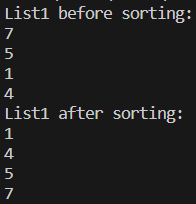
\includegraphics[width=0.25\textwidth]{Files/Billeder: Appendix/Insertion Sort Result.png}
    \end{center}
    \caption{The result for the insertion-sort code example}
    \label{figure:insetion_sort_result}
\end{figure}

\subsubsection{Code Example: Seconds Time-conversion} \label{acc_test_Seconds}

\subsubsection{Source Code in \lang:}
\begin{lstlisting}[language = scriptkid, firstnumber=1, label={list:acceptance_test_timeconversion_input}, caption=Acceptance test input of the timeconversion code example]
function mod(number a, number b) return number
{ 
    number remainder = a; 
    repeat while (remainder >= b) 
    { 
        remainder = remainder - b; 
    } 
    return remainder; 
} 
number seconds_in_minute = 60; 
number seconds_in_hour = seconds_in_minute * 60; 
number seconds_in_day = seconds_in_hour * 24; 
number seconds_in_week = seconds_in_day * 7; 
number input_seconds = call number input(); 
decimal weeks = input_seconds / seconds_in_week; 
input_seconds = call mod(input_seconds, seconds_in_week); 
decimal days = input_seconds / seconds_in_day; 
input_seconds = call mod(input_seconds, seconds_in_day); 
decimal hours = input_seconds / seconds_in_hour; 
input_seconds = call mod(input_seconds, seconds_in_hour); 
decimal minutes = input_seconds / seconds_in_minute; 
input_seconds = call mod(input_seconds, seconds_in_minute); 
call output("Number of weeks:"); 
call output(weeks); 
call output("Number of days:"); 
call output(days); 
call output("Number of hours:"); 
call output(hours);
call output("Number of minutes:"); 
call output(minutes); 
\end{lstlisting}

\subsubsection{Target Code in C:}
\begin{lstlisting}[language = c, firstnumber=106, label={list:acceptance_test_timeconversion_output}, caption=Acceptance test output of the timeconversion code example]
...
int mod(int a, int b) 
{ 
    int remainder = a; 
    while ((remainder >= b)) 
    { 
        remainder = (remainder - b); 
    } 
    return remainder; 
} 
void main() 
{ 
    int seconds_in_minute = 60; 
    int seconds_in_hour = (seconds_in_minute * 60); 
    int seconds_in_day = (seconds_in_hour * 24); 
    int seconds_in_week = (seconds_in_day * 7); 
    int input_seconds = *(int *)input("%d", sizeof(int)); 
    float weeks = (input_seconds / seconds_in_week); 
    input_seconds = mod(input_seconds, seconds_in_week); 
    float days = (input_seconds / seconds_in_day); 
    input_seconds = mod(input_seconds, seconds_in_day); 
    float hours = (input_seconds / seconds_in_hour); 
    input_seconds = mod(input_seconds, seconds_in_hour); 
    float minutes = (input_seconds / seconds_in_minute); 
    input_seconds = mod(input_seconds, seconds_in_minute); 
    printf("%s\n", "Number of weeks:"); 
    printf("%g\n", weeks); 
    printf("%s\n", "Number of days:"); 
    printf("%g\n", days); 
    printf("%s\n", "Number of hours:"); 
    printf("%g\n", hours); 
    printf("%s\n", "Number of minutes:"); 
    printf("%g\n", minutes); 
} 
\end{lstlisting}

\subsubsection{result:}

\begin{figure}[H] 
    \begin{center}
        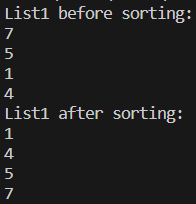
\includegraphics[width=0.25\textwidth]{Files/Billeder: Appendix/Insertion Sort Result.png}
    \end{center}
    \caption{The result for the time-conversion code example}
    \label{figure:timeconversion_result}
\end{figure}

\subsection{Code Example: GDB Calculator} \label{acc_test_Calcc}

\subsubsection{Source Code in \lang:}
\begin{lstlisting}[language = scriptkid, firstnumber=1, label={list:acceptance_test_GDB_input}, caption=Acceptance test input of the GDB calculator code example]
number divisor; 
number input_a; 
number input_b; 
number min; 
number max; 
number remainder; 
text tryAgain = "y"; 
function mod(number a, number b) return number 
{ 
    number remainder = a; 
    repeat while (remainder >= b) 
    { 
        remainder = remainder - b; 
    } 
    return remainder;   
} 
function GetMax() return number 
{ 
    if (input_a > input_b) 
    { 
        return input_a; 
    } 
    else 
    { 
        return input_b; 
    } 
    return -1; 
} 
function GetMin() return number 
{ 
    if (input_a < input_b) 
    { 
        return input_a; 
    } 
    else 
    { 
        return input_b; 
    } 
    return -1; 
} 
repeat while (tryAgain is "y") 
{ 
    comment: Asks for two positive integers as input and in the case of an error, ask the user again; 
    call output("Enter two positive integers:"); 
    boolean continue = false; 
    repeat while (continue is false) 
    { 
        input_a = call number input(); 
        input_b = call number input(); 
        if (input_a <= 0 or input_b <= 0) 
        { 
            call output("Please enter two positive integers:"); 
            continue = false; 
        } 
        else 
        { 
            continue = true; 
        } 
    } 
    max = call GetMax(); 
    min = call GetMin(); 
    continue = false; 
    number i = min; 
    repeat while(i > 0 and continue is false) 
    { 
        if (call mod(max, i) is 0 and call mod(min, i) is 0) 
        { 
            divisor = i; 
            continue = true; 
        } 
        i = i - 1; 
    } 
    call output("The biggest divisor is:"); 
    call output(divisor); 
    call output("Would you like to try again? (y/n)"); 
    tryAgain = call text input(); 
} 
\end{lstlisting}

\subsubsection{Target Code in C:}
\begin{lstlisting}[language = c, firstnumber=106, label={list:acceptance_test_timeconversion_output}, caption=Acceptance test output of the timeconversion code example]
...
int mod(int a, int b) 
{ 
    int remainder = a; 
    while((remainder >= b)) 
    { 
    remainder = (remainder - b); 
    } 
return remainder;
} 
int GetMax(int input_a, int input_b) 
{ 
    if((input_a > input_b)) 
    { 
        return input_a;
    } 
    else 
    { 
        return input_b;
    } 
    return -1;
} 
int GetMin(int input_a, int input_b) 
{ 
    if((input_a < input_b)) 
    { 
        return input_a;
    } 
    else 
    { 
        return input_b;
    } 
    return -1;
} 
void main(){ 
int divisor = 0; 
int input_a = 0; 
int input_b = 0; 
int min = 0; 
int max = 0; 
int remainder = 0; 
char * tryAgain = "y"; 
while(0 == strcmp(tryAgain, "y")) 
{ 
    printf("%s\n", "Enter two positive integers:"); 
    int continue_ = 0; 
    while((continue_ == 0)) 
    { 
    input_a = *(int *)input("%d", sizeof(int)); 
    input_b = *(int *)input("%d", sizeof(int)); 
        if(((input_a <= 0) || (input_b <= 0))) 
        { 
        printf("%s\n", "Please enter two positive integers:"); 
        continue_ = 0; 
        } 
        else 
        { 
        continue_ = 1; 
        } 
    } 
    max = GetMax(input_a, input_b); 
    min = GetMin(input_a, input_b); 
    continue_ = 0; 
    int i = min; 
    while(((i > 0) && (continue_ == 0))) 
    { 
    if(((mod(max, i) == 0) && (mod(min, i) == 0))) 
    { 
        divisor = i; 
        continue_ = 1; 
    } 
    i = (i - 1); 
    } 
    printf("%s\n", "The biggest divisor is:"); 
    printf("%d\n", divisor); 
    printf("%s\n", "Would you like to try again? (y/n)"); 
    tryAgain = (char *)input("%s", sizeof(char *));
    } 
} 
\end{lstlisting}

\subsubsection{result:}
\begin{figure}[H] 
    \begin{center}
        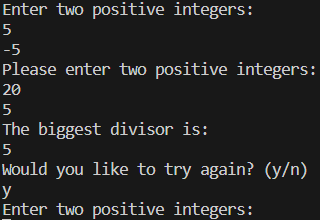
\includegraphics[width=0.40\textwidth]{Files/Billeder: Appendix/GDB Results.png}
    \end{center}
    \caption{The result for the GDB-calculator code example}
    \label{figure:repeatinput_result}
\end{figure}

\subsection{Code Example: test input \& repeat}

\subsubsection{Source Code in \lang:}
\begin{lstlisting}[language = scriptkid, firstnumber=1, label={list:acceptance_test_repeat_input_test}, caption=Acceptance test input of the repeat loops code example]
comment: Function to test repeat (x) times loop and input; 
function StartFunction() return nothing{
    text inputText; 
    boolean flag = true; 
    number repetitions; 
    repeat while(flag){ 
        call output(""); 
        call output("Write 'start' to start: "); 
        inputText = call text input(); 
        if(inputText is "start"){ 
            call output(""); 
            call output("Write amount of repetitions: "); 
            repetitions = call number input(); 
            repeat (repetitions) times{ 
                call output("This is a repeated message"); 
            }           
        } 
    } 
} 
call StartFunction(); 
\end{lstlisting}

\subsubsection{Target code in C:}
\begin{lstlisting}[language = C, firstnumber=106, label={list:acceptance_test_repeat_input_test_InC}, caption=Acceptance test input of the repeat loops code example output in C]
...
void StartFunction()
{
    char * inputText = "";
    int flag = 1;
    int repetitions = 0;
    while(flag){
        printf("%s\n", "");
        printf("%s\n", "Write 'start' to start: ");
        inputText = (char *)input("%s", sizeof(char *));
        if(0 == strcmp(inputText, "start")){
            printf("%s\n", "");
            printf("%s\n", "Write amount of repetitions: ");
            repetitions = *(int *)input("%d", sizeof(int));
            for (int number = 0; number < repetitions; number++){
               printf("%s\n", "This is a repeated message");
            }
        }
    }
}
void main(){
StartFunction();
}
\end{lstlisting}

\subsubsection{result:}
\begin{figure}[H] 
    \begin{center}
        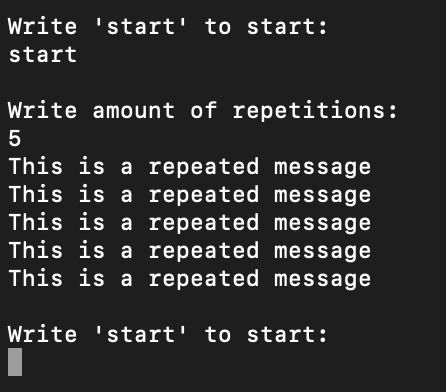
\includegraphics[width=0.40\textwidth]{Files/Billeder: Appendix/Repat And Input.png}
    \end{center}
    \caption{The result for the repeat-input code example}
    \label{figure:repeatinput_result}
\end{figure}




\subsection{Code Example: Triangle area calculate.}

\subsubsection{Source Code in \lang:}
\begin{lstlisting}[language = scriptkid, firstnumber=1, label={list:acceptance_test_triangle}, caption=Acceptance test calculating triangle code examples]
function triArea(number width, number height) return decimal
{ 
    return (width * height) / 2; 
} 
call output(call triArea(2,3)); 
call output(call triArea(7,4)); 
call output(call triArea(10,10)); 
call output(call triArea(3,3)); 
\end{lstlisting}



\subsubsection{Target code in C:}
\begin{lstlisting}[language = C, firstnumber=1, label={list:acceptance_test_triangle_output}, caption=Acceptance test triangle code examples in C]
float triArea(int width, int height)
{
    return ((width * height) / 2);
}
void main(){
printf("%g\n", triArea(2, 3));
printf("%g\n", triArea(7, 4));
printf("%g\n", triArea(10, 10));
printf("%g\n", triArea(3, 3));
}
\end{lstlisting}

\subsubsection{result:}
\begin{figure}[H] 
    \begin{center}
        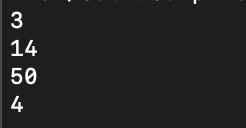
\includegraphics[width=0.40\textwidth]{Files/Billeder: Appendix/TriangleCalc.png}
    \end{center}
    \caption{The result for the calculate triangle area code example}
    \label{figure:triangleArea_result}
\end{figure}

\subsection{Mathematical Expressions} \label{test_MathExpr}

\subsubsection{Source Code in \lang:}
\begin{lstlisting}[language = scriptkid, firstnumber=1, label={list:acceptance_test_mathexpr}, caption=Acceptance test math expressions code examples]
number x = 14;
number y = 7;
number z = 10;

number A;
number B;
number C;
decimal D;
number E;

A = x + y;
B = x - y;
C = x * y;
D = x / y;
E = (x + y) * z;


call output(A);
call output(B);
call output(C);
call output(D);
call output(E);
\end{lstlisting}

\subsubsection{Target code in C:}
\begin{lstlisting}[language = C, firstnumber=1, label={list:acceptance_test_mathexpr_output}, caption=Acceptance test math expressions code examples in C]
void main(){
    int x = 14;
    int y = 7;
    int z = 10;
 
    int A = 0;
    int B = 0;
    int C = 0;
    float D = 0;
    int E = 0;
 
    A = (x + y);
    B = (x - y);
    C = (x * y);
    D = (x / y);
    E = ((x + y) * z);
 
    printf("%d\n", A);
    printf("%d\n", B);
    printf("%d\n", C);
    printf("%g\n", D);
    printf("%d\n", E);
}
\end{lstlisting}

\subsubsection{result:}
\begin{figure}[H] 
    \begin{center}
        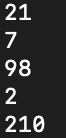
\includegraphics[width=0.10\textwidth]{Files/Billeder: Appendix/MathExpr.png}
    \end{center}
    \caption{The result for mathematical expressions code example}
    \label{figure:triangleArea_result}
\end{figure}

 number x = 5;
 text y = "this is a test"
 text z = 5;

 \subsection{Missing ";" error message} \label{test_MissingSemi}

\subsubsection{Source Code in \lang:}
\begin{lstlisting}[language = scriptkid, firstnumber=1, label={list:acceptance_test_missingsemi}, caption=Acceptance test missing ";" code examples]
 number x = 5;
 text y = "this is a test"
 text z = 5;
\end{lstlisting}

\subsubsection{result:}
\begin{figure}[H] 
    \begin{center}
        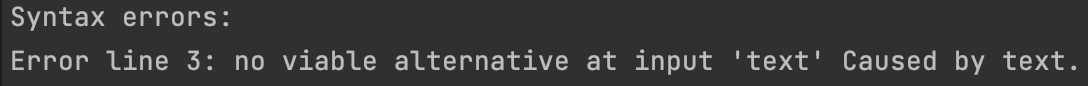
\includegraphics[width=1\textwidth]{Files/Billeder: Appendix/errormsg1.png}
    \end{center}
    \caption{The result for missing semi colon code example}
    \label{figure:errorMsg1_result}
\end{figure}


 \subsection{Wrong type error message} \label{test_TypeErr}
\subsubsection{Source Code in \lang:}
\begin{lstlisting}[language = scriptkid, firstnumber=1, label={list:acceptance_test_wrongtype}, caption=Acceptance wrong type code examples]
text y = "a";
text z = 5;
 \end{lstlisting}

 \subsubsection{result:}
\begin{figure}[H] 
    \begin{center}
        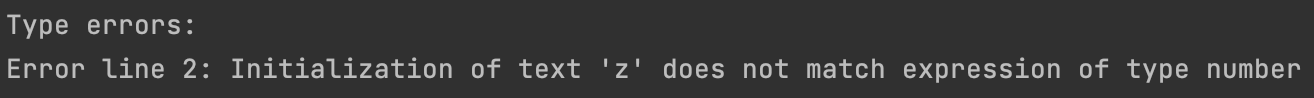
\includegraphics[width=1\textwidth]{Files/Billeder: Appendix/errormsg2.png}
    \end{center}
    \caption{The result for wrong type code example}
    \label{figure:errorMsg2_result}
\end{figure}


\subsection{String Concatenation} \label{test_stringconc}

\subsubsection{Source Code in \lang:}
\begin{lstlisting}[language = scriptkid, firstnumber=1, label={list:acceptance_test_stringconc}, caption=Acceptance test string conc code examples]
text hej = "gem" + "fem";

call output(hej);
\end{lstlisting}

\subsubsection{Target code in C:}
\begin{lstlisting}[language = C, firstnumber=1, label={list:acceptance_test_stringconc_output}, caption=Acceptance test string conc code examples in C]
char* concat(const char *str1, const char *str2) 
{
     size_t len1 = strlen(str1);
     size_t len2 = strlen(str2);
     char *result = malloc(strlen(str1) + strlen(str2) + 1);
     strcpy(result, str1);
     strcat(result, str2);
     return result;
}

void main()
{
    char * hej = concat("gem", "fem");
    printf("%s\n", hej);
}

\end{lstlisting}

 \subsubsection{result:}
\begin{figure}[H] 
    \begin{center}
        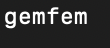
\includegraphics[width=0.2\textwidth]{Files/Billeder: Appendix/stringconc.png}
    \end{center}
    \caption{The result for string concatenation code example}
    \label{figure:stringconc_result}
\end{figure}


\subsection{Zero Division}

\subsubsection{Source Code in \lang:}
\begin{lstlisting}[language = scriptkid, firstnumber=1, label={list:acceptance_test_zerodiv}, caption=Acceptance test division by zero code examples]
number x = 5;
number y = 0;
decimal a;
decimal b;

a = x / y;
b = y / x ;


call output(a);
call output(b);
\end{lstlisting}

\subsubsection{Target code in C:}
\begin{lstlisting}[language = C, firstnumber=1, label={list:acceptance_test_zerodiv_output}, caption=Acceptance test division by zero code examples in C]
void main()
{
    int x = 5;
    int y = 0;
    float A = 0;
    float B = 0;
    
    A = (divide(x, y));
    B = (divide(y, x));
    
    printf("%g\n", A);
    printf("%g\n", B);
}
\end{lstlisting}


 \subsubsection{result:}
\begin{figure}[H] 
    \begin{center}
        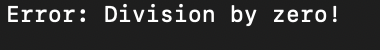
\includegraphics[width=0.4\textwidth]{Files/Billeder: Appendix/ZeroDiv.png}
    \end{center}
    \caption{The result for division by zero code example}
    \label{figure:zerodiv_result}
\end{figure}

\subsection{Symbol Table scope-fix}
\label{Appendix:ScopeFix}

\subsubsection{AddIdToFunctionBlock:}
\begin{lstlisting}[language = csharp, firstnumber=232, label={list:symbolTable_AddIdToFunction}, caption=AddIdToFunctionBlock - 134-169 - CobraCompiler/SymbolTable.cs]
public void AddIDToFunctionBlock(Symbol symbol, BlockNode blockNode)
{
    //Only add the ID if the ID is contained in a functionBlock
    //and has not already been declared within this functionBlock

    FunctionBlockNode? fBlockNode = null;

    var scope = _scopes[blockNode];

    while (scope != null)
    {
        //Has functionBlock:
        if (scope.Block is FunctionBlockNode)
        {
            fBlockNode = scope.Block as FunctionBlockNode;
        }

        //If the name is declared within the current scope, we don't add it
        if (scope.Symbols.ContainsKey(symbol.Name))
            break;

        //If has functionBlock and has not been declared yet in any scopes,
        //The ID must've been an identifier from outside the function
        if (fBlockNode != null)
        {

            if (!fBlockNode.UsedVariables.Keys.Contains(symbol.Name))
                fBlockNode.UsedVariables.Add(symbol.Name, symbol.Type);

            //Exit because we've now met a functionBlockNode
            break;
        }

        scope = scope.Parent;
    }
}
\end{lstlisting}

\subsubsection{Visit Declaration-Node:}
\begin{lstlisting}[language = csharp, firstnumber=232, label={list:symbolTable_DeclarationNode}, caption=Visit Declaration-Node - 232-250 - CobraCompiler/SymbolTable.cs]
public override ASTNode? Visit(DeclarationNode node)
{
    if (_reservedKeywords.Contains(node.Identifier.Name))
        node.Identifier.Name = $"{node.Identifier.Name}_";

    var sym = Lookup(node.Identifier.Name, _currentBlock);

    string underscores = "";
    while (sym != null)
    {
        underscores += "_";
        sym = Lookup($"{node.Identifier.Name}{underscores}", _currentBlock);
    }

    node.Identifier.Name += underscores;
    Insert(node.Identifier.Name, node.Identifier.TypeNode.Type, node);
    Visit(node.Expression);
    return null;
}
\end{lstlisting}

\subsubsection{Visit Identifier-Node:}
\begin{lstlisting}[language = csharp, firstnumber=767, label={list:symbolTable_IdentifierNode}, caption=Visit Identifier-Node - 767-792 - CobraCompiler/SymbolTable.cs]
public void Visit(IdentifierNode node)
{
    if (_reservedKeywords.Contains(node.Name))
        node.Name = $"{node.Name}_";

    var prevSym = Lookup(node.Name, _currentBlock);
    var currSym = Lookup($"{node.Name}_", _currentBlock);

    string underscores = "_";
    while (currSym != null)
    {
        prevSym = currSym;
        currSym = Lookup($"{node.Name}{underscores}", _currentBlock);
        underscores += "_";
    }

    node.Name = prevSym.Name;

    if (prevSym != null)
        AddIDToFunctionBlock(prevSym, _currentBlock);

    if (prevSym == null)
    {
        SymbolError(node, $"{node.Name} is not found. Declare your variable before use.");
    }
}
\end{lstlisting}
\end{document}